%%%%%%%%%%%%%%%%%%%%%%%%%%%%%%%%%%%%%%%%%
% Short Sectioned Assignment
% LaTeX Template
% Version 1.0 (5/5/12)
%
% This template has been downloaded from:
% http://www.LaTeXTemplates.com
%
% Original author:
% Frits Wenneker (http://www.howtotex.com)
%
% License:
% CC BY-NC-SA 3.0 (http://creativecommons.org/licenses/by-nc-sa/3.0/)
%
%%%%%%%%%%%%%%%%%%%%%%%%%%%%%%%%%%%%%%%%%

%----------------------------------------------------------------------------------------
%	PACKAGES AND OTHER DOCUMENT CONFIGURATIONS
%----------------------------------------------------------------------------------------

\documentclass[paper=a4, fontsize=18pt]{article} % A4 paper and 11pt font size
\usepackage{lmodern}
\usepackage[T1]{fontenc} % Use 8-bit encoding that has 256 glyphs
\usepackage{graphicx}
\usepackage{subfigure}
%\usepackage{fourier} % Use the Adobe Utopia font for the document - comment this line to return to the LaTeX default
\usepackage[english]{babel} % English language/hyphenation
\usepackage{amsmath,amsfonts,amsthm} % Math packages
\usepackage[linesnumbered,ruled,vlined]{algorithm2e}
\usepackage{lipsum} % Used for inserting dummy 'Lorem ipsum' text into the template
\usepackage{sectsty} % Allows customizing section commands
\usepackage{hyperref}
%\allsectionsfont{\centering \normalfont\scshape} % Make all sections centered, the default font and small caps

\usepackage{fancyhdr} % Custom headers and footers
\usepackage{multirow}
%\usepackage{multicolumn}
\pagestyle{fancyplain} % Makes all pages in the document conform to the custom headers and footers
\fancyhead{} % No page header - if you want one, create it in the same way as the footers below
\fancyfoot[L]{} % Empty left footer
\fancyfoot[C]{} % Empty center footer
\fancyfoot[R]{\thepage} % Page numbering for right footer
\renewcommand{\headrulewidth}{0pt} % Remove header underlines
\renewcommand{\footrulewidth}{0pt} % Remove footer underlines
\setlength{\headheight}{13.6pt} % Customize the height of the header
\setlength{\parskip}{0.5\baselineskip}

\numberwithin{equation}{section} % Number equations within sections (i.e. 1.1, 1.2, 2.1, 2.2 instead of 1, 2, 3, 4)
\numberwithin{figure}{section} % Number figures within sections (i.e. 1.1, 1.2, 2.1, 2.2 instead of 1, 2, 3, 4)
\numberwithin{table}{section} % Number tables within sections (i.e. 1.1, 1.2, 2.1, 2.2 instead of 1, 2, 3, 4)

\newcommand{\mM}{\mathcal{M}}
\newcommand{\mL}{\mathcal{L}}
\newcommand{\mB}{\mathcal{B}}
\newcommand{\mT}{\mathcal{T}}
\newcommand{\mS}{\mathcal{S}}
\newcommand{\mP}{\mathcal{P}}
\newcommand{\bH}{\mathbb{H}}

\setlength\parindent{0pt} % Removes all indentation from paragraphs - comment this line for an assignment with lots of text

\graphicspath{{pic/}}

%----------------------------------------------------------------------------------------
%	TITLE SECTION
%----------------------------------------------------------------------------------------
\newtheorem{definition}{Definition}{\itshape}{\rmfamily}
\newtheorem{theorem}{Theorem}{\itshape}{\rmfamily}
\newtheorem{corollary}{Corollary}{\itshape}{\rmfamily}
\newtheorem{example}{Example}{\itshape}{\rmfamily}
\newtheorem{proposition}{Proposition}{\itshape}{\rmfamily}
\newcommand{\horrule}[1]{\rule{\linewidth}{#1}} % Create horizontal rule command with 1 argument of height

\title{	
\normalfont \normalsize
\horrule{0.5pt} \\[0.4cm] % Thin top horizontal rule
\huge Survey for Spatial and Temporal Data Bases and Mining \\ % The assignment title
\horrule{2pt} \\[0.5cm] % Thick bottom horizontal rule
}
\hypersetup{hidelinks}

\author{Naiqi Li \hspace*{0.5cm} Jianzhong Qi \hspace*{0.5cm} Rui Zhang\\
\vspace{-.1cm}\\
\emph{Department of Computing and Information Systems}\\
\emph{The University of Melbourne}\\
\small naiqil@student.unimelb.edu.au \{jianzhong.qi, rui.zhang\}@unimelb.edu.au}


\date{} % Today's date or a custom date

\begin{document}

\maketitle % Print the title
\tableofcontents





\section{Contextual Intent Tracking for Personal Assistants \cite{SYWXMZ16}}

This paper focuses the new paradigm of recommendation that recommends ``the right information at the right time'', which requires tracking users' contemporaneous intent. It proposes the Kalman filter regularized PARAFAC2 (KP2) nowcasting model, which compactly represents the structure and co-movement of context and intent. This paper shares many core ideas with a previous study \cite{SYXMZ16}.

The paper models each contextual signal as a random process which produces a time series. The contextual signals include activities that user engage in such as the apps being used, venues users visit, real-time spatial measurements, etc. All the contextual signals for a user $u$ form a panel, which is denoted by $X^u$.

\begin{figure}[h]
  \centering
  % Requires \usepackage{graphicx}
  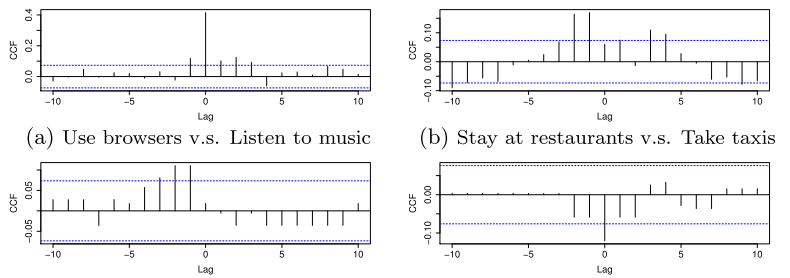
\includegraphics[width=.8\linewidth]{8_22_ccf2.png}\\
  \caption{Sequential correlation between contextual signals and intent}\label{fig:ccf2}
\end{figure}

It is shown that there is sequential correlation between context and intent by using the cross-correlation coefficient (CCF). CCF measures the similarity of two series at different lags. Figure \ref{fig:ccf2} shows the CCF at various lags between some contextual signal and intent. For example from Figure \ref{fig:ccf2} (a) we can see that while using browsers (content), users often intend to listen to music (intent), because the two series have a significantly large CCF at zero.
There is also correlation between contextual signals, which is shown by the covariance between different contextual signals.

The basic idea of the proposed KP2 model is to represent the structure and dynamics of panels with low-dimensional latent factors, and utilize the evolution of these latent factors for intent tracking.

\begin{figure}[h]
  \centering
  % Requires \usepackage{graphicx}
  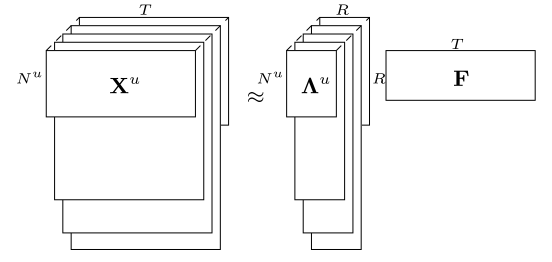
\includegraphics[width=.5\linewidth]{8_22_ccf.png}\\
  \caption{PRAFAC2 decomposition}\label{fig:ccf1}
\end{figure}

To obtain a compact model, the interactions among contextual signals and intent are represented by a few low-dimensional latent factors:
$$X^u \approx \Lambda^u F^u,$$
where $X^u \in \mathbb{R}^{N^u \times T}$ is the panel of user $u$, $F^u \in \mathbb{R}^{R \times T}$ contains the latent factors, and $\Lambda^u \in \mathbb{R}^{N^u \times R}$ is called the factor loading matrix. It further proposes to utilize the collaborative capabilities among all the users. Specifically, the latent factors $F^u$ are represented by shared factors $F$. So the model becomes
$$X^u \approx \Lambda^u F.$$
Such latent factors can be obtained with the PRAFAC2 tensor decomposition by organizing all panels into a tensor and aligning them by the time dimensions. Figure \ref{fig:ccf1} illustrates the formed tensor and PARAFAC2 decomposition.

To enforce sequential correlation, and enable efficient and robust-to-noise intent computation, the paper proposes using Kalman filter to regularize the latent factors, and uses the obtained dynamic system for real-time intent nowcasting. Kalman filter introduces a transition system matrix $A^u$, and noise covariance matrices $\Psi^u$ and $Q^u$. Latent factors obtained with Kalman filter not only compactly represent the panel structure shared by all users, but also model the common temporal dynamics and sequential correlation within all panels.

After obtaining the latent factors $F$, transition matrix $A^u$, loading matrix $\Lambda^u$, and noise covariance matrices $\Psi^u$ and $Q^u$, the method builds a personalized dynamic system for each user. Specifically, it first estimates priori latent factors $\tilde{f}_t$ for the current time step $t$. When contextual signals $x_t^u$ are continuously available, it computes posteriori latent factors $\tilde{f}$ with Kalman filter, and then uses the regression technique for intent nowcasting.

The proposed method involves solving the optimization problems. The paper presents the gradient computation of the parameters, and then uses stochastic gradient descent (SGD) to find the optimized parameter values.

In the experimental section, the method is evaluated on dataset from a commercial personal assistant. The performance is evaluated based on the F-measure and Hit-ratio, where the F-measure evaluates the precision and recall of model predicted intent, and hit-ratio measures the model's user coverage. When compared with other approaches, it is shown that the proposed model us up to 3.5 times better in F-measure, and the hit-ratio is consistently the best across all predicted intents.


\section{{INSQ:} An influential neighbor set based moving kNN query processing system \cite{Li0QYZD16}}

This article is based on a previous paper \cite{Li0QYZ014}, which proposes an algorithm called the \emph{Influential Neighbor Set (INS)} to process the \emph{moving $k$ nearest neighbor (M$k$NN)} query.

Given a query point $q$, a M$k$NN query computes its $k$ nearest neighbor set and maintains it while $q$ is moving. Recall that INS uses a small set of safe guarding objects instead of safe regions. As long as the current $k$ nearest neighbors are closer to the query object than the safe guarding objects, the current $k$ nearest neighbors stay valid and no recomputation is required.

The new contribution of this paper is that it showcases a system called \emph{INSQ}, which is based on the INS algorithm. The presented system is able to process the M$k$NN queries in both two-dimensional Euclidean space and road networks.

The system is implemented as a Scala Swing application. The application runs in two modes, \emph{Road Network} mode and \emph{2D Plane} (Euclidean space) mode. Its user interface consists of two panels (cf. Figure \ref{fig:INSQ1}):

1) Control panel. This is the left panel of the user interface. It is used for setting the demonstration parameters, which include the Global Setting, the Road Network setting and the 2D Plane setting.

2) Main panel. It displays a map of a road network where data objects (orange dots) and the query object (red dot) can be placed onto. Users can specify a trajectory for the query object. In the Road Network mode, this trajectory must confine the underlying road network; in the 2D Plane mode, the trajectory can have any shape. When query simulation starts, the query object will move along the specified trajectory. The INS algorithm will run to compute the $k$NN set and the INS set, which are shown as the green dots and the yellow dots respectively.


\begin{figure}[h]
  \centering
  % Requires \usepackage{graphicx}
  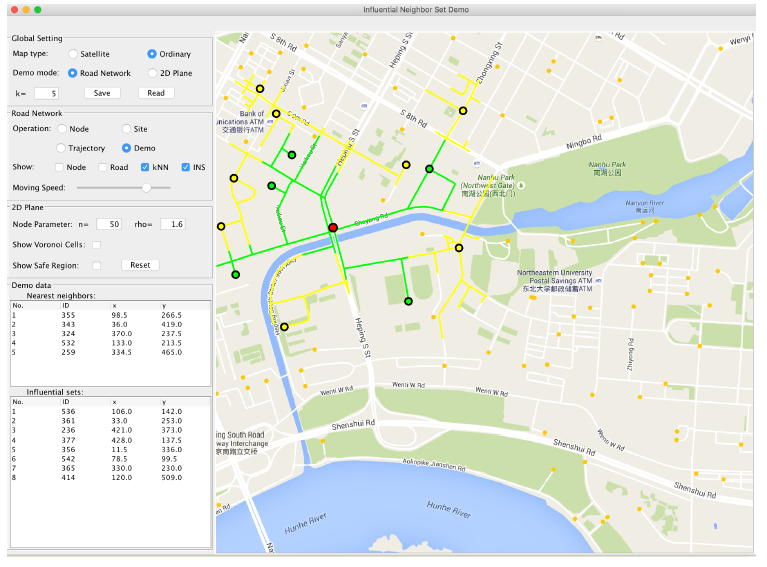
\includegraphics[width=.7\linewidth]{9_12_kNN1.png}\\
  \caption{Screenshot of Road Network mode}\label{fig:INSQ1}
\end{figure}
\begin{figure}[h]
  \centering
  % Requires \usepackage{graphicx}
  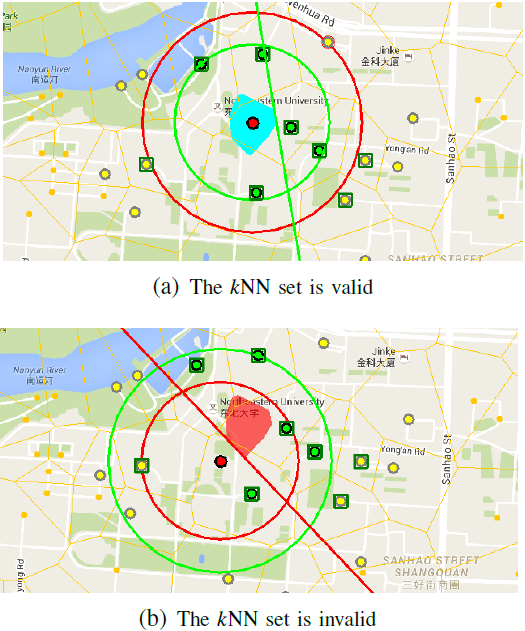
\includegraphics[width=.4\linewidth]{9_12_kNN2.png}\\
  \caption{Screenshots of 2D Plane mode}\label{fig:INSQ2}
\end{figure}

The paper takes the 2D Plane mode as an example. Figure \ref{fig:INSQ2} displays two screenshots of the demonstration program, where each shows: 1) the query object stays in the order-$k$ Voronoi cell of the current $k$NN set; 2) the query object has moved out of the order-$k$ Voronoi cell. When the query object moves out of the order-$k$ Voronoi cell shown in Figure \ref{fig:INSQ2} (a) and moves into the position shown in Figure \ref{fig:INSQ2} (b), the current $k$NN set becomes invalid since the green circle is now enclosed by the red circle (i.e., the farthest object to $q$ in the $k$NN set is farther to $q$ than the nearest object to $q$ in the INS).



\section{Reverse Nearest Neighbor Heat Maps: A Tool for Influence Exploration \cite{SZXQD16}}

This paper studies the problem of constructing a \emph{reverse nearest neighbor (RNN)} heat map by finding the RNN set of every point in a two-dimensional space. It proposes an algorithm called \emph{CREST (Constructing RNN hEat map with the Sweep line sTrategy)} that efficiently solves the \emph{Region Coloring (RC)} problem. It also performs detailed analyses on the complexity of CREST and prove that CREST is asymptotically optimal.

\begin{figure}[h]
  \centering
  % Requires \usepackage{graphicx}
  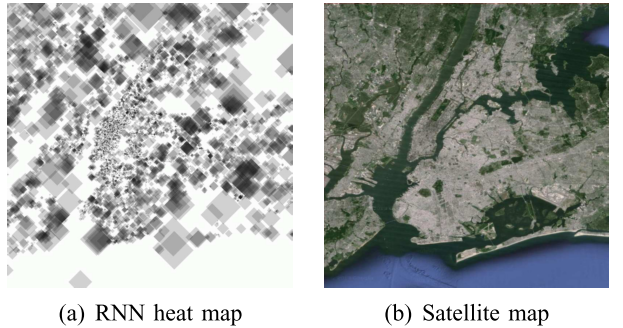
\includegraphics[width=.6\linewidth]{8_22_rnnheat.png}\\
  \caption{RNN heat map of New York City}\label{fig:heat}
\end{figure}

The RNN heat map shows the influence of every point in the space, where the influence of the location is commonly measured by the set of its RNNs. Figure \ref{fig:heat} shows such an RNN heat map for the New York City. It enables exploring the influence of the whole space while considering qualitative factors.

Instead of computing the influence value of every point in the space, the problem can be reduced to the RC problem, which divides the space into disjoint regions, within which all the points have the same RNN set. For each point $o$, it draws a ``circle'' called the \emph{NN-circle} with $o$ being the center, and the distance to $o$'s nearest neighbor (NN) being the radius. (The following discussion uses the $L_\infty$ distance so the NN-circles are rectangles.) The NN-circles partition the space into separate regions. It is proved that all the points in such a region have the same RNN set, so also have the same heat. The RC problem is to obtain the influence of each such region in the space.

\begin{figure}[h]
  \centering
  % Requires \usepackage{graphicx}
  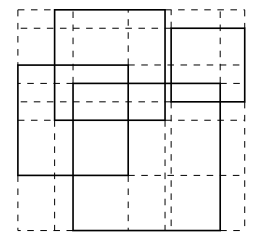
\includegraphics[width=.3\linewidth]{8_22_side.png}\\
  \caption{Side extension}\label{fig:side}
\end{figure}

A simple approach to the RC problem is to pick a point $p$ inside each region, and obtain the NN-circle that enclose $p$ and then label the region. Another naive method is to extend the sides of each NN-circle to let them span across the whole space and form a grid (cf. Figure \ref{fig:side}). Then it scans the grid cells and computes the RNN set for the centroid of each cell. However, all these methods have two main drawbacks: 1) they need to process point enclosure queries; 2) a region in the original partition will be labeled multiple times. Next we will see how the CREST algorithm overcomes these two drawbacks.

\begin{figure}[h]
  \centering
  % Requires \usepackage{graphicx}
  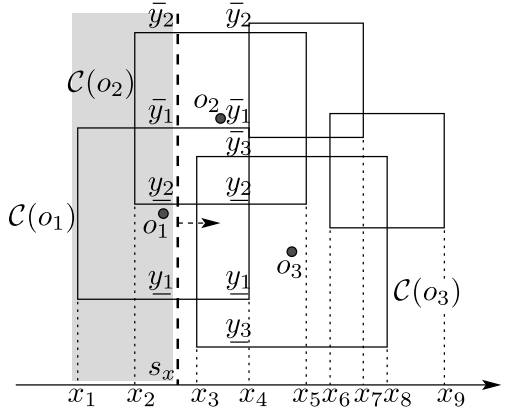
\includegraphics[width=.5\linewidth]{8_22_sweep.png}\\
  \caption{Example of the sweep line strategy}\label{fig:sweep}
\end{figure}

The CREST algorithm employs the classic \emph{sweep line strategy} to avoid forming a large number of cells to be labeled. It lets a line sweep from the left to the right of the space, and stores information about the NN-circles that are currently cut by the sweep line. As illustrated in Figure \ref{fig:sweep}, it uses the distinct vertical sides as event points (i.e., $x_1, x_2, ..., x_9$). When the line sweeps to the right, some of the subregions come from the same original region, and hence do not require the repetitive RNN set and influence computations. In this way, it avoids to lable a region multiple times.

The second proposed technique aims to avoid the RNN computation with point enclosure queries. The basic idea is to utilize the fact that the RNN set of a region can be obtained efficiently by modifying the RNN set of the adjacent regions.

The paper also discusses how to apply the CREST algorithm in different settings: 1) CREST directly applies to the monochromatic RNNs; 2) in two-dimensional spaces, the $L_1$ distance can be viewed as equivalent to the $L_\infty$ distance by rotation and scaling; 3) CREST still applies to $L_2$ distance metric but requires modification, since a partition is formed by curved edges.

In the experimental section, the paper evaluates the proposed method in terms of CPU time. It is shown that CREST outperforms alternative algorithms by up to three orders of magnitude.

\section{MOOCs Meet Measurement Theory: A Topic-Modelling Approach \cite{HRBZMC16}}

This paper combines a machine learning technique (topic modelling) with measurement theory (psychometrics) as used in education. It introduces a novel regularisation into \emph{non-negative matrix factorisation}-based topic modelling, so the discovered topics conform to a \emph{Guttman scale}.

\begin{figure}[h]
  \centering
  % Requires \usepackage{graphicx}
  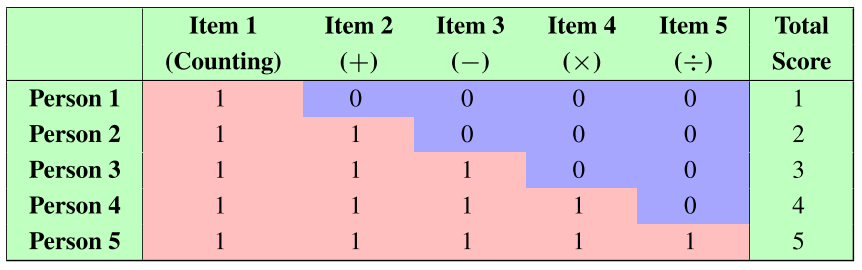
\includegraphics[width=.8\linewidth]{8_22_Guttman.png}\\
  \caption{An example of a perfect Guttman scale measuring mathematical ability}\label{fig:Guttman}
\end{figure}


\emph{Measurement} in education and psychology is the process of assigning a number to an attribute of an individual in such a way that individuals can be compared to another. A Guttman scale induces a total ordering on items, so that an individual who successfully answers a particular item also answers items of lower rank-order. For example Figure \ref{fig:Guttman} shows a perfect Guttman scale measuring mathematical ability. Intuitively, if a student can calculate Division, she is also able to solve the other simpler problems.

The goal of this paper is to automatically generate items (topics) from unstructured forum data using topic modelling, such that the discovered topics conform to a Guttman scale. For example, for a MOOC on discrete optimisation, the goal is to automatically discover topics such as \emph{How to us platform/python} (the easiest problem), and \emph{How to design and tune simulated annealing and local search} (a more difficult topic).

\emph{The paper chooses Non-Negative Matrix Factorisation (NMF)} as the basic approach to discover topics due to the interpretability of the produced topics. Given a non-negative matrix $V \in \mathbb{R}^{m \times n}$ and a positive integer $k$, NMF factorises $V$ into the product of two non-negative matrices $W \in \mathbb{R}^{m \times k}$ and $H \in \mathbb{R}^{k \times n}$: $V \approx WH$. Thus, NMF involves solving the following optimisation problem:
$$\min_{W,H} \| V - WH \|_F^2 \mbox{ s.t. } W \geq 0, H \geq 0.$$

Recall that the goal of this paper is to generate a set of meaningful topics that yield a matrix conforming to the properties of a Guttaman scale, e.g., a near-triangular matrix. In other words, it requires that the topic-student matrix $H$ be binary, and Guttman-scaled. Next we will see how to add regularization terms to achieve these two goals.

The new proposed objective function is:
$$f(W,H) = \| V - WH \|_F^2 + \lambda_0 \| W \|_F^2 + \lambda_1 \| H - H_{ideal} \|_F^2 + \lambda_2 \| H \circ H - H \|_F^2.$$
\begin{itemize}
\item $\| W \|_F^2$ prevents overfitting;
\item $\| H - H_{ideal} \|_F^2$ encourages a Guttman-scaled $H$, where $H_{ideal}$ is a constant matrix with ideal Guttman scale;
\item $\| H \circ H - H \|_F^2$ encourages $H$ to be a binary ($\circ$ denotes element-wise product). It is equal to $\| H \circ (H - 1) \|_F^2$, which is clearly minimised by binary $H$.
\end{itemize}
Finally a local optimum is achieved via iteration rules derived from the \emph{Karush-Kuhn-Tucker conditions}.

In the experimental section, the paper adopts the \emph{Coefficient of Reproducibility (CR)}, which measures how well a student's responses can be predicted given his/her position on the scale. It is shown that the proposed method maintains good quality of approximation (only up to 8\% worse than the standard NMF since there are more constraints). As for the ROC and precision-recall curves, the proposed method significantly dominates NMF with around 20\%-30\% better performance. The paper also provides qualitative survey on the interpretability of the generated topics.

\section{Scalable Hypergraph Processing \cite{HZY15}}

This paper studies large scale \emph{hypergraph} processing in a distributed environment. It proposes \emph{HyperX}, which is a thin layer built upon Spark, for easily implementing hypergraph learning algorithms.

\begin{figure}[h]
  \centering
  % Requires \usepackage{graphicx}
  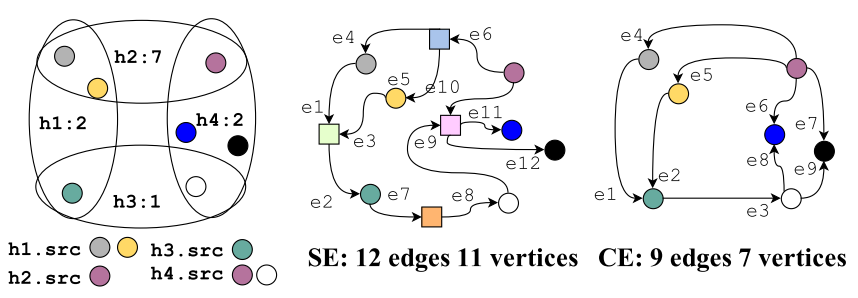
\includegraphics[width=.6\linewidth]{8_15_HyperX1.png}\\
  \caption{Converting a hypergraph to a graph}\label{fig:HyperX1}
\end{figure}

A hypergraph differs from a graph in that it allows hyperedges to connect more than two vertices, using which to capture the high-order relationships. For example in Figure \ref{fig:HyperX1}, the hyperedge $h1$ connects both the grey and yellow nodes to the green node. When learning larger hypergraphs, a common approach is converting them to graphs to employ the distributed graph framwork. The \emph{Star-Expansion (SE)} method treats each hyperedge as a new vertex, and the \emph{Clique-Expansion (CE)} treats each hyperedge as a clique among the related vertices. Figure \ref{fig:HyperX1} demonstrates an example of converting a hypergraph following these two approaches.

After the conversion, existing methods apply the distributed graph framework for hypergraph learning. The hypergraph is divided into partitions, and each partition is distributed to and processed by a computing node. However, such approach has several major drawbacks: 1) The conversion can result in a prohibitively large graph; 2) An enormous replication cost. Each vertex may be replicated to many different nodes for local processing; 3) A great difficulty in balancing workloads. Next we will see how the HyperX method can avoid all these shortcomings.

\begin{figure}[h]
  \centering
  % Requires \usepackage{graphicx}
  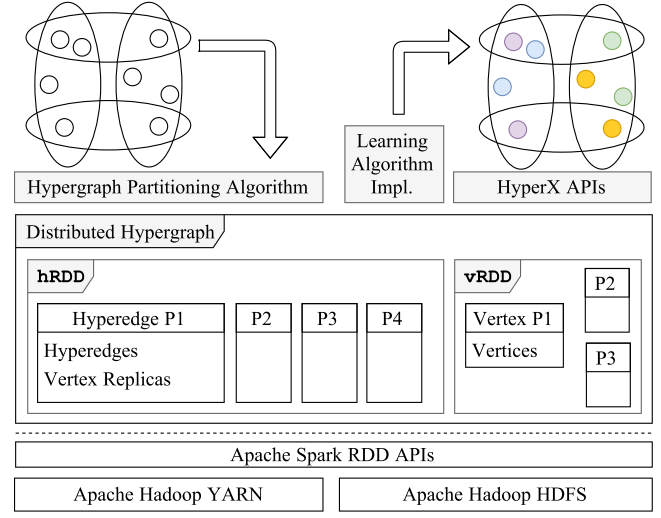
\includegraphics[width=.7\linewidth]{8_15_HyperX2.png}\\
  \caption{An overview of HyperX}\label{fig:HyperX2}
\end{figure}

An overview of HyperX is represented in Figure \ref{fig:HyperX2}. Without converting a hypergraph, HyperX directly stores a hypergraph as two RDDs, vRDD for the vertices and hRDD for the hyperedges (\emph{Resilient Distributed dataset (RDD)} is a read-only multiset of data items distributed over a cluster of machines in a fault-tolerant way). Each vertex and each hyperedge is stored as one row. The vRDD simply stores the id and value of a vertex. The hRDD flattens each hyperedge to multiple tuples.

Next we will see how HyperX supports hypergraph learning algorithm, and how does it achieve workload balancing.

Hypergraph learning algorithms usually involve accessing and updating the weights of relations and the value of vertices. HyperX provides two program interfaces: \emph{vProg} that updates the value of a vertex according to its related hyperedges, and \emph{hProg} that updates the weight of each hyperedge according to the related vertices.

Workload balancing is a very important factor for the performance. HyperX distributes the workloads by partitioning vertices and hyperedges and assigning them to the distributed workers. The paper uses a \emph{hybrid-cut} approach which partitions both vertices and the hyperedges. The goal of applying the hybrid-cut technique is to minimize  the communication cost between different workers. The communication cost is mainly due to when vProg is working, the related hyperedge values must be sent over the network from distributed workers.

The paper describes how three common hypergraph learning algorithms can be implemented easily using HyperX, which are \emph{random walks}, \emph{label propagation}, and \emph{spectral learning}.

The experimental section studies the memory consumption of data RDDs, the network communication cost, and the elapsed time of the three learning algorithms. It is reported that when compared with the most competitive previous work, the proposed method consumes 48\% to 77\% less memory, communicates 19\% to 98\% less data, and the elapsed time is reduced by up to 49.1 times.

\section{HEADS-JOIN: Efficient Earth Mover's Distance Similarity Joins on Hadoop \cite{HZBCW16}}

This paper is an extension of a previous work \cite{HZBC14}, which proposes a \emph{MapReduce (MR)} based framework for \emph{Earth Mover's Distance (EMD)} similarity range joins. The main extra contribution of this paper is that it extends the previous framework by designing algorithms for the \emph{Bulk Synchronous Parallel (BSP)} and the \emph{Spark} paradigms. The extended framework is name \emph{Hadoop EArth mover's Distance Similarity Join (HEADS-JOIN)}.

Recall that the similarity join retrieves all the pairs of objects such that the similarity between the two objects is higher than a threshold. In this paper, the EMD metric defines the dissimilarity as the minimal transformation cost between two data objects.

The basic idea of HEADS-JOIN is the same as that of the previous work. The computation follows the following three main steps (which was presented in a previous document with more details):
1) Transform data objects into spaces corresponding to multiple \emph{normal lower bounds} of EMD.
2) Divide the transformed spaces using a set of grids based on the lower bounds, and group the transformed records into composite cells.
3) Compute the lower bound of the EMD between every record and every cell. Any $\langle record, cell \rangle$ pair that has a lower bound of EMD greater than the threshold is pruned. The remaining $\langle record, cell \rangle$ pairs will go through further refinement step.

Next I will present the new extensions of this paper, that is, how to solve this problem with BSP and Spark paradigms.

The BSP paradigm is a generic computation paradigm designed for parallel computation units. In BSP, computations are executed on parallel workers in the fashion of consecutive \emph{supersteps}. In each superstep, each worker first computes independently using the local data, then sends messages to each other, and reads messages sent to them in a synchronous barrier.

The BSP approach has two phases, i.e., the preparation phase and the  pruning and refining phase. The preparation phase works as follows. Each worker reads a portion of the data and applies the normal-LB transformation. Then each worker sends the transformed data to one master worker, who uses the second superstep to aggregate the domain and the quantile values. After the master workers are finished, they send these values to all the workers. Each worker uses the third superstep to prepare information such as the aggregation errors in each local cell (which are used to compute the lower bounds). Again, master workers will receive these results and compute the global aggregated result. In the last superstep, all the workers use the feedback information to partition data. The second phases conducts the actual pruning and the refining.

Apache Spark is the open source implementation of \emph{Resilient Distributed Dataset (RDD)}, and is fully compatible to the Hadoop platform.

The Spark approach also has two phase: one for preparing the grids, and one for filtering and refining. The goal of the preparing phase is to: 1) construct the grid structures; 2) aggregate the error and bound values for each cell; 3) assign cells to workers based on the workload estimation. Similarly, the second phase conducts the actual pruning and produces the final results.

In the experimental section, the new results include a comparison of the three paradigms (MR, BSP, and Spark) with the \emph{Quickjoin} method \cite{JS08}. It is reported that the speedup factors are up to 3, 6.1, and 4.0 in range joins respectively. The best choice among the three paradigms depends on the dataset, and there is not a consistent winner.

\section{MARS: Mobile Application Relaunching Speed-up through Flash-Aware Page Swapping \cite{GCFWZZ16}}

This paper presents the design, implementation, and evaluation of \emph{MARS}, a retrofitted Linux page swapping for fast application relaunching on smartphones.

Since users usually run the same application multiple times and use several applications simultaneously, improving the performance of application relaunching is very important. In current mobile platforms, applications are cached in memory. However, this causes two main drawbacks: 1) the memory size is limit and only moderate numbers of applications can be cached; 2) as applications become much more complex, it is difficult to restore to the previous states. This paper tries to use the page swapping technique to mitigate these two issues.

However, the page swapping technique is not directly applicable to current Android systems. The most critical reason that Android has disabled page swapping in Linux kernel is the incompatibility between page swapping and Android \emph{runtime garbage collection (runtime GC)}: If the page swapping technique is naively implemented, since the garbage objects are usually not touched until runtime GC is started, those objects should be more likely to be swapped. When runtime GC finally runs, lots of garbage objects need to be swapped out and then the system only discovers that they are indeed garbage and should be discarded.

To address these compatibility and performance issues, MARS aims to replace Linux page swapping on Android in order to improve the performance of application relaunching.

The first step is to resolve the conflicts between page swapping and Android runtime GC by isolating them. MARS achieves this by modifying both Linux swapping and Android runtime framework. For example runtime GC is frozen until the application comes back to the foreground, so runtime GC will never conflict page swapping

There are two components in MARS to further improve the performance: \emph{page slot allocation}, and \emph{read/write control}.

Page slot allocation aims to reduce scattered reads. This is motivated by the observation \emph{that eMMC (Embedded Multi Media Card)} on smartphones has poor scattered I/O performance. It is indicated that the scattered read operation is up to ten times slower than the sequential read operation. MARS proposes a method to organize pages of an application in a sequential \emph{LBA (Logic Block Address)} sequence in swap area and make them swap in together.

Read/write control aims to reduce the interference of flash reads and writes. This is motivated by the fact that concurrent reads and writes interfere with each other in flash memory based Solid State Drivers (SSD) and cause performance degradation severely. MARS proposes a method to decouple swap-out and swap-in by using a novel swapping control mechanism.

In the experimental section, the paper evaluates the performance of MARS against the original Linux page swapping and the current solution on Android. Micro-benchmarks have verified that both components of MARS achieve the initial design goals. Evaluation results also show that MARS reduces the launching time of Android applications by 50\% to 80\%.

\section{Exploiting velocity distribution skew to speed up moving object indexing \cite{NH0W15}}

This article is an extended version of a previous paper \cite{NHZW12}, which proposes the \emph{velocity partitioning (VP)} technique that exploits the skew in velocity distribution to speed up query processing of moving objects.

The system proposed in the previous paper has two main components, a \emph{velocity analyzer} and an \emph{index manager}. The velocity analyzer partitions the velocities of objects in order to find the \emph{dominant velocity axes (DVAs)}. This technique is a combination of \emph{principal components analysis (PCA)} and \emph{$k$-means} clustering. The index manager maintains an index tree for each DVA. When an object needs to be inserted, the index manager first finds the DVA index $i_{min}$ whose perpendicular distance from the object is the smallest. Then the manage inserts the object to the index $i_{min}$. Here the underlying index structure ($i_{min}$) can be a TPR-tree, a B$^x$-tree or their variants. Other operations like deletion and update are also similarly performed.

This paper extends the previous work in three aspects. First, it presents an algorithm for the \emph{$k$-nearest neighbor ($k$-NN) query} based on the VP technique. Second, it proposes the \emph{RCG (RAM-resident compressed grid)} index which improves the performance of the outlier index by exploiting the characteristics of SSDs. Third, it extends the experimental evaluation to include $k$-NN queries and the impact of the RCG index.

The first technique is to use the index manager to handle $k$-NN queries. Given a moving point $q_p$, and a query time $t_q$, a $k$-NN query retrieves a set of $k$ nearest objects from $q_p$ at time $t_q$. The basic idea is to iteratively perform range queries with an incrementally increasing search region on each of the indexes separately, until the exact $k$-nearest objects are found. Similar to the algorithm for range queries, it first needs to transform the query point to the coordinate system of the DVA index. After querying all indexes, if the number of objects in the result set is less than $k$, the index manager increases the search region and repeats the process. Otherwise, the manager returns the current $k$ nearest objects to $q_p$ as the query results.

\begin{figure}[h]
  \centering
  % Requires \usepackage{graphicx}
  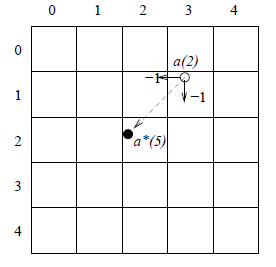
\includegraphics[width=.4\linewidth]{9_12_VP1.png}\\
  \caption{Example of inserting an outlier}\label{fig:VP1}
\end{figure}

The second technique is to improve the performance of the outlier index by making use of SSDs, which is motivated by the fact that the outlier index occupies a disproportionately high percentage of the CPU time (up to 60\%). This SSD friendly version of the outlier index is called RCG (RAM-resident compressed grid). The basic idea is to reduce CPU time by completely caching outliers in a RAM-resident grid structure, since the grid structure has been found to yield better query performance for indexes reside in RAM. Specifically, each cell of the grid stores compressed object information indexed based on object location. In order to handle the time dimension, it takes the same approach as the B$^x$-tree, namely, expanding the query by the maximum velocity within the grid. For example in Figure \ref{fig:VP1}, an object $a$ at update time 2 is inserted into a time bucket with reference time 5. First, $a$ is converted to the reference time 5 shown as $a^*$. Then $a^*$ is inserted into the grid cell which contains the object at time unit 5.

\begin{figure}[h]
  \centering
  % Requires \usepackage{graphicx}
  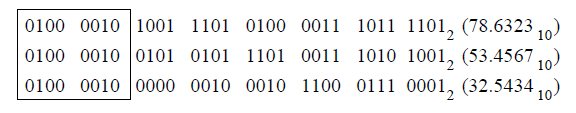
\includegraphics[width=.7\linewidth]{9_12_VP2.png}\\
  \caption{Example of applying location compression on the x-location column}\label{fig:VP2}
\end{figure}

In order to maintain the RCG index in main memory, the paper further proposes methods to compress the information of outlier objects within each grid cell. The simple approach is achieved by storing the objects' information column-by-column. For example, Figure \ref{fig:VP2} shows the relative values of x-location column and their binary representation (relative locations are smaller in magnitude and can be compressed more). Next, it finds the longest sequence which is the same for all values, and stores these values once for all the objects. The paper also investigates a lossy compression method to further reduce the size of the index.

In the experimental study, the new results show that when the VP technique is combined with the B$^x$-tree, for the $k$NN queries the performance is improved by up to 3 and 2 times in terms I/O cost and CPU time, respectively. It is also shown that the RCG  index consistently outperforms the disk-based index.

\section{Destination Prediction by Identifying and Clustering Prominent Features from Public Trajectory Datasets \cite{YXLZ15}}

This paper proposes a discriminative method, called \emph{PROminent Feature Identification and cLustEring (PROFILE)}, for solving the destination prediction problem.

 \begin{figure}[h]
  \centering
  % Requires \usepackage{graphicx}
  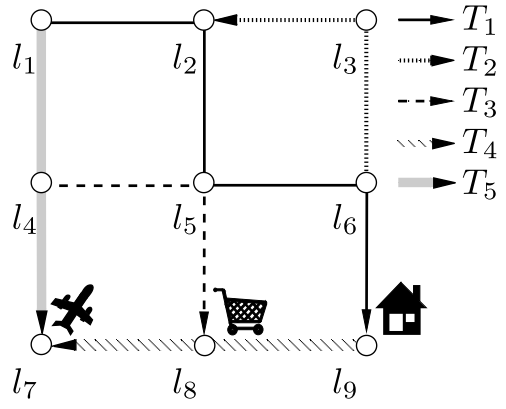
\includegraphics[width=.6\linewidth]{7_25_dest_pred.png}\\
  \caption{An example of destination prediction}\label{fig:dest}
\end{figure}

The problem of destination prediction was discussed in a previous paper summary of \cite{XZZXHX13}.
Figure \ref{fig:dest} presents an example destination prediction problem. There are five historical trajectories $T_1, ..., T_5$, and each of them is represented by a different type of line. Suppose that now a client is moving from $l_1$ to $l_4$, and this query trajectory partially matches $T_5$. Therefore, the destination of $T_5$ (i.e. $l_7$) is the predicted destination of the query trajectory.

The PROFILE technique works as follows. It first decomposes each trajectory to several partial segments. For example, $\{n_1, n_4, n_5\}$ will be decomposed into three partially-finished trajectories $\{n_1\}, \{n_1, n_4\}$ and $\{n_1, n_4, n_5\}$. These partial trajectories are used as the training dataset, and the most prominent features such as current location and the travel direction are extracted. Then the partial trajectories are grouped into different clusters based on the features. Within each cluster, the algorithm computes a predicted destination by averaging the destinations for all partial trajectories. When a query trajectory is given, it finds the cluster it belongs to, and returns the pre-computed predicted destination of that cluster.

In this paper four representative features are used. The following two features are used as the directional information: 1) the direction from the starting location to the current location; 2) the direction of the last two locations. These two directional features are categorised into North, East, South, and West. The other two features are the current location, and the travel distance.

The clustering step is achieved by hashing, where partial trajectories with the same features will be put into the same cluster. In other words, all partial trajectories in a single cluster have the same four features.
Then the predicted destination for each cluster is defined as:
$$(\hat{x}, \hat{y}) = \arg \min_{(\hat{x}, \hat{y})} \frac{1}{k} \sum_{i=1}^k | \hat{x} - x_i | + | \hat{y} - y_i|.$$
Here $k$ is the number of trajectories in a cluster.

In the experimental section, the paper shows that PROFILE is better than a previous approach in terms of both runtime efficiency and prediction accuracy. In the best cases, the improvement is about two orders of magnitude in running time, and the distance deviation decreases about 3km.

\section{K-Nearest Neighbor Temporal Aggregate Queries \cite{SQZ015}}

This paper proposes a new type of queries called the $k$-nearest neighbor temporal aggregate ($k$NNTA) query, which can retrieve points of interest (POIs) by integrating the spatial distance and a temporal aggregate on a certain attribute. It designs a novel index called the TAR-tree to support the efficient processing of the $k$NNTA query. It also performs a detailed analysis on the cost of the proposed data structure.

Given a query point and a time interval, a $k$NNTA query returns the top-$k$ locations that have the smallest weighted sums of the spatial distance from the query point, and a temporal aggregate on a certain attribute over the time interval. For example, find a nearby club that has the largest number of check-ins in the last hour.

The proposed TAR-tree is a variant of the R-tree, and the algorithms for indexing the spatial extents of the POIs remain the same. The key difference between the TAR-tree and R-tree is that each entry of the TAR-tree also points to a temporal index. The temporal index stores the aggregate over each epoch, and keeps each record as a triple $\langle t_s, t_e, agg \rangle$, where $t_s$ is the start time and $t_e$ is the end time of the epoch, and $agg$ is the aggregate value. The temporal index is called temporal index on the aggregate (TIA).

\begin{figure}[h]
  \centering
  % Requires \usepackage{graphicx}
  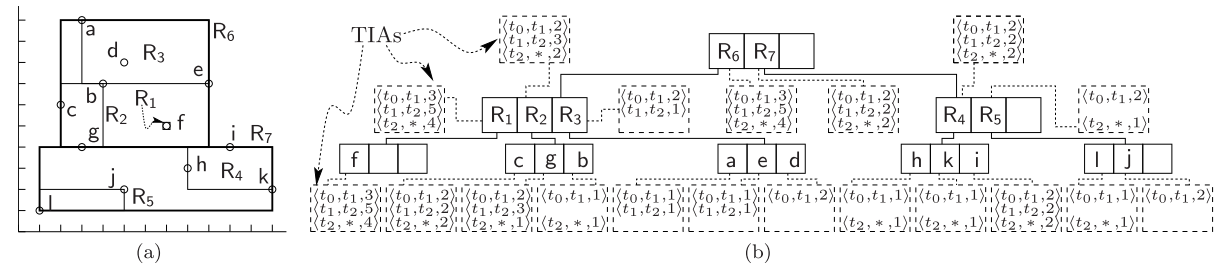
\includegraphics[width=.9\linewidth]{8_15_TAR.png}\\
  \caption{TAR-tree example}\label{fig:TAR}
\end{figure}

Figure \ref{fig:TAR} presents an example of TAR-tree indexing the POIs. Figure \ref{fig:TAR} (a) shows the MBRs of the entries, and Figure \ref{fig:TAR} (b) shows the index structure.

The insertion and deletion of TAR-tree are similar to the counterparts of R-tree, but the group strategy is different when several entries are to be indexed by the same node. A good grouping strategy is also the most important aspect for a TAR-tree to work efficiently.

The paper introduces two naive strategies for grouping the entries. The first approach is to group the entries entirely based on the spatial extents, which means that the TAR-tree behaves the same as the R-tree. Another straightforward strategy is to group the entries that have similar aggregate distributions. The similarity or distance between two distributions can be measured by the Manhattan distance. When a POI is added, it is inserted into the node that has the smallest distance to it. Then the paper proposes a more sophisticated grouping strategy, called the integral 3d strategy. The method groups the entries by integrating the spatial and aggregated information to minimize the node extents. Specifically, it groups the entries as 3-dimensional bounding boxes, in which two are the spatial dimensions and the third is a dimension capturing the aggregate information.

In the experimental section, the paper measures the performance of the TAR-tree in terms of CPU time and the number of node access. It is shown that the TAR-tree outperforms a baseline algorithm by up to two orders of magnitude in CPU time, and 3 times in the number of node access.

\section{Skyline Trips of Multiple POIs Categories \cite{AHZ15}}

This paper proposes a new path finding problem, called \emph{Skyline Trips of Multiple POIs Categories (STMPC)}, which finds the skyline trips of multiple \emph{Point of Interest (POI)} categories between two points based on cost and distance. It presents two heuristic algorithms to compute the approximate solution for the proposed problem.

Given a road network graph $G$, source $s$ and destination $d$, a set of categories $C = \{c_1,...,c_n\}$ with a set $P$ of POIs in each category $c_i = \{p_1, ..., p_n\}$, the STMPC query involves two optimality dimensions, which are the cost aggregated from POIs, and the distance cost. The query returns a set of trips that are not dominated in terms of both trip length and trip aggregated cost.

\begin{figure}[h]
  \centering
  % Requires \usepackage{graphicx}
  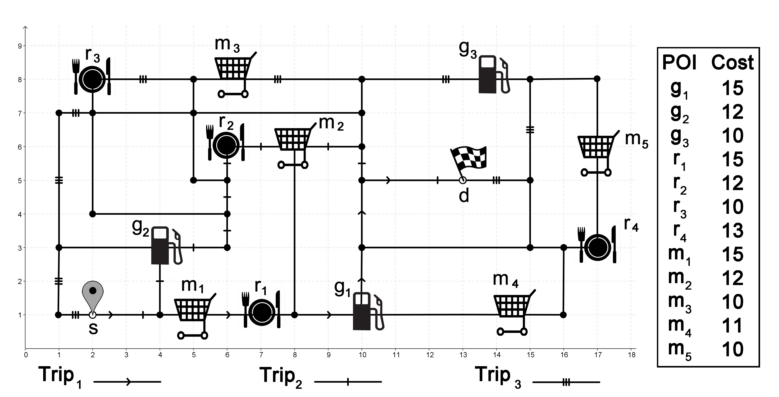
\includegraphics[width=.6\linewidth]{8_15_skyline.png}\\
  \caption{Example of STMPC query}\label{fig:STMPC}
\end{figure}


For example in Figure \ref{fig:STMPC} a user at $s$ wants to visit one POI from each category (gas station, restaurant, and supermarket) on his way to $d$. For instance, $Trip_1 = \{s,m_1,r_1,g_1,d\}$ has the distance (15) with aggregated cost (45). Any other trip has higher trip length or aggregated cost, so $Trip_1$ is one of the skyline query result.

The paper shows that the STMPC query is a generalization of the well known\emph{\emph{ Travelling Salesman Problem (TSP)}}. The basic idea is that if the aggregated cost is 0 for each POI, and each node is associated with a different category, then the only skyline trip is also the shortest path that visits every node. Consequently the STMPC query is NP-hard. Since the proposed problem is theoretically difficult, the paper tries to solve it by providing approximated results.

The first method is called the \emph{Weighted POIs (WPOIs)} algorithm. The WPOIs algorithm is divided into two stages: POIs nomination stage and trip construction stage, and it works by repeatedly iterating through these two stages. In the POI nomination stage, each POI is associated with two properties, the estimated distance $p^d$ (which is heuristically defined as the aggregated Euclidean distance from both $s$ and $d$), and the POI cost $p^c$. The priority value is $p^p = w^c p^c + w^d p^d$, where $w^c$ and $w^d$ are dependent weights that $w^c + w^d = 1$. The algorithm gradually adjusts the weights in each iteration. For the given weights, each POI category nominates a POI with the least priority value. In the trip construction stage, the algorithm needs to find a path that goes through each nominated POI. Since this can be viewed as TSP, the paper uses the same technique used to solve the TSP problem in the trip construction stage.

The second proposed method is called the \emph{Clustered Weighted POIs (CWPOIs)} algorithm. One problem with the previous WPOIs algorithm is that, the estimated distance only considers the length between a POI and the source and destination. However, the distance between one POI and another is also important. The CWPOIs algorithm addresses this problem by clustering POIs in geographical regions (POIs in the same Quadtree nodes) in advance. Next it performs a skyline query over the Quadtree nodes by the first algorithm (WPOIs), where the outcome is a set of nominated nodes. The remaining steps are constructing skyline trips and producing the result, which are the same as WPOIs.

In the experimental study, the paper evaluates the effectiveness and efficiency of the proposed algorithms. It is reported that both algorithms return skyline trips that are close to optimal trips (about 0.9-0.98 in optimaplity metric) within reasonable running time (less than 10s). The algorithms are four orders of magnitude faster than a naive solution.

\section{Identifying At-Risk Students in Massive Open Online Courses \cite{HBRZ15}}

The paper proposes a method to early identify students who are at risk of not completing courses in \emph{Massive Open Online Courses (MOOCs)}. Based on \emph{Logistic Regression (LR)}, it proposes two transfer learning algorithms to trade-off smoothness and accuracy.

MOOCs such as Coursera and edX are facing a major problem: low completion rates. The goal of this paper is to make early prediction that can help instructors design interventions to encourage course completion before a student falls too far. To make the prediction useful and meaningful, it should be accurate, well-calibrated and smoothed across week.

The basic idea is based on logistic regression. The paper proposes two transfer learning algorithm to trade-off smoothness and accuracy by adding a regularization term to minimize the difference between consecutive weeks.

The first proposed algorithm is called \emph{Sequentially Smoothed LR (LR-SEQ)}, which uses the previous week's knowledge to help learn smoothed probabilities for the current week. Let $x_i^{(i-1,i)}$ denote the set of students in week $i$ that also exist in week $i-1$, and similarly let $x_{i-1}^{(i-1,i)}$ denote the set of students in week $i-1$ that also exist in week $i$. The objective function is defined to be:
$$\mL(w_i) = \sum_{j=1}^{n_1} \log(1+\exp(-y_j w_i^T x_{ij})) + \frac{\lambda}{2} \| w_i \|^2 + \lambda_2 \sum_{j=1}^{n_{i,i-1}} \|w_i^T x_{ij}^{(i,i-1)} - w_{i-1}^T x_{i-1j}^{(i,i-1)}\|^2.$$
The first part of the formula is the standard logistic regression. The second part is the regularization term for avoiding overfitting. The third part is proposed in this paper, where parameter $\lambda_2$ controls the smoothness level.

The second proposed algorithm is called \emph{Simultaneously Smoothed LR (LR-SIM)}. The drawback of the first approach LR-SEQ is that week $i$'s model is built based on the model of week $i-1$, so early inaccurate predictions cannot benefit from the knowledge learned in later weeks. The first step is to extend the feature space for each student $x_{ij}$ to a new space with $n$ components (where $n$ is the current week). For example the student $j$ at the end of week 2, $x_{2j}$ is extended to $x_{2j}'$ in the matrix:
\begin{center}
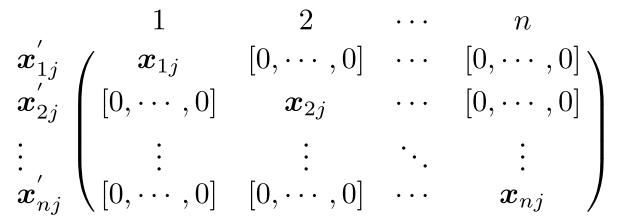
\includegraphics[width=.6\linewidth]{8_15_MOOC.png}
\end{center}
Based on the extended $x_{ij}'$, the algorithm can minimize the difference of probabilities predicted for different weeks together, via the objective function:
$$\mL(w) = \sum_{i=1}^n \sum_{j=1}^{n_1} \log(1+\exp(-y_j w_i^T x_{ij})) + \frac{\lambda}{2} \|w_i\|^2 + \lambda_2 \sum_{i=2}^n \sum_{j=1}^{n_{i,i-1}} \|w_i^T x_{ij}^{(i,i-1)} - w_{i-1}^T x_{i-1j}^{(i,i-1)}\|^2.$$
The most significant difference between the two algorithms is that LR-SIM allows early and later predictions to be correlated and to influence each other.

In the experiment section, the paper compares the proposed algorithms with two baselines, LR and a simple method using moving averages, denoted as LR-MOV. It is reported that LR-SIM and LR-SEQ outperform the other algorithms consistently in terms of smoothness, with LR-SIM outperforming LR-SEQ.

\section{The Safest Path via Safe Zones \cite{AQJZHW15}}

This paper formulates a new problem called the \emph{Safest Path via Safe Zones (SPSZ)}, which is to find a path that minimizes the distance traveled outside a set of discrete safe zones. It proposes algorithms to process the query in both \emph{Euclidean} and \emph{spatial network} settings.

The basic idea of the method is to transform the data space with safe zones into a discrete graph, on which shortest path algorithms like Dijkstra's algorithm are applied. A naive approach is to transform each safe zone into a vertex, and add an edge between every pair of vertices with a weight that equals the unsafe distance between them. However, this yields $N(N-1)/2$ edges (where $N$ is the number of safe zones), and is very inefficient because most edges will never be used in any safest path.

\begin{figure}[h]
  \centering
  % Requires \usepackage{graphicx}
  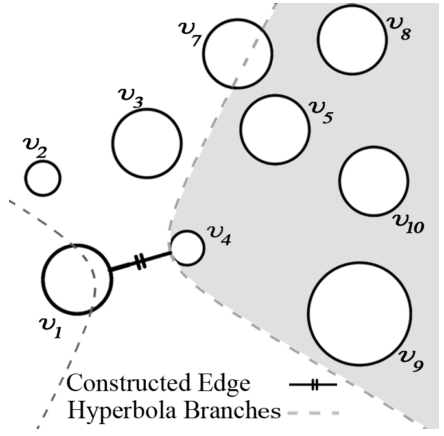
\includegraphics[width=.5\linewidth]{8_15_SPSZ.png}\\
  \caption{Pruning with hyperbola in Euclidean space}\label{fig:SPSZ}
\end{figure}

In the Euclidean space, it is observed that the regions containing the vertices with superfluous edges can be elegantly described by \emph{hyperbolas}, and the paper proposes an algorithm to utilize this property to prune unpromising edges. Figure \ref{fig:SPSZ} illustrates the main idea. Assume that we are constructing edges between $v_1$ and the other vertices in the graph. First, we construct an edge between $v_1$ and its nearest vertex $v_4$. Then we use the hyperbola branch closer to $v_4$ to divide the data space into two parts. The paper proves that to reach any point in the shaded part from $v_1$, the shortest path must go through $v_4$. So many edges can be omitted during the construction, such as edges $v_1v_5$ and $v_1v_8$.

When solving the SPSZ problem in the spatial network setting, the previous approach is not directly applicable because the hyperbola definition does not apply to network distance. But the idea still can be adapted. The paper proposes the concept of network hyperbola, which is a set $H$ of points in a spatial network, where each point $p \in H$ satisfies
$$|dist_R(f_1, p) - dist_R(f_2, p)| = k,$$
where $f_1, f_2$ are the foci of the network hyperbola, and $k$ is a constant. With the help of the network hyperbola, the paper proposes an algorithm to solve the SPSZ problem in the spatial network, which is very similar to its counterpart in the Euclidean space.

In the experimental section, the paper compares the proposed method with two naive solutions. It is reported that the number of edges created by the proposed method is an order of magnitude smaller than that of the other approaches, which validates its pruning power. It is also shown that the time taken for edge creation and query processing is smaller up to an order of magnitude.

\section{MapReduce Based Location Selection Algorithm for Utility Maximization with Capacity Constraints \cite{SQZCD15}}

This paper proposes a \emph{MapReduce} based algorithm to solve the problem of \emph{Location Selection for Utility Maximization (LSUM)}. To fully exploit the capability of parallelism, it proposes an arc-based search space partitioning strategy and a dynamic load balancing strategy.

LSUM was discussed in a previous document as well, where a centralized algorithm was presented. There is a set of \emph{clients} $C$ and a set of \emph{facilities} $F$. Each client is served by her nearest facility and each facility $f$ is constrained by a \emph{service capacity} $v(f)$. The goal of the query is to find all the locations on which if a new facility with a given capacity is established, the number of served clients is maximized.

\begin{figure}[h]
  \centering
  % Requires \usepackage{graphicx}
  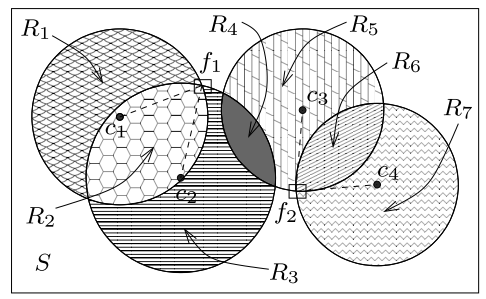
\includegraphics[width=.5\linewidth]{8_15_LSUM1.png}\\
  \caption{Some concepts}\label{fig:LSUM1}
\end{figure}

Let $f$ be a facility, we use the \emph{influence set} of $f$, denoted as $b(f)$, to represent all clients that are served by $f$. For example in Figure \ref{fig:LSUM1}, $b(f_1) = \{c_1, c_2\}, b(f_2) = \{c_3, c_4\}$. We use $u(f)$ to denote the \emph{utility} of a facility $f$, which is decided by its clients in $b(f)$ and its capacity. When adding a new facility at $f_n$, the total utility will change from $u(F)$ to $u(F \cup \{f_n\})$. The goal of LSUM can be defined as finding a $f_n$ that can maximize the increase in total utility.

In the previous paper \cite{SHCZD12}, an algorithm is proposed based on the concept of \emph{Nearest Facility Circle (NFC)} and \emph{maximal region}. The NFC of a client $c$, denoted as $n(c)$, is a circle that centers at $c$ with a radius as the distance between $c$ and its closest facility. For example $R_1 \cup R_2$ is the NFC of $c_1$ in Figure \ref{fig:LSUM1}. The NFCs divides each other into maximal regions, such as $R_1, ..., R_7$ in Figure \ref{fig:LSUM1}. It is proved that all points in the maximal region have the same influence set. So to find the optimal locations, the algorithm need too search each of the maximal regions.

\begin{figure}[h]
  \centering
  % Requires \usepackage{graphicx}
  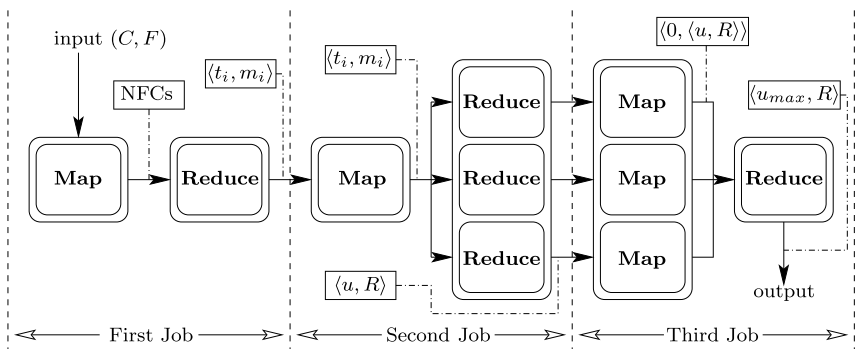
\includegraphics[width=1\linewidth]{8_15_LSUM2.png}\\
  \caption{Algorithm overviwe}\label{fig:LSUM2}
\end{figure}

In this paper, the MapReduce technique focuses on the maximal region generation process. The basic idea is to divide the data space into partitions and search the maximal regions in each partition synchronously. Finally the local results are merged to the final result. The whole process is achieved by three MapReduce jobs (cf. Figure \ref{fig:LSUM2}): 1) Search space partitioning; 2) Local optimal region searching; 3) Result merging.

In the search space partitioning job, the algorithm divides the search space based on the NFCs. The output is partitions in the form of key-value pair $\langle t_i, m_i \rangle$, where $t_i$ is the partition ID and $m_i$ denotes the data of the partition (facilities, clients, influence sets and NFCs). This job is performed on a single machine.

The input of the second job is partitions to be searched and the outputs are in the form of $\langle u, R \rangle$, where $u$ is the utility value, and $R$ is the region that achieves the utility. The map phase simply distributes the partitions based on their IDs to the reducers. In reduce phase, the reducers search for local optimal regions in parallel.

In the last job, the algorithm just need to identify the global optimal regions from the local optimal results.

The paper also proposes the search space partitioning and load balancing techniques to further improve the efficiency. To avoid the overlaps between partitions, the paper proposes to use the arcs from the NFCs to divide the space, so each maximal region is assigned to a single partition. As for load balancing issue, the paper uses a dynamic assignment strategy. In each iteration, it computes the average workload per partition, and subdivide the partitions whose workloads are larger than the average by a threshold.

In the experimental section, the paper studies the effect of different parameters on the performance, and compares the proposed algorithm with a centralized method. The results show that the proposed MapReduce based algorithm outperforms the alternative significantly (with improvement up to 30\% in response time). The effectiveness of the partitioning and workload strategies is also validated by the experimental results.


\section{A Safe Region based Approach to Moving KNN Queries in Obstructed Space \cite{Li0QZY15}} \label{sec:obs}

This paper studies the problem of processing the \emph{Obstructed Moving $k$ Nearest Neighbor (OM$k$NN) query}, i.e., the $k$NN query for a moving query point in a space with obstacles. It proposes a safe region based algorithm to efficiently process the query.

The basic idea is inspired by \emph{V$^*$-Diagram} \cite{NZTK08}, which is the state-of-the-art method for the \emph{M$k$NN query} in a space without obstacles. V$^*$-Diagram is a \emph{safe region} based technique. Specifically its safe region is computed by the following steps: 1) Let $q_b$ denote the current position of query point, and $z$ denote the $(k+x)^{th}$ nearest data point. Compute the \emph{known region}, which is a circular region centered at $q_b$ with the radius $d(q_b, z)$ ($d(x,y)$ is the distance between $x$ and $y$); 2) Compute the \emph{safe region w.r.t. a data point} $p$. Intuitively, this is a region that when the query point $q$ moves within, $p$ is nearer to $q$ than any point outside the known region; 3) Compute the \emph{fixed-rank region} where the order of distances of the $k+x$ data points to $q$ does not change; 4) Finally compute the intersection of the safe regions of the $k+x$ data points and the fixed-rank region, and the result is called the \emph{Integrated Safe Region (ISR)}. As long as $q$ remains in the ISR, its $k$NNs will not change.

\begin{figure}[h]
  \centering
  % Requires \usepackage{graphicx}
  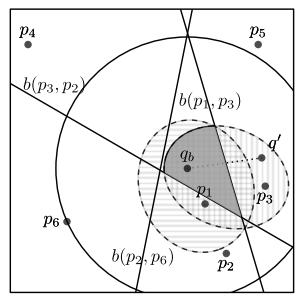
\includegraphics[width=.5\linewidth]{8_8_oisr1.png}\\
  \caption{Integrated safe region}\label{fig:oisr1}
\end{figure}

For example as Figure \ref{fig:oisr1} demonstrates, when $k = 2$ and $x = 2$ the ISR is computed to be the grey region. It is the intersection of the two safe regions w.r.t. data points $p_1$ and $p_2$ (which are the two ellipses), and the fixed rank region (which is formed by the three bisectors $b(p_1,p_3), b(p_2, p_6)$ and $b(p_3, p_2)$).

However, with the present of obstacles in the space things are becoming much more complex. All the three important concepts mentioned above (known region, safe region w.r.t. data points, and fixed-rank region) need to be adapted.

\begin{figure}[h]
  \centering
  % Requires \usepackage{graphicx}
  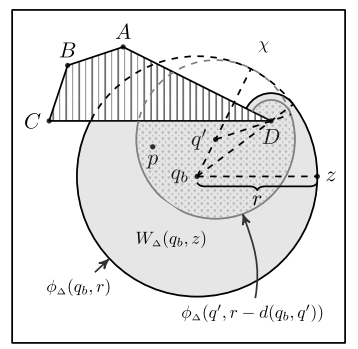
\includegraphics[width=.5\linewidth]{8_8_oisr2.png}\\
  \caption{Example of obstructed known region}\label{fig:oisr2}
\end{figure}

The \emph{obstructed known region} is no longer a circular region. For example, the grey region in Figure \ref{fig:oisr2} is the new known region with the obstacle $ABCD$. In this paper, the basic idea to compute the obstructed known region is to take into account the vertices of the obstacle. Intuitively as we see in Figure \ref{fig:oisr2}, the region is formed by several circles centered at $q$ or vertices of the obstacles.

Similarly, the \emph{Obstructed Safe Region w.r.t a Data Point (OSRD)} is no longer an ellipse. In this paper, OSRD is computed through making use of obstacle vertices, and the \emph{visible ellipse part (VEP)}. Given the query point $q_b$ and data point $p$, VEP of $q_b$ and $p$ is the part of their standard safe region that is visible from both of them. It is proved that OSRD consists of several VEPs, and based on the result an algorithm is proposed to combine VEPs to OSRD.

\begin{figure}[h]
  \centering
  % Requires \usepackage{graphicx}
  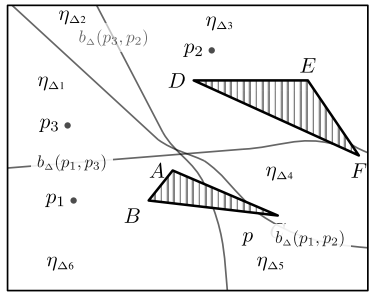
\includegraphics[width=.5\linewidth]{8_8_oisr3.png}\\
  \caption{Example of OFR}\label{fig:oisr3}
\end{figure}

The \emph{obstructed fixed-rank region (OFR)} is also different. Without the obstacles a fixed-ranked region is form by several bisectors that are straight lines, but now the bisectors could be curves (Figure \ref{fig:oisr3}). Therefore instead of computing and storing the OFR, the proposed method checks if the distance order is unchange with the \emph{Dominating Relationship Check (DRC)} algorithm.

Finally, OSRD and OFR are combined to form the \emph{Obstructed Integrated Safe Region (OISR)}, such that as long as the query point $q$ moves within OISR its $k$NNs will not change.

The paper also discusses how to choose the $x$ extra data points, which can be viewed as a cache to reduce the frequency of safe region recomputation. The paper introduce a concept called the \emph{essential auxiliary set (EAS)} to constrain the search of the $x$ extra data points. It is proved that any data point not in EAS will have no effect on the OISR result. So after obtaining the EAS, it only need to sort the result and choose the $x$ nearest data points.

The experimental section measures the performance of the proposed method in terms of the number of page accesses, the communication and the average response time, and makes comparison with a baseline algorithm. It is reported that the proposed method outperforms the baseline algorithm by up to two orders of magnitude under various settings.

\section{Solving the Data Sparsity Problem in Destination Prediction \cite{XQX0HL15}}

This article is an extended version of a previous paper \cite{XZZXHX13}. The study aims to derive the probability of a location being the destination based on historical trajectories.

Recalled that the main difficulty in destination prediction is the ``data sparsity problem'', i.e., the available historical trajectories are far from being able to cover all possible trajectories. The basic idea of \emph{SubSyn} is to use the \emph{Bayesian inference framework}, and uses a \emph{first order Markov model} to efficiently compute the posterior probability for any trajectory. Specifically, the previous paper first defines the concept of \emph{total transition probability} $p_{i \rightarrow k}$ as:
$$p_{i \rightarrow k} = (M^{l_{ik}}\sum_{r=0}^{l_{de,ik}} M^r)_{ik}.$$
Here $M$ is the transition matrix, $l_{ik}$ is the $l_1$ distance between nodes $n_i$ and $n_k$, $l_{de,ik}$ is the \emph{detour distance} from $n_i$ to $n_k$ defined as $l_{de, ik} =\lceil \alpha l_{ik} \rceil$ where $\alpha$ is the \emph{detour factor}. The intuition is to sum up all the probabilities of paths with length from $l_{ik}$ to $\lceil \alpha l_{ik} \rceil$. It does not consider any path with length greater than $\lceil \alpha l_{ik} \rceil$, because it corresponds to a path much longer than the shortest path and therefore is quite usual.

The new contributions of this paper are as follows. First, it proposes an improved training algorithm called \emph{SubSynE} (E for efficiency) that reduces the training time by more than five orders of magnitude. Second, it improves the prediction accuracy by up to 20\% by integrating the \emph{second-order Markov model}. The resultant method is called \emph{SubSynEA} (A for accuracy). Third, it proposes two additional grid partitioning strategies that result in more even number of points in each cell.

The motivation of SubSynE is that when computing $p_{i \rightarrow k}$, neither factor is sparse  even though $M$ itself is. Therefore time complexity of $O(m^3)$ is still high since it cannot apply sparse matrix multiplication techniques to reduce the time complexity. The new technique is based on the observation that, in the transition matrix $M$ there are at most four non-zero entries in each row, i.e., a user can only travel directly from one cell to its four adjacent cells. As a result, multiplying two $m \times m$ transition matrices only requires $4m^2$ multiplications. With this technique, the new algorithm is able to run on much finer grid and to further improve prediction accuracy.

The substantially improved runtime efficiency enables the paper to investigate more computationally expensive techniques such as higher-order Markov models and finer grid partition, which are presented as follows.

A naive way to apply the second-order Markov model is to use three-dimensional matrix for the transition matrix $M$, because in the second-order Markov model the transition is defined to be amongst three states: the current state and two previous state. The paper proposes a method to confine the transition matrix to remain in two-dimensional space. The basic idea is to represent transition probability as that of travelling from an edge $e_i$ to an adjacent edge $e_j$.

The paper discovers that the detour factor $\alpha$ becomes less important as the grid is more refined and dataset becomes larger. The reason is that the unusual behaviour of detour mostly comes from the process of grid partitioning rather than actual detour taken by drivers, and a larger dataset reduces the effect of $\alpha$ because a larger dataset contains more samples, which makes the model more deterministic and less random. Thus, this paper sets $\alpha$ to zero. This change further simplifies the algorithm and reduces the space usage and the running time.

The previous paper assumes using a uniform grid to represent the map, while this paper investigates other partitioning strategies: a quantile-based grid partitioning and a $k$-d tree based grid partitioning. It is demonstrated mathematically that these strategies yield more balanced number of points in each cell, achieve smaller information loss than a uniform grid, and lead to better prediction accuracy. In the quantile-based strategy, the map is represented with a grid, but the grid cells have different size following the quatile distribution of the trajectory data points. In the $k$-d tree based partition strategy, since each non-leaf node divides the data points into two half-space, it divides the the space using either horizontal or vertical lines into two partitions of equal number of points. This process is repeated until a desired grid granularity is reached.

In the experimental study, the new results show that the training of SubSynEA requires only a few minutes to run for a fine granularity of grid partitioning, while the previous SubSyn algorithm needs more than 17 hours to train a Markov model on a medium granularity grid. SubSynEA can also predict destinations for up to ten times more query trajectories than a baseline prediction algorithm.

\section{Analysis and evaluation of the top-k most influential location selection query \cite{CHWHTZ15}}

This article is an extended version of a previous paper \cite{HWQZCH11}. The study proposes a new type of queries to retrieve the \emph{top-$k$ most influential locations} from a candidate location set $C$, given a set of customers $M$ and a set of existing facilities $F$.

Recall that the previous paper proposes two branch-and bound algorithms for the query, namely \emph{Estimate Expanding Pruning (EEP)} and \emph{Bounding Influence Pruning (BIP)}.  The two algorithms exploit various geometric properties to prune the search space, and both of them use R-trees and R-tree variants to index the datasets. Their details are presented in a previous summary of \cite{HWQZCH11}.

The new contribution of this paper is that it further proposes a \emph{Nearest Facility Circle Join (NFCJ)} algorithm. With analysis of detailed steps, it shows that NFCJ achieves best $O(n \log n)$ and worst $O(n^2)$ time complexity, beating all other known algorithms for the query. It also conducts a comprehensive experimental study to compare all algorithms in terms of both CPU time and I/O performance.

Similar to the sequential scan, NFCJ involves two steps: 1) computing influence relationship between the existing facilities and customers (a facility influences a customer if it is the nearest existing facility to the customer); 2) computing influence values (how many customers are influenced if the candidate location is chosen) for candidates. The difference between NFCJ and the sequential scan is that NFCJ leverages spatial indexes to enhance the efficiency of both steps.

\begin{figure}[h]
  \centering
  % Requires \usepackage{graphicx}
  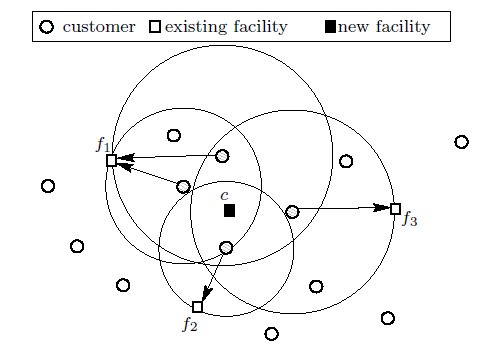
\includegraphics[width=.5\linewidth]{9_5_TopK.png}\\
  \caption{$c$ lies in 4 nearest facility circles so its influence value is 4}\label{fig:TopK}
\end{figure}

In the first step, the algorithm needs to compute the \emph{nearest facility circle} for each customer location. The nearest facility circle of a customer $m$ is a circle centered at $m$, with a radius as the distance between $m$ and its nearest facility. A new facility would be the nearest one of a customer $m$ if and only if it located in the nearest facility circle of $m$. That is to say, the potential influence of a candidate location can be computed as the number of the circles the candidate lies in. For example in Figure \ref{fig:TopK}, the new facility $c$ is located in four nearest facility circles, therefore its potential influence is 4. To help determine which circles a candidate location lies in, the algorithm constructs an R-tree on the nearest facility circles.

When computing the influence value of each candidate, the candidates are considered individually, which does not benefit from batch processing. The paper further proposes to construct another R-tree on the candidate set, such that the influence computation step can be done via an intersection join between this candidate R-tree and influence R-tree computed in the first step. Specifically, this is achieved by replacing the point enclosure query by an intersection join procedure over the two R-trees.

It the cost analysis, it is shown that both EEP and BIP are of complexity $O(n \log n)$ in the best case, and with $O(n^4)$ and $O(n^3)$ complexities respectively in the worst case. NFCJ achieves $O(n \log n)$ in the best case and $O(n^2)$ in the worst case.

In the experimental study, the new results show that NFCJ is the most efficient algorithm in terms of both time and the number of I/O operations, outperforming other solutions by orders of magnitude.

\section{Indexable online time series segmentation with error bound guarantee \cite{Qi0RWWW15}}

This article is an extended version of a previous paper \cite{XZRP12}. The goal of the study is to approximate time series by a set of candidate functions (polynomials of different orders, exponential functions, etc.), and adaptively choose the most compact one.

\begin{figure}[h]
  \centering
  % Requires \usepackage{graphicx}
  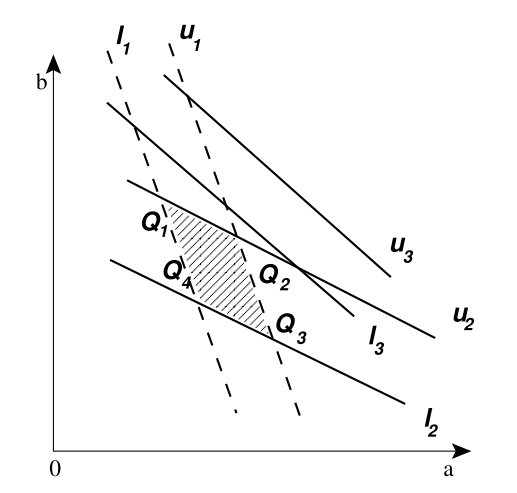
\includegraphics[width=.5\linewidth]{7_11_space.png}\\
  \caption{Feasible coefficient space for quadratic functions}\label{fig:space}
\end{figure}

Recall that the \emph{Adaptive Approximation (AA)} algorithm proposed in the previous paper is based on the technique of segmentation. The basic idea of AA  is to build \emph{Feasible Space (FS)} for the functions' coefficients. For example if we want to approximate two data points $p_0(x_0, y_0)$ and $p_1(x_1, y_1)$ with the second-order polynomial function $y = ax^2 + bx + c$, we can derive that the coefficients $a$ and $b$ must satisfy the following inequalities:
$$y_0 + a(x_1^2-x_0^2) + b(x_1-x_0) \leq y_1 + \delta;$$
$$y_0 + a(x_1^2-x_0^2) + b(x_1-x_0) \leq y_1 - \delta.$$
The coefficient values of $a$ and $b$ are restricted by bounds $l_1$ and $u_1$ as Figure \ref{fig:space} shows. When new data arrives, the algorithm will compute new bounds and intersect the FS with the previous result. If the FS is empty after $p_n$ is added, then the algorithm segments the series at $p_{n-1}$, and then initializes $p_{n-1}$ and $p_n$ as the first two points of the next new segment.

The new contribution of this paper is that it investigates efficient similarity queries on the approximated time series. Specifically, it studies two basic types of similarity queries, i.e., \emph{range queries} and \emph{$k$ nearest neighbor ($k$NN) queries}. In the range query, given a query time series $\tilde{Q}$ and a set of approximated time series $\tilde{\mP}$, it returns every time series in $\tilde{\mP}$ whose distance to $\tilde{Q}$ is less than or equal to $r$. The $k$NN query is defined in a similar way.

The basic idea is to map every approximated time series into a low dimensional space based on the similarity between the approximated time series and a small set of reference time series. It then indexes the similarity values with an R-tree to process similarity searches on the time series efficiently.

The next problem is how to choose the reference time series. When choosing the reference time series, there are two main goals to achieve: 1) The distance from the reference time series to any approximated time series should be computed efficiently; 2) The distance between the reference time series themselves should be large enough. Based on these considerations, the paper proposes to use the following 3 reference time series: $R_1 = (v_{min}, v_{min}, ..., v_{min}), R_2 = (v_{max}, v_{max}, ..., v_{max}), R_3 = (v_{max}, v_{min}, ..., v_{min})$, where $v_{min}$ and $v_{max}$ denote the minimum and maximum values of data points in the time series dataset. These three reference time series represent three corners of the data domain. After the mapping, each approximated time series is represented by a 3-element tuple. The method then uses an R-tree to index the tuples.

When a query is issued, it first maps the query time series to a 3-dimensional point. Then this point is used to perform a search on the R-tree index, which returns a set of approximated time series as the candidate query answers. Finally it checks each candidate answer against the query time series by decompressing them and then computing the exact distance to identify the final query result.

In the experimental section, the new results show the effectiveness of the proposed method on the exchange rate data. It is also shown that in terms of efficiency, the indexing scheme outperforms a scan based search method by at least an order of magnitude in processing $k$NN queries and 40\% in processing range queries.

\section{MASCOT: Fast and Highly Scalable SVM Cross-validation using GPUs and SSDs \cite{WZRQT14}}\label{sec:MASCOT}

This paper proposes a new scheme for scalable and fast \emph{SVM cross-validation} by exploiting the high computation power of GPUs and fast access of SSDs.

\emph{Support Vector Machine (SVM)} is a popular supervised learning model for classification. The training of SVMs is equivalent to solving the following optimization problem:
\[
\max\limits_{\alpha} F(\alpha) = \sum\limits_{i=1}^n - \frac{1}{2} \alpha^T Q \alpha
\]
\[
\mbox{s.t. } 0 \leq \alpha_i \leq C, \forall i \in \{1, ..., n\} \mbox{ and } \sum\limits_{i=1}^n y_i \alpha_i = 0
\]
Here $F(\alpha)$ is the objective function, $\alpha$ is the weight vector, and $Q$ is the matrix computed with the kernel function. The goal of the training is to find $\alpha$ that maximizes the objective function, which can be achieved by the \emph{Sequential Minimal Optimization (SMO)} algorithm  by the following three steps: 1) Search for two extreme examples denoted by $x_u$ and $x_l$. 2) Improve the weights of $x_u$ and $x_l$ (which are $\alpha_u$ and $\alpha_l$ respectively). 3) Update the optimality indicators of all examples.
The $k$-fold cross-validation of a huge dataset by SVM can be expensive, and the paper focuses on how to process the cross-validation by utilizing modern hardwares, specifically the GPUs and SSDs.

Before introducing the proposed technique, its necessary to understand some important features of the GPUs and the SSDs. GPU threads are grouped into \emph{blocks} which further form \emph{grids}. Each thread has its local register (least access latency), each block has share memory (median access latency), and all threads and blocks can access the global memory (large access latency). SSDs are emerging high-performance storage devices. Different blocks of SSDs can be read simultaneously, which significantly accelerates the read speed.

\begin{figure}[h]
  \centering
  % Requires \usepackage{graphicx}
  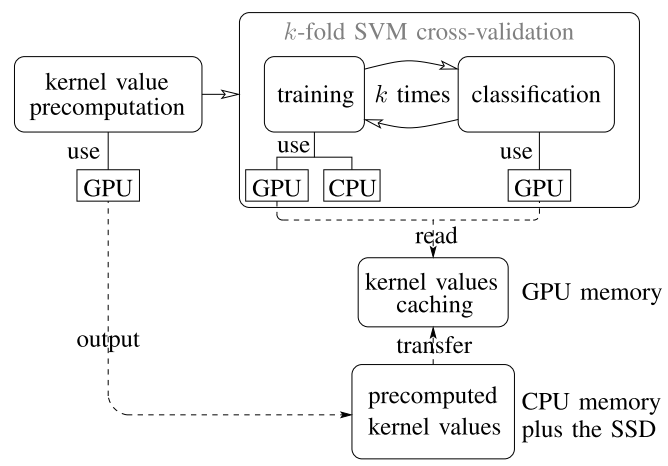
\includegraphics[width=.7\linewidth]{8_8_mascot.png}\\
  \caption{The MASCOT scheme}\label{fig:mascot}
\end{figure}


The paper proposes a scheme called \emph{Modern hArdware enabled Svm CrOss-validaTion (MASCOT)}, for highly scalable and efficient SVM cross-validation (Figure \ref{fig:mascot} shows its main steps). Next we will see the three phases of MASCOT in detail.

The first phase is to precompute, store and obtain kernel values. The kernel matrix is an $n \times n $ matrix that consists of the kernel values of all the examples. The following techniques are applied in this step: 1) It uses GPU to precompute the kernel matrix; 2) The precomputed kernel matrix is stored row after row sequentially in the CPU memory extended by the SSD. The potion of the matrix beyond the CPU memory size is stored in the SSD, and stored in a way that can be read in parallel to make use of SSDs' multi-channel feature. 3) Each training iteration requires two rows, and each classification requires one row. This data is obtained from the precomputed matrix when required.

The second phase is training, which is accelerated by the following techniques: 1) Improving extreme example search. This is achieved by reducing the shared memory consumption (each thread loads a number $m$ of elements instead of one), reducing accesses to the shared memory (each thread maintains its local minimal/maximal value in the register), and early thread termination (after each round of the reduction half threads will be terminated since they will not be used). 2) Caching strategy. Previous studies simply used \emph{least recently used (LRU)} replacement strategy for kernel value caching. The paper shows that this is inefficient, and proposes the \emph{longest access time (LAT)} strategy instead. 3) Distributing tasks on GPUs and CPUs. Some operations are not parallizable, and for these problems CPU's high serial computing capability should be used.

The last phase is the classification step in the cross-validation. There are two ways to read the kernel values: reading all the rows corresponding to the support vectors, or reading all the rows corresponding to the test examples. The algorithm chooses the less rows to read.

In the experimental section, the paper studies the effect of different techniques, and makes comparisons with previous approaches. It is reported that for datasets of sizes that existing algorithms can handle, MASCOT achieves orders of magnitude speedup. More importantly, MASCOT enables SVM cross-validation on datasets of very large scale that existing algorithms are unable to handle.

\section{Processing Moving kNN Queries Using Influential Neighbor Sets \cite{Li0QYZ014}}

This paper revisits the \emph{moving $k$ nearest neighbor (M$k$NN)} query, which is to compute the $k$ nearest neighbor set of a query point and maintain it while the query object is at move. It proposes a new algorithm to process the query efficiently based on the concept of \emph{influential neighbor set}.

\emph{Safe region} is a popular and state-of-the-art technique in processing M$k$NN query. It is a region where the movement of the query object does not cause the current $k$NNs to change. Its details are discussed in paper summary \ref{sec:obs} in this document.

In this paper, instead of using safe regions it uses a small set of \emph{safe guarding objects}, and proves that as long as the current $k$NNs are closer to the query object than the safe guarding objects, the current $k$NNs stay unchanged.

A set of safe guarding objects is called an \emph{influential set (IS)}, in the sense that they are influential in determining whether a $k$NN set is valid. Let $O$ be the set of all objects and $O'$ be the current $k$NN set. Naively $O\backslash O'$ is an IS of $O'$ but using this set to validate the result is inefficient, so the paper tries to find the \emph{minimal influential set (MIS)}. MIS can be obtained by combining the objects corresponding to all neighboring order-$k$ Voronoi cells excluding those already in $O'$.

\begin{figure}[h]
  \centering
  % Requires \usepackage{graphicx}
  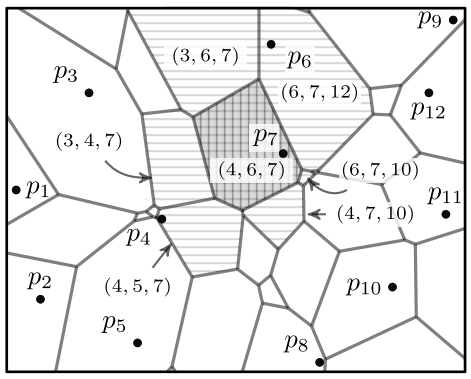
\includegraphics[width=.5\linewidth]{8_8_mis.png}\\
  \caption{The minimal influential set of $O' = \{p_4, p_6, p_7\}$}\label{fig:mis}
\end{figure}


For example suppose $O' = \{p_4, p_6, p_7\}$ as Figure \ref{fig:mis} demonstrates. The union of the neighboring tuples excluding $O'$ is 3, 5, 10, 12. Therefor, the MIS of $O'$ is $MIS(O') = \{p_3, p_5, p_{10}, p_{12}\}$.

To reduce the computational cost, the paper proposes a method to compute an influential set that is slightly larger than the MIS, which is called the \emph{influential neighbor set (INS)}. Specifically, we call an object $p_j$ a Voronoi neighbor of another object $p_i$ if the two Voronoi cells of them share and edge, and all Voronoi neighbors of $p_i$ form its Voronoi neighbor set. Based on this INS is defined to be the union of the Voronoi neighbor sets of all current $k$NNs. The paper formally proves that an INS is an IS.

When an M$k$NN query is issued, the initialization phase computes an initial NN set, denoted by $R$, and the INS of $R$, $I(R)$. The top $k$ objects of $R$ are marked as the $k$NN set ($NN_k(q)$) and $I(R) \cup R \backslash NN_k(q)$ are marked as the IS. Then the query maintenance phase starts. At each timestamp, it checks whether the current $k$NN set is still valid, and updates the result when necessary.

In the experimental section, the paper compares the proposed algorithm with the state-of-the-art algorithm V$^*$-Diagram \cite{NZTK08} in terms of the response time, the number of page accesses and the communication cost. It is reported that the proposed method outperforms V$^*$-Diagram constantly. In some cases the improvement is up to  5 times in page access cost, and 2 times in response time.

\section{Enabling Precision/Recall Preferences for Semi-supervised SVM Training \cite{WZR14}}

There have been many existing work on \emph{semi-supervised learning},  where unlabeled data is used with the labeled data during the learning process. However, those approaches mainly focus on improving the $F_1$ score and cannot express or control precision/recall preferences uniformly. This paper proposes a method that allows to specify a precision/recall preference while maximising the $F_1$ score.

The basic idea is to divide the semi-supervised learning process into multiple rounds of supervised learning. The classifier learned at each round is calibrated according to the precision/recall condition, and then it classifies some of the unlabeled data which is used to enlarge the training dataset.

This paper focuses on the research and implementation on \emph{SVMs}, but the idea is applicable to other learning models such as Bayesian networks and neural networks.
In SVM learning, the precision and recall can be adjusted by the \emph{decision value}, denoted as $\delta$. Specifically after training an SVM classifier, given a new instance $x_l$ the model will label it as $y_l$:
$$
y_l =
\begin{cases}
+1 \mbox{ if } v > \delta\\
-1 \mbox{ otherwise}
\end{cases}
$$
where $v$ is computed according to $x_l$ and the learned SVM model. It is shown in the paper that $\delta$ can control the precision, recall and $F_1$ score: 1) The recall increases when $\delta$ increases; 2) The precision increases when $\delta$ decreases; 3) $F_1$ is maximized when the precision is equal to the recall.

\begin{figure}[h]
  \centering
  % Requires \usepackage{graphicx}
  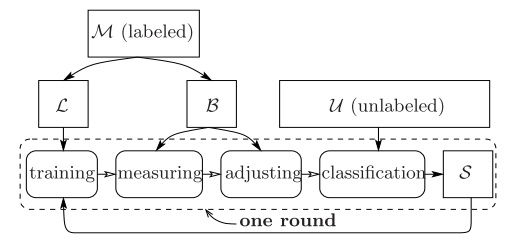
\includegraphics[width=.6\linewidth]{8_8_psvm.png}\\
  \caption{The PSVM method}\label{fig:psvm}
\end{figure}


The key steps of the proposed method, called Preference enabled semi-supervised SVM training (PSVM), are as follows (cf. Figure \ref{fig:psvm}): 1) It randomly divides the labeled dataset $\mM$ into two datasets $\mL$ and $\mB$, where $\mL$ is used as the training dataset and $\mB$ as the calibration dataset. 2) Let $\mT_i$ denote the training dataset, which is initialized as $\mL$. In the $i^{th}$ round, $\mT_i$ is used for training an SVM classifier $\bH$ using the standard supervised SVM training algorithm (all data in $\mT_i$ is always labeled). The calibration dataset $\mB$ is used for measuring the precision and recall of the classifier $\bH$. 3) If the precision (or recall) preference is satisfied, the decision value $\delta$ is adjusted to improve the $F_1$ score. Otherwise the decision value is adjusted to meet the precision (or recall) constraint. 4) The classifier $\bH$ with the adjusted decision values is used for classifying the instances in the unlabeled dataset, which results in a new labeled set $\mS$. Finally $\mS$ is used to enlarge the training dataset, forming $\mT_{i+1}$ in the next iteration.

In the experimental section, the paper makes comparison with the SSVM method (using only $\mM$ as training dataset) and the TSVM method \cite{J99}. It is reported that the proposed PSVM can satisfy a wide range of precision/recall preferences, while the other two alternative approaches have no mechanism to achieve this. Besides, OSVM significantly outperforms SSVM by over 10\% on the $F_1$ score, and constantly outperforms TSVM by three orders of magnitude in terms of efficiency.

\section{Real-time Continuous Intersection Joins over Large Sets of Moving Objects using Graphic Processing Units \cite{WH0Q14}}

The paper proposes a GPU based algorithm called the \emph{Multi-Layered Grid Join (MLG-join)} for the \emph{Continuous Intersection Join query (CI-query)} over moving objects. The algorithm achieves both work and data load balancing across tens-of-thousands of execution threads on GPUs. The paper also presents a cost model for the proposed method, which is used for selecting the optimal parameters.

The CI-query in this paper assumes moving objects with non-zero extents bounded by MBRs. The goal is to return a list of tuples in the form of $\langle a_i, b_j, t_s, t_e \rangle$, meaning objects $a_i$ and $b_j$ intersect during time period $t_s$ to $t_e$. The CI-join query is computed in two phases, generating the initial join pairs (initial join) and then maintaining the results continuously (maintenance).

Most features of GPUs are discussed in the previous paper summary \ref{sec:MASCOT} in this document. Another concept used in the paper is called \emph{coalesced memory access}. It means that consecutive threads are required to request data from consecutive blocks in order to achieve full throughput.

The basic idea of the MLG-join algorithm is to develop a coarse-grained semi-contiguous pruning. The remaining search space consists of blocks of thousands of contiguous comparisons, which are then processed on thousands of GPU threads in parallel with fully coalesced memory access. The MLG-join algorithm processes the query in the following four main steps: \emph{construction}, \emph{probing}, \emph{stream preparation}, and \emph{intersection}.

\begin{figure}[h]
  \centering
  % Requires \usepackage{graphicx}
  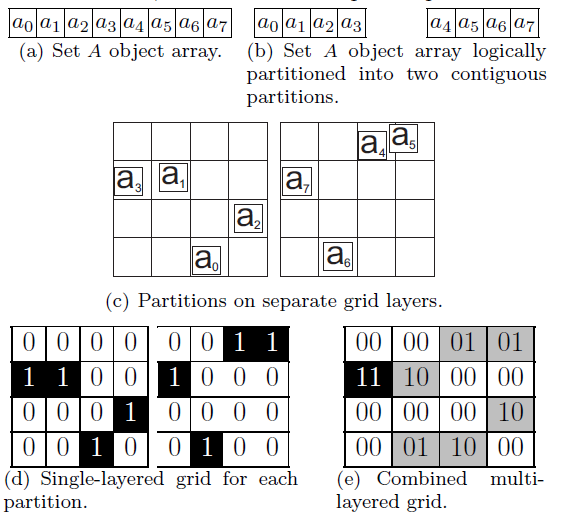
\includegraphics[width=.6\linewidth]{8_8_mlg1.png}\\
  \caption{Constructed multi-layer grid}\label{fig:MLG1}
\end{figure}


In the construction step, the algorithm indexes set $A$ objects using a multi-layered grid. The objects are separated into partitions based on memory locality (location in the sequential array). For example as Figures \ref{fig:MLG1} (a) (b) demonstrate, set $A$ $(a_0,..., a_7)$ is logically partitioned into two parts. In the first part, objects $a_0,...,a_3$ occupy 4 cells as Figure \ref{fig:MLG1} (c) shows. This information is translated to bit representation and combined with the result of the other partitions, as Figures \ref{fig:MLG1} (d) (e) show.

\begin{figure}[h]
  \centering
  \subfigure{
    \label{fig:topka} %% label for first subfigure
    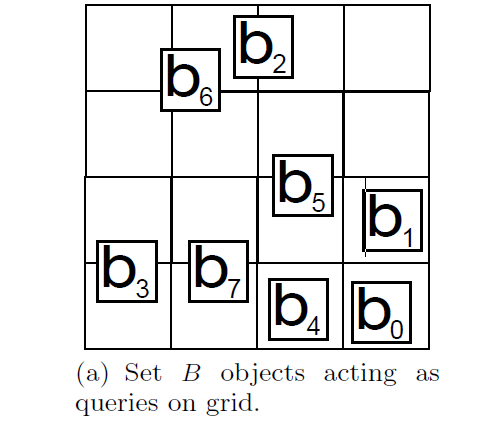
\includegraphics[width=2.2in]{8_8_mlg2.png}}
  \subfigure{
    \label{fig:topkb} %% label for second subfigure
    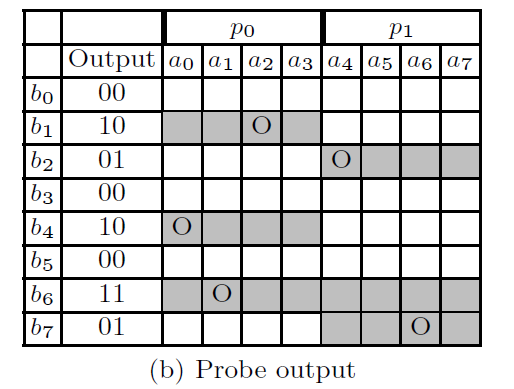
\includegraphics[width=2.2in]{8_8_mlg3.png}}
  \subfigure{
    \label{fig:topkb} %% label for second subfigure
    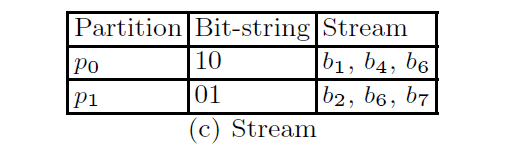
\includegraphics[width=2.2in]{8_8_mlg4.png}}
  \caption{Example of prob and stream preparation}\label{fig:MLG2}
\end{figure}

In the probing step, the algorithm generates a bit-string for every object $b$ in set $B$, where a bit represents whether $b$ intersects at least one object in a partition of set $A$. For example, Figure \ref{fig:MLG2} (b) shows the probing result of the set $B$ objects in (a).

The stream preparation is similar to a \emph{transpose} operation, where the probe output is considered a matrix with a column for each partition and row for each object (cf. Figure \ref{fig:MLG2} (c)).

Finally, the intersection step checks the remaining pairs. It takes into account the precise spatio-temporal location of the objects and checks if an actual intersection occurs.

Then the paper shows that all the four steps can be performed in parallel, and thus leveraging the computing power of GPUs. Take the construction step for example. In the construction step the algorithm assigns threads consecutively to objects in $A$, with one thread per object. The first step is to read the attributes of each object. As the objects in adjacent threads are in adjacent memory locations, the memory access is coalesced. The next step is to calculate which grid cells should be modified, and then write to the grid.% There are many subtle details for the other three steps to be performed in parallel as well, but the discussions are omitted here.

The experimental section verifies the accuracy of the propose cost model, evaluates the effect of the key parameters on the performance, and compares the proposed algorithm with two other alternative approaches. It is reported that the MLG-algorithm outperforms the current state-of-the-art algorithm in all scenarios and by several orders of magnitude.

\section{Efficient Subgraph matching using GPUs \cite{LZWWQ14}}

This paper proposes an efficient GPU-based subgraph matching algorithm and conducts extensive experiments to study the performance.

\begin{figure}[h]
  \centering
  % Requires \usepackage{graphicx}
  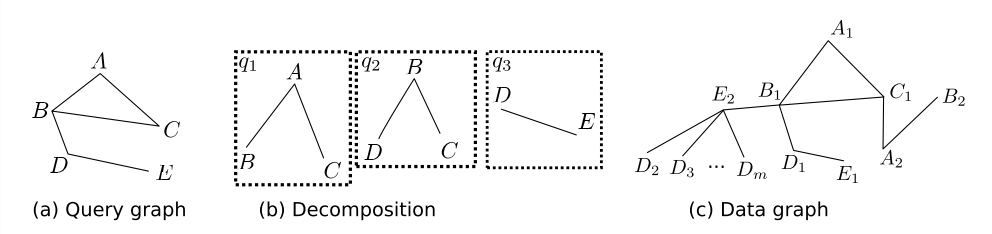
\includegraphics[width=.9\linewidth]{8_1_gpu1.png}\\
  \caption{Example of a query graph and a data graph}\label{fig:gpu1}
\end{figure}


In the subgraph matching problem, a label graph is represented as $G = (V,E,T)$, where $V$ is the vertex set, $E$ is the edge set, and $T$ is a function assigning a label to each vertex. Giving a label query graph $q$, subgraph matching is to find all occurrences of $q$ in $G$. For example the query graph in Figure \ref{fig:gpu1} (a) matches $(A_1, B_1, C_1, D_1, E_1)$ in Figure \ref{fig:gpu1} (c).

The \emph{STwig} algorithm \cite{SWWSL12} can discover matching subgraphs by the following steps. 1) Query graph decomposition: A query graph is decomposed into a set of basic query units called STwigs. For example the query graph in Figure \ref{fig:gpu1} (a) is decomposed to the three STwigs in Figure \ref{fig:gpu1} (b); 2) Matching STwigs in the data graph: Each STwigs matches part of the data graph. Continuing with the above example, the matching result of STwig $q_1$ is $R_1 = \{(A_1, B_1, C_1), (A_2, B_2, C_1)\}$. Similarly the matching results of $q_2$ and $q_3$ are $R_2 = \{(B_1, C_1, D_1)\}$ and $R_3 = \{(D_1, E_1)\}$ respectively; 3) Joining STwig results in the final step: For the example above, the final result set is $R_1\bowtie R_2 \bowtie R_3 =\{(A_1, B_1, C_1, D_1, E_1)\}$.

In this paper the decomposition step and the matching step are performed on the CPU. The GPU-based algorithm is applied in the join step. The basic idea is to make use of hash table to improve  the efficiency.

\begin{figure}[h]
  \centering
  % Requires \usepackage{graphicx}
  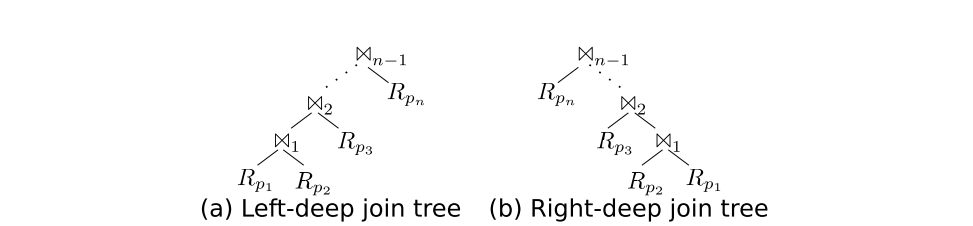
\includegraphics[width=.9\linewidth]{8_1_gpu2.png}\\
  \caption{Two types of join tree}\label{fig:gpu2}
\end{figure}

The first step is to choose a join tree which represents an order of multi-way join. The left child of an internal node is the \emph{build relation}, which means a search data structure (hash table in this paper) will be built for it. The right child is the \emph{probe relation}, whose tuples are used to match with those of the build relation. The paper shows that the right-deep join tree is a better idea (Figure \ref{fig:gpu2} (b)), because a full pipeline mechanism can be used.

The pipeline joining algorithm works like a depth-first search and only a small and fixed amount of intermediate data need to be stored. The basic idea is to ``consume'' the intermediate results as soon as possible. During the join a GPU thread will move forward to process the next subjoin whenever possible, and only moves backward when the current subjoin fails.

The experimental section evaluates the effects of different parameters (data graph size, query graph size, etc.) on the performance. When the proposed method is compared with the CPU-based algorithm, in some cases the improvement is up to an order of magnitude in terms of running time.

\section{Efficient Graph Based Approach to Large Scale Role Engineering \cite{ZR0V14}}

This paper proposes a framework for efficiently identifying administratively beneficial \emph{Role Based Access Control (RBAC)} configurations while ensuring data privacy, called \emph{RoleAnnealing}.

According to the standard notations for RBAC, besides the set of users ($USERS$), roles ($ROLES$), permissions ($PRMS$) and the mappings among them, there is also a partial order on $ROLES$ called the inheritance relation denoted as $\succeq$. $r_1 \succeq r_2$ means that all permissions of $r_2$ are also permissions of $r_1$.

\begin{figure}[h]
  \centering
  % Requires \usepackage{graphicx}
  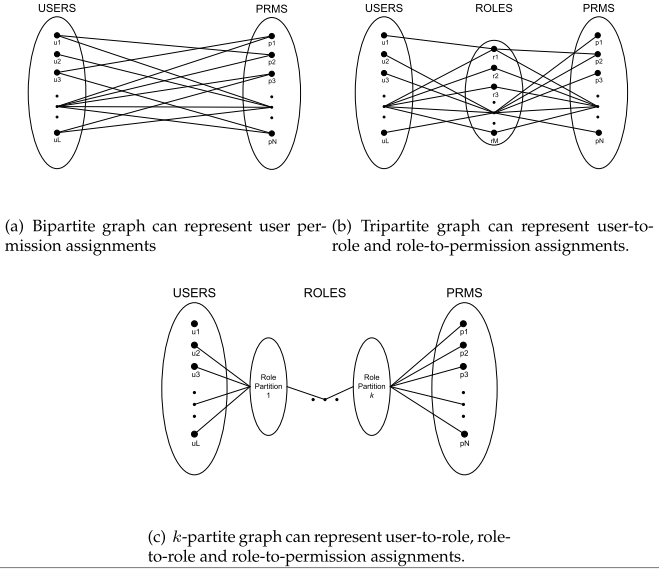
\includegraphics[width=.8\linewidth]{8_1_partite.png}\\
  \caption{$k$-partite graph representations of access control}\label{fig:partite}
\end{figure}

The basic idea is to represent the role engineering problem to a \emph{$k$-partite graph}, allowing for representation of hierarchical roles as well as flat roles. For example, Figure \ref{fig:partite} (a) shows a bipartite graph that represents user permission assignments directly with roles. Similarly, Figure \ref{fig:partite} (b) and (c) show graphs that represent assignments with one layer of roles and multiple hierarchies of roles.

Finding the most administratively beneficial roles is equivalent to finding the RBAC graph with least administrative cost. However, the definition of the cost of a RBAC graph is not that straightforward. The paper proposes two cost models to measured administrative cost.

The first model is called \emph{Role Edge Graph Cost Model}, which focuses on the costs associated with roles and their  role relationships. A graph $G$ is represented as $G = \langle V, E \rangle$, where $V$ is the set of vertices and $E$ is the set of edges. $d^-(v)$, $d^+(v)$ and $d(v)$ denote the in-degree, out-degree and total degree respectively. The cost is defined as:
$$cost(G) = c_1 |V_r| + c_2 |E|.$$
Here $c_1$ is the role cost constant, $c_2$ is the assignment constant, and $|V_r|$ is the number of roles. It also shows how to compute the cost of removing or creating a specific role, which is denoted as $cost(r)$.

The second model is called the \emph{Administration Graph Cost Model}, which focuses on the cost of modifying the graph after RBAC has been implemented. Similarly, the paper presents how to compute the cost of the whole graph ($cost(G)$), and the cost of removing or creating a role ($cost(r)$).

Then the paper proposes a framework, called \emph{RoleAnnealing}, for efficiently identifying administratively beneficial RBAC configurations based on the previously introduced cost model. The basic idea of \emph{RoleAnnealing} is to search for a graph representation that minimizes the cost, and the searching strategy follows the Simulated Annealing algorithm. The paper further develops the following techniques to improve the efficiency. 1) \emph{Incremental computation}: \emph{RoleAnnealing} updates the cost incrementally as a role is removed or created, instead of calculating the graph cost each time; 2) \emph{Guided search}: It guides the search with some hand-crafted rules, such as each created role is assigned to at least two users; 3) \emph{Use of role bounds}: A beneficial role produce a cost reduction ($cost(r)<0$), so a role will be created only if its cost lower bound satisfies the condition; 4) \emph{Separation of create and delete operations}: The search is divided into two conceptual phases. In the first phase only create operations are allowed, and in the second phase only delete operations are allowed.

In the experimental section, the paper studies effectiveness, efficiency and makes comparisons with previous work. It is shown that straightforward implementation requires several orders of magnitude more time than \emph{RoleAnnealing}, and \emph{RoleAnnealing} is also able to identify RBAC configurations of lower cost than the original configurations.

\section{Continuous Visible k Nearest Neighbor Query on Moving Objects \cite{WZXQGY14}}

This paper proposes the \emph{continuous visible $k$ nearest neighbor (CV$k$NN)} query on moving objects, and develops a filtering-and-refinement framework to efficiently process it. It also provides a detailed cost analysis of the proposed method, and validates its accuracy through extensive experiments.

A \emph{visible $k$ nearest neighbor (V$k$NN)} query retrieves $k$ objects that are visible and nearest to the query object. In this paper, it is further assumed that both the query point and data objects are moving, and the goal is to investigate how to retrieve the V$k$NN continuously (i.e., for every timestamp).

The paper proposes a filtering-and-refinement framework to process the CV$k$NN query on moving objects. The framework first performs a two-stage filtering to reduce the search space. Then refinement is performed to examine the exact positions of the objects and find the query result. Next I will explain the first phase in further detail, which is how to prune unpromising objects efficiently.

\begin{figure}[h]
  \centering
  % Requires \usepackage{graphicx}
  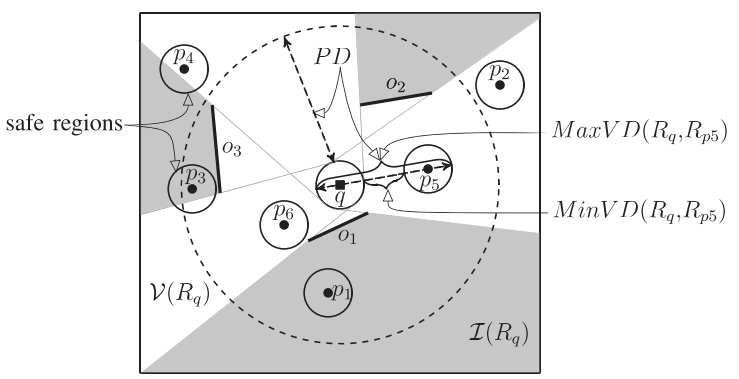
\includegraphics[width=.7\linewidth]{8_1_saferegion.png}\\
  \caption{Safe region based pruning (k=2)}\label{fig:saferegion}
\end{figure}


The first technique is called the \emph{safe region based pruning}. A global maximum speed of all objects is assumed in this paper. With the maximum speed assumption, each object is bounded in its \emph{safe region} during $T$ timestamps. For example in Figure \ref{fig:saferegion}, the safe region of object $p_4$ is the circular region centered at $p_4$. This safe region helps decide if a object is always visible to the query point $q$ during a period of $T$ timestamps. Continuing with the example in Figure \ref{fig:saferegion}, objects $p_2, p_5, p_6$ are always visible to the query point $q$. Suppose $k = 2$, a lower bound distance $PD$ can be derived, and any point whose safe region is farther than $PD$ (for instance $p_2$) can be pruned during the search.

The second proposed technique is called the \emph{invisible time period based pruning}. After the safe region based pruning, there may be some objects whose safe regions are only partially visible to the query point, and with minimum visible distance smaller than $PD$ (for example $p_3$ in Figure \ref{fig:saferegion}). These objects need time to move to be visible, and this time is called the \emph{invisible time period} of $p$, denoted by $\tau_p$. The paper presents a method to compute the lower bound of $\tau_p$, denoted as $\tau_p^l$, such that object can be excluded from examination if current timestamp $t$ is less than $\tau_p^l$. The paper further shows that if the query object's moving direction is taken into consideration, a tighter lower bound $\tau_p^m$ can be achieved. The derivation of the two lower bounds, $\tau_p^l$ and $\tau_p^m$, involve sophisticated mathematics, and the details are omitted here.

In the section of cost analysis, the paper investigates the \emph{communication cost} and the \emph{computational cost}. According to the theoretical result, the combination of safe region pruning and time aware invisible time period based pruning (denoted as SR+MITP) yields the best performance in both metrics.

In the experimental study, the paper evaluates the communication cost and the computational cost while varying different parameters. It is shown that SR+MITP shows the best performance for most cases, and outperforms a naive approach by an order of magnitude in terms of both communication and computational cost, which confirms the aforementioned cost analysis result.

\section{Towards a Painless Index for Spatial Objects \cite{ZQSH14}}

This paper proposes a mapping based spatial indexing scheme called \emph{Size Separation Indexing (SSI)}, and equips it with a suite of techniques including size separation, data distribution transformation, and more efficient mapping algorithms. The paper develops cost model for the proposed structure, based on which the optimal parameter setting can be found. It also shows that SSI can be easily implemented on top of commercial \emph{DBMSs} off-the-shelf, which makes the approach ``painless''.

The first important technique is called \emph{size  separation}. The basic idea is similar to the \emph{size separation spatial join (SSSJ)} method \cite{KS97}, which partitions the objects roughly based on their size using grids of different granularity, and then indexes the objects with \emph{space-filling curves} of different orders. One of the most important difference of the two approaches is that SSI guarantees that the objects are grouped strictly based on their sizes. During this step, one difficulty is to choose a suitable \emph{order} for the space-filling curve for each partition. This paper solves this problem by establishing a cost model to help determining the optimal parameters, the details of which will be discussed later.

The second technique is called \emph{cumulative mapping}, which aims to achieve an approximately uniform distribution for the objects in a partition. For each object $o$ and dimension $j$, SSI defines a mapping $cdf_j(o)$ which returns the percentage of objects whose coordinates are no larger than $o$ in dimension $j$. After this mapping, the data objects will be approximately uniformly distributed. Since obtaining the exact $cdf$ requires sorting all objects which is expensive, the paper further proposes a method to approximate the exact $cdf$ by a \emph{piecewise mapping function (PMF)}.

After cumulative mapping, the objects of each partition are mapped to a space-filling curve to obtain the index keys, and then we only need a classic B$^+$-tree to index the objects from all partitions.

Next let us see how does SSI process window queries. The focus here is how to map a window query to key ranges. First, SSI performs \emph{window query expansion} to guarantee that it does not miss out objects whose centroids lie outside the window query $q$ but intersects it due to extents. Second, it performs the cumulative mapping on the sides of the query window. Finally, the cumulatively mapped window query needs to be further mapped to key ranges based on the space-filling curve using a $MapRange$ function.
The paper proposes two new $MapRange$ algorithms, \emph{EdgeMapRange} and \emph{RoughMapRange}, the details of which are omitted here.

Another contribution of this paper is that it presents a cost model to estimate the number of index page accesses for processing a window query, which is used for choosing the best parameters. First, it supposes that the objects are contiguously indexed (which is not realistic). In this case, the expectation cost of partition $i$ is proved to be $\alpha_i \approx \lfloor \frac{n_q}{C_{max}}\rfloor + \frac{3}{2}$, where $n_q$ is the number of objects and $C_{max}$ is the node capacity of the B$^+$-tree. In the general case, the cost is computed as $\alpha_i \approx p_{cur}(\lfloor\frac{n_q}{C_{max}}\rfloor + \frac{3}{2})$, where $p_{cur}$ is the clustering property of the space-filling curve.

In the experimental study, it is shown that: 1) SSI outperforms other mapping based indexing methods by orders of magnitude. As a standalone implementation, SSI is competitive with the R$^*$-tree. 2) When SSI is implemented on a DBMS, it outperforms the DMBS integrated R-tree by up to three orders of magnitude in processing window queries. 3) The cost model is highly accurate under various settings.

\section{LIMTopic: {A} Framework of Incorporating Link Based Importance into Topic Modeling \cite{DLLZGW14}}

This paper proposes a framework called \emph{LIMTopic} to incorporate link based importance into topic modelling. LIMTopic can be viewed as a generalized framework of the \emph{RankTopic} method \cite{DLLZW12}, which was discussed in a previous paper summary.

Recall that topic modeling aims to represent documents as a distribution over topics instead of words, with the benefit that topics are usually of much lower dimensions and are much more interpretable than words. The motivation of the LIMTopic framework and the RankTopic method is to take advantage of the link structure of a document network since documents have different degrees of importance on different topics.

\begin{figure}[h]
  \centering
  % Requires \usepackage{graphicx}
  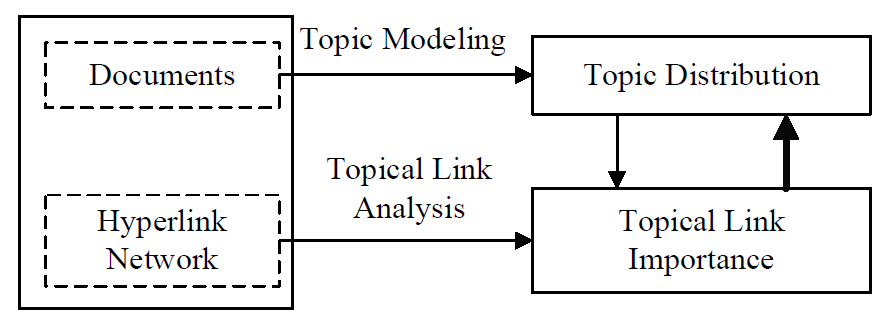
\includegraphics[width=.6\linewidth]{9_5_LIMTopic.png}\\
  \caption{The LIMTopic framework}\label{fig:Topic}
\end{figure}

The LIMTopic framework is illustrated in Figure \ref{fig:Topic}. It can be seen that topical link analysis first performs topic modeling to obtain documents' topic distribution, and then obtains the topical link importance of documents. To incorporate the link importance into topic modeling as the thick line in Figure \ref{fig:Topic} shows is essentially to build the relation between them.

In the LIMTopic framework, topic modeling is achieved by the \emph{PLSA algorithm}, which is the same as the RankTopic method:
Given a collection of $M$ documents $D$, let $V$ be the size of the vocabulary and $K$ be the number of topics. PLSA aims to maximize the likelihood of $D$ with respect to parameters $\Theta$ and $B$:
$$P(D|\Theta,B) = \prod^M_{i=1} \prod^V_{w=1} (\sum_{z=1}^K \theta_{iz} \beta_{zw})^{s_{iw}}.$$
Intuitively, this is a generating model meaning that document $i$ is of topic $z$ with probability $\theta_{iz}$ and topic $z$ generates word $w$ with probability $\beta_{zw}$.

The relation between the topical modeling and topical link importance is also computed in the same way as that of RankTopic: By incorporating topical link importance $\gamma_{zi}$ into the topic modeling, the link information is naturally taken into account. Specifically the likelihood of a collection of documents $D$ is defined as
$$P(D|\gamma, \pi, \phi, \beta) = \prod^M_{i=1} \prod^V_{w=1} (\sum_{z=1}^K [\xi \gamma_{zi} + (1-\xi)\phi_{zi}]\pi_z \beta_{zw})^s_{iw}.$$

The main difference between the LIMTopic framework and the particular RankTopic algorithm is that, in LIMTopic the topic link importance can be different. For example, if the ranking vector is simply taken as the topical link importance computed by the topical pagerank algorithm, the process is exactly the same as RankPage. Other algorithms such as HITS \cite{K99} can also be applied in this step. In this sense, LIMTopic is a more generalized framework.

Finally, the paper derives the logarithm likelihood $L = \log P(D | \gamma, \pi, \phi, \beta)$, and shows how to obtain the local maximum with the \emph{expectation maximization (EM) algorithm}.

In the experimental section, the paper conducts experimental studies of two LIMTopic based models, RankTopic and HITSTopic, and compares them with some state-of-the-art topic models. It is shown that when properly setting the balancing parameter $\xi$, LIMTopic based models perform consistently better than all the other baseline approaches in various aspects, including generalization performance, document clustering and classification, topic interpretability, and document network summarization performance.

\section{Exploiting Transitive Similarity and Temporal Dynamics for Similarity Search in Heterogeneous Information Networks \cite{HBZ14}}

This paper studies the problem of \emph{similarity search} in \emph{heterogeneous information networks} and proposes an improved meta path-based similarity measure which incorporates \emph{transitive similarity} and \emph{temporal information}.

Different from \emph{homogeneous information networks}, which only consider one type of objects and links, heterogeneous information networks involve multiple types of objects and links. For example, heterogeneous bibliographic networks contain authors as well as other types of objects, such as papers, venues, and terms in the paper title. This paper focuses on the problem of similarity search in heterogeneous networks, aiming to discover the most relevant objects with respect to a given query object.

The concept of \emph{network schema} \cite{SHYYW11} has been proposed to describe the meta structure of a heterogeneous network. It is a graph defined as $S_G = (\mathcal{T}, \mathcal{R})$ where $\mathcal{T}$ is the set of object types and $\mathcal{R}$ is the set of link types. A \emph{meta path} $\mathcal{P}$ is a path defined over network schema. For example, Figure \ref{fig:schema} (a) shows a bibliographic network schema, (b) shows a meta path ``author-paper-venue-paper-author'' (\emph{APCPA}) describing authors who publish papers in the same conferences, and similarly (c) shows meta path \emph{APA} describing co-author relationship.

\begin{figure}[h]
  \centering
  % Requires \usepackage{graphicx}
  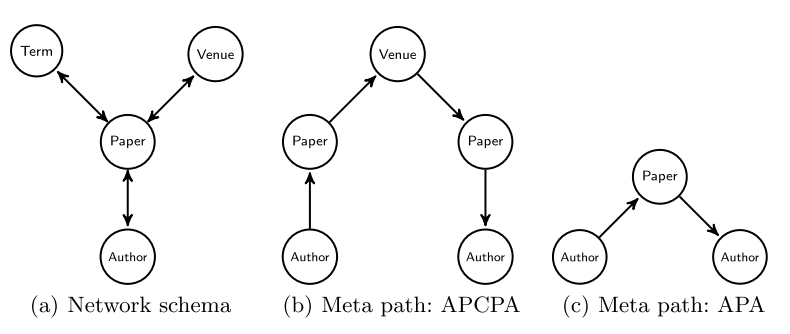
\includegraphics[width=.7\linewidth]{8_1_schema.png}\\
  \caption{An example of network schema and meta paths}\label{fig:schema}
\end{figure}


\emph{PathSim} \cite{SHYYW11} is a meta path-based similarity measure, which computes the similarity between $x$ and $y$ for a given meta path $\mathcal{P}$ as
$$s(x,y) = \frac{2 \times | \mathcal{P}_{x \rightsquigarrow y} |}{| \mathcal{P}_{x \rightsquigarrow x} | + | \mathcal{P}_{y \rightsquigarrow y} |},$$
where $| \mathcal{P}_{x \rightsquigarrow y} |$ is the set of paths between $x$ and $y$, and $| \mathcal{P}_{x \rightsquigarrow x} |$ and $| \mathcal{P}_{y \rightsquigarrow y} |$ are similar. Let $\mathcal{P} = T_1T_2...T_l$ (where $T_i$s are object types), $| \mathcal{P}_{x \rightsquigarrow y} |$ can be computed through the commuting matrix $M$. Specifically $M = W_{T_1T_2}W_{T_2T_3}...W_{T_{l-1}}W_{T_l}$, where $W_{T_iT_j}$ is the adjacent matric between type $T_i$ and $T_j$. Once $M$ is computed, we have $M_{xy} = | \mathcal{P}_{x \rightsquigarrow y} |$.

The basic idea of this paper is to extend \emph{PathSim} by incorporating transitive similarity and temporal information.

In introducing transitive similarity, a meta path is first decomposed to a set of sub paths, formally $\mathcal{P} = \mathcal{P}_1 ... \mathcal{P}_d$. For example, a meta path \emph{APAPA} is decomposed to \emph{APA} and \emph{APA}. In this paper, the commuting matrix of $\mathcal{P}$ is computed as
$$M_{\mathcal{P}} = M_{\mathcal{P}_1}^s M_{\mathcal{P}_2}^s... M_{\mathcal{P}_{d+1}}^s,$$
where $M_{\mathcal{P}_i}^s$ is the commuting matrix for sub path $\mathcal{P}_i$ with transitive similarity incorporated. Formally
$$M_{\mathcal{P}_i}^s = M_{\mathcal{P}_i} \cdot S_{\mathcal{P}'},$$
where $S_{\mathcal{P}'}$ denotes a transitive similarity matrix computed on some other possible path $\mathcal{P}'$.

In the second technique, temporal information is taken into account. The basic intuition is that two objects are more similar if there are more recent connections between them. The method puts different weights on the paths formed in different timestamps. Essentially, the older paths make less contribution to similarity than recent ones, and should be given lower weights. The method to achieve this idea is also to modify the commuting matrix $M_{\mathcal{P}_i}$ to $M_{\mathcal{P}_i} \cdot Y_{\mathcal{P}_i}$, and the details are omitted here.

In the experimental section, the proposed method is evaluated based on the assumption that similar objects will show similar behavior in some way in the future. Specifically the method is evaluated on the DBLP dataset by predicting co-author relationships in the future. It is reported that after incorporating the transitive similarity the accuracy is improved by up to 4\%. If both transitive similarity and temporal information are incorporated, the improvement is up to 15\%.

\section{MELODY-Join: Efficient Earth Mover's Distance Similarity Join Using MapReduce \cite{HZBC14}}

This paper proposes a novel framework named \emph{Mapreduce Earth mover's distance Lower bOund baseD similaritY Join (MELODY-JOIN)} for processing the \emph{Earth Mover's Distance (EMD) similarity join}. The proposed parallel computation paradigm has enhanced pruning power and addresses the load balancing problem.

In this paper a data object (an image for example) is represented as a histogram $h$ that has $n$ bins. Each bin consists of a location vector $\vec{l_i}$ and a weight $w_i$. The EMD between a pair of histograms is the minimum cost of transforming one to the other. The EMD similarity join retrieves all pairs of histograms $h_R$ and $h_S$ such that their EMD, denoted as $EMD(h_R, h_S)$, is not larger than a given threshold $\epsilon$.

The basic idea to improve efficiency is to make use of lower bounds of EMD, since any pairs with a lower bound larger than $\epsilon$ can be discarded. In a previous work the \emph{normal lower bound of EMD (normal LB)} \cite{RS11} was introduced, and this paper also employs it to prune dissimilar pairs in MELODY-JOIN.

\begin{figure}[h]
  \centering
  \subfigure[A 2D histogram]{
    \label{fig:topka} %% label for first subfigure
    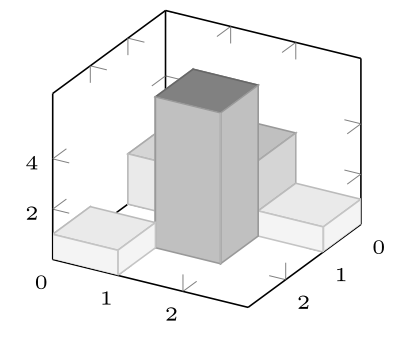
\includegraphics[width=1.4in]{7_25_melody1.png}}
  \subfigure[Normalized projected 1D histogram]{
    \label{fig:topkb} %% label for second subfigure
    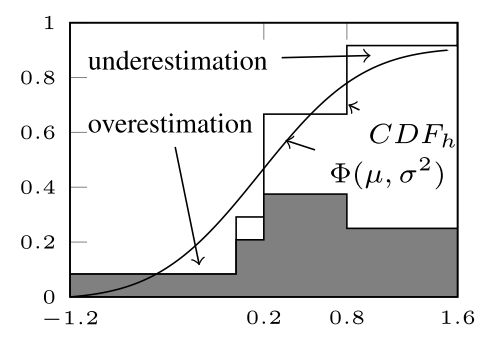
\includegraphics[width=1.4in]{7_25_melody2.png}}
  \subfigure[Grouped records for computing the normal LB]{
    \label{fig:topkc} %% label for second subfigure
    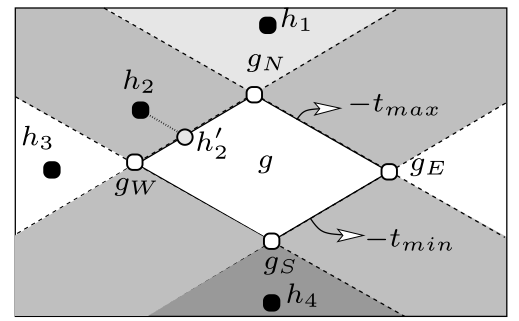
\includegraphics[width=1.4in]{7_25_melody3.png}}
  \caption{Example of computing the normal LB}\label{fig:melody}
\end{figure}

The normal LB between a histogram and a group of histograms is obtained and used by the following steps: 1) Projecting the original histograms to one-dimensional histograms. For example a two-dimensional histogram shown in Figure \ref{fig:melody} (a) will be projected to a one-dimensional histogram as shown in Figure \ref{fig:melody} (b). 2) Constructing \emph{Cumulative Distribution Function (CDF)} for the one-dimensional histograms, approximating the CDF with a normal distribution and transform it to \emph{Hough normal space}, as Figure \ref{fig:melody} (b)(c) show. 3) Grouping the transformed records into diamond-shape region. It was proved that for each transform record $h$ and a region $g$, the EMD between $h$ and any $h_g \in g$ is at least greater than the computed normal bound ($EMD(h, h_g \in g) \geq LB_{normal}(h,g))$, which means that normal LB is indeed a useful lower bound.

Based on the idea of normal LB, the proposed MELODY-JOIN involves three MapReduce jobs as follows: 1) Job 1: Obtaining the domain of transformed space. 2) Job 2: Computing the approximation errors for cells, which are used for computing the normal LB between a record and a cell. 3) Pruning, partitioning and refining records, and producing the final join results.

There are two key performance issues in MELODY-JOIN: the limited pruning power of a single normal LB, and the unbalanced workloads on reducers in Job 3. The paper proposes several techniques to address these two issues. 1) Multiple lower bounds are employed at the same time. It can use multiple projection vectors to produce multiple Hough normal spaces and pruned the data with multiple normal LBs. Alternative lower bounds may be used as well. 2) The quantile values in each dimension of the Hough normal space are used to divide the space into a quantile based grid, such that the grid cells contain more balanced numbers of records.

In the experimental section, the paper evaluates the performance of the proposed method while varying different parameters, and makes comparison with a baseline method. It is shown that MELODY-JOIN consistently outperforms the baseline algorithm by an order of magnitude, and it also scales up well while the data size or the number of computing nodes increases.

\section{The Min-dist Location Selection and Facility Replacement Queries \cite{QZWXYK14}}

This article is an extended version of a previous paper \cite{QZKLX12}. The previous paper proposes and studies a new type of location optimization problem, called the \emph{min-dist location selection problem}. This paper also investigates a variant of the problem called the \emph{min-dist facility replacement problem}. It also provides a detailed comparative cost analysis and conducts extensive experiments on the various algorithms.

Recalled that the min-dist location selection problem is defined as follows. Given a set of clients $C$ and a set of existing facilities $F$, it selects a location from a given set of potential locations for establishing a new facility, so that the average distance between a client and her nearest facility is minimized.

The first observation is that the min-dist query can be reduced to a simpler form. We call the distance between a client and her nearest facility the \emph{nearest facility distance (NFD)}. Given a location $o$, the \emph{influence set} of $o$ (denoted as $IS(o)$) is the set of clients that can get NFD reduction if a new facility is built there. The min-dist query is to minimize the sum of all clients' NFD. If a new facility $p$ is established, the sum of all clients' NFD will decrease, and we call it the \emph{distance reduction} of $p$ and denote it as $dr(p)$. So the min-dist query is equivalent to finding a potential facility $p$ with maximal $dr(p)$.

In the previous paper, besides a naive sequential scan method, it proposes three algorithms for processing the min-dist location selection queries. The first proposed technique is called the \emph{quasi-Voronoi cell (QVC) method}, which prunes search by forming a QVC for each potential location $p$ such that any customer outside the QVC cannot be influenced by $p$. The second technique exploits the concept of \emph{nearest facility circle (NFC)} and is called the NFC method. Since both QVC and NFC methods have their advantages and drawbacks, the previous paper further develops the \emph{maximum NFC distance (MND) method}.

The main new contribution of this paper is that it proposes a variant of the problem called the min-dist facility replacement problem where it considers replacing (instead of adding) a facility while achieving the same optimization goal. The paper introduces two algorithms for processing the query.

The first algorithm is based on the concept of clients' \emph{second nearest facility circles (SNFC)}, which are circles of clients' second nearest facilities, so the resultant method is called the \emph{maximum SNFC distance (MSND) method}. Similarly to the MND method, the first step is to represent the problem to a simpler form. Let $dr(\langle f, p \rangle)$ be the distance reduction if $f$ and $p$ are selected for the replacement. The min-dist facility replacement problem is equivalent to finding a pair of $f$ and $p$ that maximize $dr(\langle f, p \rangle)$. The basic idea of MSND is based on the observation that when $f$ is replaced by $p$, the nearest facility of a client $c$ may stay unchanged, or become either $p$ or the existing SNF of $c$. So the algorithm analyzes different cases of the computation of the distance reduction $dr(\langle f, p \rangle)$. Then it applies the technique used in the MND method to build an R-tree variant to index the clients and bounding regions for their NFCs as well as SNFCs. When it performs a range query for every pair of facility and location, this index structure can efficient find all the relevant clients.

The MSND method reduces the search space from $F \times P \times C$ to $F \times P \times \tilde{C}$, where $\tilde{C}$ is a subset of $C$. This is a search cubically proportional to the size of the datasets. The next technique aims to replace a cubical search with two lightweight quadratic searches plus a lightweight cubical search.

The second algorithm uses a concept called the \emph{Replacement Influence Distance (RID)} to help identify the facility-location pairs that require $dr$ value aggregation, so the resultant method is called the RID method. The motivation behind the RID method is that, instead of considering a pair $\langle f, p \rangle$ as a unit, it considers it as two independent pairs and computes $dr(f)$ and $dr(p)$ separately. In this way, it can apply the MND method to efficiently compute $dr(f)$ and $dr(p)$ (two lightweight quadratic search), and only pair up the promising facilities and potential locations to find the optimal pair.

In the experimental section, the new results show that RID constantly outperforms \emph{SS-FR} (where the facilities, potential locations and clients are sequentially scanned for $dr$ value computation) and MSND under various setting by up to five orders of magnitude.

\section{Traffic Information Publication with Privacy Preservation \cite{GLJHZ14}}

This paper aims to solve the problem of publishing traffic information without violating each user's location privacy concerns. It identifies a new privacy problem called the inference-route problem, and proposes an efficient and effective clustering-based anonymization algorithm.

\begin{figure}[h]
  \centering
  % Requires \usepackage{graphicx}
  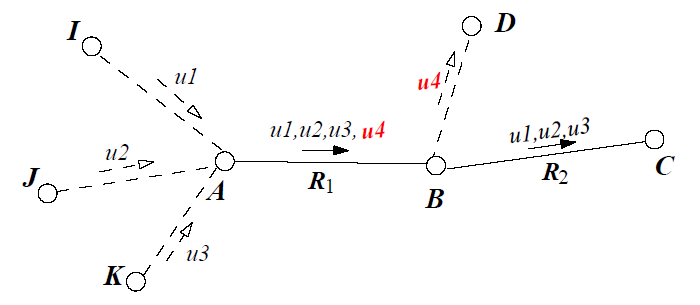
\includegraphics[width=.5\linewidth]{9_5_pub.png}\\
  \caption{An example of inference-route problem}\label{fig:pub}
\end{figure}

The goal of the study is to prevent adversaries from mapping published locations to a specific individual. For example Figure \ref{fig:pub} shows three users $u_1, u_2$ and $u_3$ with their trajectories respectively. In general, raw data is represented as a tuple $\langle ID, loc, vel, t \rangle$, where $ID$ is the object ID, $loc$ and $vel$ are object location and velocity at timestamp $t$. For example the raw data of user $u_1$ is composed of four tuples: $\langle u_1, I, vel_1, t_1 \rangle, ..., \langle u_1, C, vel_4, t_4 \rangle$. In order to protect individual privacy, when publishing the traffic data it is desirable to only publish the information of popular trajectory segments, such as the edegs $R_1$ and $R_2$.

In this paper the proposed approach has three main properties: 1) It guarantees \emph{$k$-anonymity} of published data, which means for each published trajectory segment there are at least $k$ vehicles pass by. 2) It avoids the \emph{inference-route problem}. The inference-route problem can also be explained by Figure \ref{fig:pub}. Suppose all the users in routes $R_1$ and $R_2$ are reported, an adversary can easily deduced the private trajectory of user $u_4$ on road $BD$, although this is not revealed in the data. 3) The anonymization results follow the road-network constraints.

The method has two main steps. First, it partitions the time into intervals, and groups records within the same interval. In each obtained sub-dataset, it removes records with infrequent roads (roads with less than $k$ objects visited). The second step is the core of the process. The paper proposes a clustering-based algorithm that produces the result.

The essential idea of the clustering-based anonymization algorithm is to find clusters of similar trajectories and anonymize them by using a representative trajectory. Specifically, the trajectories are arranged in a descending order of their supports, which is defined as the number of users who have the same trajectories. For the remaining trajectories, the algorithm compares it with existing clusters. If there exists a suitable cluster, the new trajectory is inserted into it. Otherwise, a new cluster will be created.

\begin{figure}[h]
  \centering
  % Requires \usepackage{graphicx}
  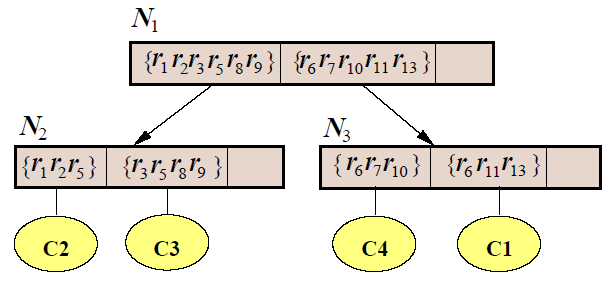
\includegraphics[width=.5\linewidth]{9_5_Ctree.png}\\
  \caption{An example C-tree}\label{fig:Ctree}
\end{figure}

To further improve the efficiency of the process, a data structure called \emph{C-tree (Cluster-tree)} is proposed (cf. Figure \ref{fig:Ctree}). In leaf nodes, each entry has a pointer to a cluster and the IDs of roads occurring in that cluster. In internal nodes, each entry has a pointer to a child node and the union of road IDs in the child node. For example when it needs to find the cluster of a new trajectory $r_2 r_4$, the algorithms checks the similarity of it with two internal entries in $N_1$. If the similarity w.r.t. some entry is above a threshold, the algorithm continues to visit the child node and repeats the process. With this method, all candidate clusters can be efficiently retrieved. Finally among all candidate clusters, the algorithm calculates the edit distances between the representative trajectories and the new trajectory. Based on the edit distance, a local error is computed, and the new trajectory is clustered with the one with the smallest local error.

In the experimental section, the performance of the proposed method is evaluated based on five criteria: 1) anonymization time; 2) average error rate; 3) standard deviation; 4) number of inference-routes in the result; 5) number of frequent patterns after anoymization. The experimental results show that the proposed method outperforms the latest related work in terms of both efficiency and effectiveness.

\section{DesTeller: {A} System for Destination Prediction Based on Trajectories with Privacy Protection \cite{XZZXYTJZ13}}

This article is based on a previous paper \cite{XZZXHX13}, in which an algorithm called \emph{Sub-Trajectory Synthesis (SubSyn)} is proposed to solve the destination prediction problem. This paper showcases a system named ``\emph{DesTeller}'', which uses SubSyn as its underlying algorithm.

Recalled that the main difficulty is destination is the ``data sparsity problem'', i.e., the available historical trajectories are far from being able to cover all possible trajectories. The basic idea of SubSyn is to use the \emph{Bayesian inference framework}, and uses a \emph{first order Markov model} to efficiently compute the posterior probability for any trajectory. The previous paper also introduces a method to protect privacy against the SubSyn algorithm. The privacy protecting techniques aim to make the destination probability of a private location lower than a chosen threshold.

\begin{figure}
  \centering
  % Requires \usepackage{graphicx}
  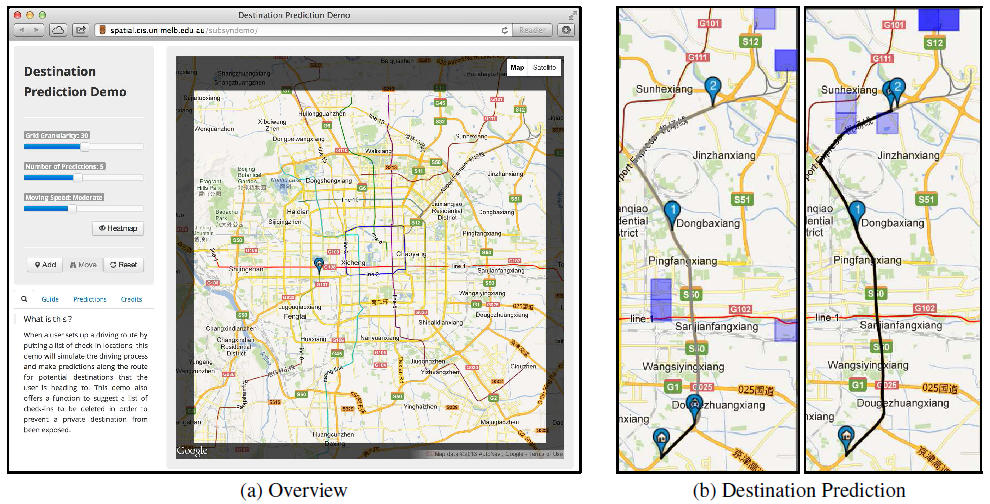
\includegraphics[width=\linewidth]{9_5_desA.png}\\
  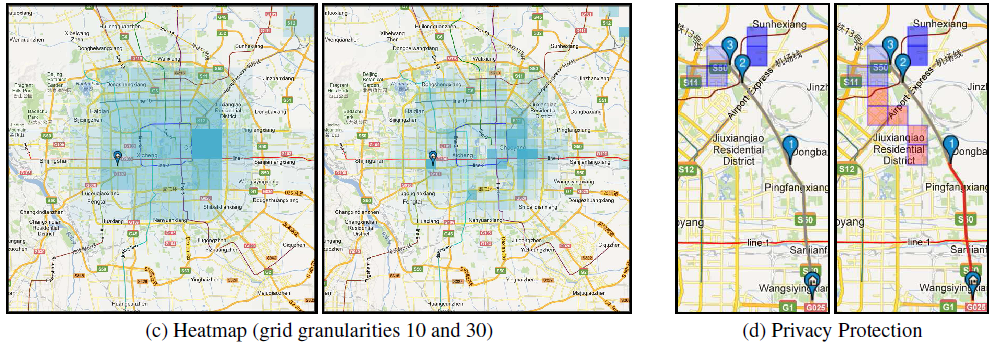
\includegraphics[width=\linewidth]{9_5_desB.png}\\
  \caption{Screenshots of the Demonstration System}\label{fig:des}
\end{figure}

The new contribution of this paper is that it presents the demonstration program (DesTeller), and describes use cases and scenarios of its application. Firstly, a screenshot of the demonstration program is shown in Figure \ref{fig:des} (a), which illustrates DesTeller in the form of a webpage. It also offers an option named heatmap (cf. Figure \ref{fig:des} (c)) to reveal all popular destinations in Beijing. In the following paragraphs, I will present two use cases of DesTeller.

The first use case corresponds to Figure \ref{fig:des} (b). Consider a user, John, was driving from his hotel (bottom left corner) to the airport (top right corner). Soon after he left the hotel, the GPS recommended several likely destinations (blue squares in left Figure \ref{fig:des}) including the airport. John selected the airport from the list without manually searching it. During his entire trip, the system continued to predict destinations and sent recommendations to him.

The second use case is shown in Figure \ref{fig:des} (d). Consider the following scenario in which a user called Jane takes advantage of the privacy protection solution to avoid privacy leak. Jane has a geo-social application on her smartphone, and during an afternoon she was on he way home from a public event. Right before arriving at her house, four locations are recorded from auto check-ins. Since the privacy protection solution is in place, before publishing each location, Jane received a confirmation dialogue showing a list of predicted destinations (blue squares) if the locations were published. Instructed by Jane, the program processed the privacy protection request, and returned a new list of locations which were the results of deleting the smallest number of locations such that her true destination is not revealed.

\section{Destination Prediction by Sub-Trajectory Synthesis and Privacy Protection Against Such Prediction \cite{XZZXHX13}}

This paper identifies the \emph{data sparsity problem} in \emph{destination prediction} and proposes a novel \emph{Sub-Trajectory Synthesis (SubSyn)} algorithm to address this problem. It also takes into account the \emph{privacy protection} issue in case an adversary uses the SubSyn algorithm to derive sensitive location information of users.

\begin{figure}[h]
  \centering
  % Requires \usepackage{graphicx}
  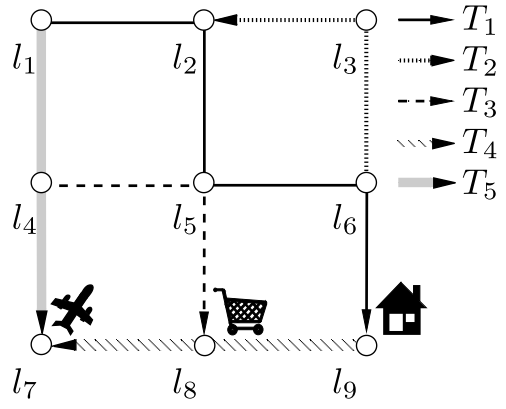
\includegraphics[width=.6\linewidth]{7_25_dest_pred.png}\\
  \caption{An example of destination prediction}\label{fig:dest}
\end{figure}


Figure \ref{fig:dest} presents an example destination prediction problem. There are five historical trajectories $T_1, ..., T_5$, and each of them is represented by a different type of line. Suppose that now a client is moving from $l_1$ to $l_4$, and this query trajectory partially matches $T_5$. Therefore, the destination of $T_5$ (i.e. $l_7$) is the predicted destination of the query trajectory.

However, existing approaches suffer from the ``data sparsity problem'', i.e., the available historical trajectories is far from being able to cover all possible trajectories. For example, if the query trajectory is $\{l_1, l_4, l_5\}$, existing approaches will fail to return a result since no historical partially matches the query.

The basic idea of the proposed SubSyn algorithm is based on the \emph{Bayesian inference framework}. Intuitively, the probability of a node $n_j$ being the destination can be computed as the probability that the destination location $d$ is in $n_j$ ($d \in n_j$), conditioning on the query trajectory $T^P$. Formally the probability is computed as
$$P(d\in n_j | T^P) = \frac{P(T^P|d \in n_j)P(d\in n_j)}{\sum\limits^{n_k}_{1 \leq k \leq g^2} P(T^P|d\in n_k)P(d\in n_k)}.$$
Here the \emph{prior probability} $P(d \in n_j)$ can be easily computed as the number of trajectories  terminating at $n_j$ divided by the total number of trajectories. Next I will explain how to compute the \emph{posterior probability} $P(T^P | d \in n_j)$ by the SubSyn approach.

SubSyn uses a \emph{Markov model} to efficiently compute the posterior probability for any given trajectory online. Intuitively, the \emph{first order Markov assumption} implies that the probability of the next location only depends on the current position. The paper first defines the concept of \emph{total transition probability} $p_{i \rightarrow k}$, which is the probability of all possible paths between $n_i$ and $n_k$ in certain steps. A method based on matrices multiplication is proposed to compute the total transition probabilities efficiently. Then it shows that the posterior probability can be computed as
$$P(T^p | d \in n_j) = \frac{P(T^p) \cdot p_{c \rightarrow j}}{p_{s \rightarrow j}}.$$
Here $P(T^p)$ us the path probability of the given partial trajectory query $T^p$, which is defined as
$$P(T^p) = P(T_{1,2,...,k}^p) = \prod \limits^k_{i=1} p_{i(i+1)}.$$

The paper also introduces a method to protect privacy against the SubSyn algorithm. The privacy protecting techniques aim to make the destination probability of a private location lower than a chosen threshold $k$, through deleting the smallest number of nodes from the query trajectory. The first naive solution is called the \emph{Exhaustive Generation Method}. Its basic idea is to iteratively delete one node from the given partial trajectory, until the privacy condition is satisfied. The second proposed approach is called the \emph{End-Points Generation Method}, which is much more efficient than the first naive approach. The end-points generation method makes use of the fact that under the first order Markov assumption, the probability of any potential destination depends only on the starting node $n_s$ and the most recent node $n_c$ in the trajectory. So when iteratively removing a node from the candidate trajectory, the algorithm only need to try the options of deleting two end points.

In the experimental section, the paper mainly studies the effectiveness and efficiency of the proposed method, and compares the result with the \emph{ZMDB} algorithm \cite{ZMDB08}. It is reported that SubSyn can predict up to ten times more query trajectories than the baseline algorithm, and runs over two orders of magnitude faster than it. It is also shown that the advanced privacy protecting algorithm runs more than two orders of magnitude faster than the naive approach.


\section{Feel Free to Check-in: Privacy Alert against Hidden Location Inference Attacks in GeoSNs \cite{HMZ13}}

This paper proposes a new privacy attack called \emph{hidden location inference attack}, and develops three inference models to accurately derive the \emph{hidden location leakage probability (HLPL-probability)}. It also designs a privacy alert framework to warn users the most probable leaked hidden locations.

In the proposed problem, people are using check-in service in \emph{Geo-Social Network (GeoSN)}, and a user can report publicly which \emph{points of interest (POI)} she has visited. In such scenarios, hidden location inference attack is a kind of location privacy attacks, from which adversaries can infer users' most probable visited hidden locations.

\begin{figure}[h]
  \centering
  % Requires \usepackage{graphicx}
  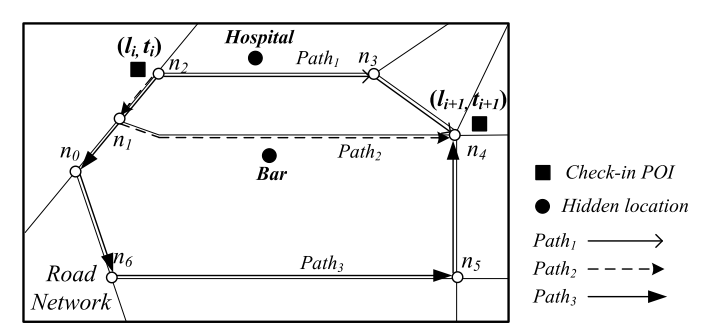
\includegraphics[width=.6\linewidth]{7_25_checkin.png}\\
  \caption{An example of hidden location privacy leakage}\label{fig:checkin}
\end{figure}

For example in Figure \ref{fig:checkin}, a user $u_k$ checks in POI $l_i, l_{i+1}$ at time $t_i, t_{i+1}$ respectively. Since the road network is publicly accessible, adversaries know that $u_k$ might have taken one of the three paths $Path_1, Path_2$ and $Path_3$. Suppose there is a hospital and a bar on $Path_1$ and $Path_2$. Although $u_k$ did not check in at these two locations for fear of privacy leakage, adversaries may infer how likely she visited one of them. Next I will explain the three inference models proposed in this paper.

In the first \emph{baseline inference model}, adversaries can use the majority users' behavioral patterns to ``guess'' how likely one would visit a POI. Given a hidden location $l_m$ and the time interval between two check-ins $\Delta t$, the HLPL-probability can be denoted as a posterior probability $P(V_k^{i,m,i+1} | \Delta t)$, and this can be computed by the Bayes' Law. Furthermore, this probabilistic model can be introduced a parameter called \emph{friend closeness}, with which friends with similar behaviors will have more influences.

The second inference model is called the \emph{collaborative filtering (CF) based inference model}. Its basic idea is similar to the \emph{collaborative filtering} technique which is widely applied in the recommender systems: In GeoSNs, similar users who might share a lot of common interests tend to have similar visit behaviors, according to which the HLPL-probability can be inferred. Specifically, the method utilizes two matrices to calculate a user's visit probability to hidden locations. Matrix $S$ is a user-user matrix, which represents the similarity between users. Matrix $U$ is a user-location matrix, which represents the visit probability of each location for each user. The CF method completes matrix $U$ through iterations, until the two matrices converge.

The final approach is named the \emph{hidden Markov model (HMM) based inference model}. Given a user $u_k$ whose hidden locations are being analyzed, the observed nodes are the check in locations of $u_k$'s friends and her similar users. The hidden nodes are the corresponding hidden locations that $u_k$ might visit. The HMM model is trained by the \emph{Expectation-Maximization (EM) algorithm}, with which the probability of the hidden nodes can be derived by the observations.

\begin{figure}[h]
  \centering
  % Requires \usepackage{graphicx}
  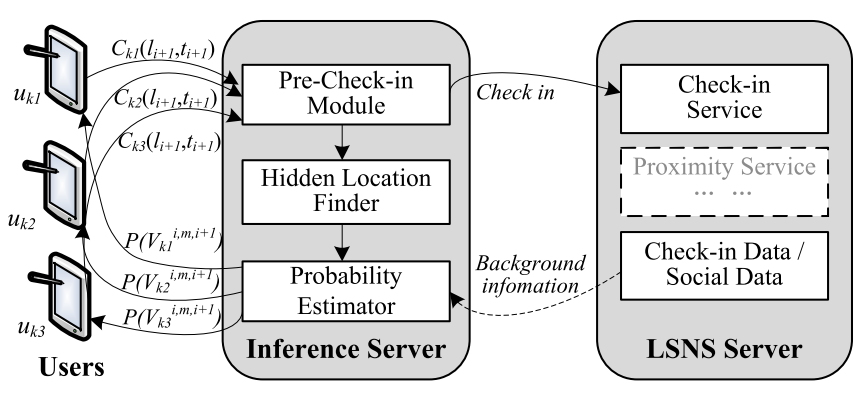
\includegraphics[width=.6\linewidth]{7_25_checkin_system.png}\\
  \caption{System architecture}\label{fig:checkin_system}
\end{figure}

Finally, the paper introduces a hidden location privacy inference framework based on the \emph{client-inference server-GeoSN server} model as depicted in Figure \ref{fig:checkin_system}. In the inference server, hidden location finder finds out all the hidden locations for each user, and then probability estimator evaluates users' HLPL-probabilities with the inference models previously introduced. During the process, necessary background information is acquired from the GeoSN server. At last, the most probable leaked hidden locations are pushed to users as a privacy alert.

In the experimental study, the paper evaluates the effectiveness and efficiency of the proposed method. It is shown that the HMM-based inference model always exhibits the best performance in terms of accuracy. The average response time is in minutes level. Although the response time does not satisfy the real-time applications, the framework is still available since the response time is much shorter than users' average stay time at a place.

\section{Countering Overlapping Rectangle Privacy Attack for Moving kNN Queries \cite{HKZ13}}

This paper identifies the overlapping rectangle attack in a \emph{moving $k$ nearest neighbor (M$k$NN)} query and develops a technique called \emph{Confidence Level Aware Privacy Protection In Nearest Neighbor Queries (CLAPPINQ)} to overcome this attack.

In a M$k$NN query, a moving client continuously sends requests to a \emph{location-based service provider (LSP)} for $k$ nearest location objects (gas stations, hospitals, etc.). A popular technique to protect a user's privacy from the LSP is called \emph{obfuscation}, which sends a rectangle region that includes the user's exact location to the LSP. However, the paper shows that the LSP can still approximate the user's location by the overlapping rectangle privacy attack and the maximum movement bound attack.

\begin{figure}
  \centering
  % Requires \usepackage{graphicx}
  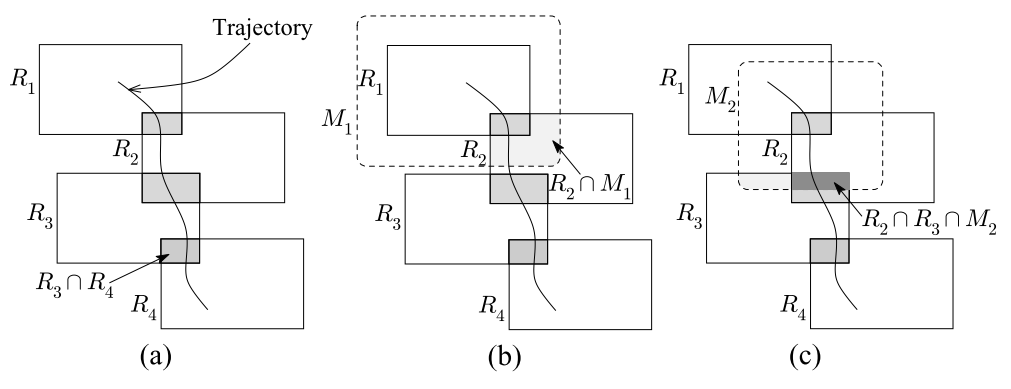
\includegraphics[width=.9\linewidth]{7_18_attack.png}\\
  \caption{(a) overlapping rectangle attack, (b) maximum movement bound attack, and (c) combined attack}\label{fig:attack}
\end{figure}

For example in Figure \ref{fig:attack}, the user continuously sends 4 obfuscation regions ($R_1, ..., R_4$) which include his exact locations. The LSP can refine the user's location as $R_1 \cup R_2$, and thus approximate the trajectory. In the maximum movent bound attack, the LSP assumes a maximal velocity of the user. When the user sends his obfuscation region $R_2$, the LSP knows he must also be within $M_1$. Similarly the LSP can refine his location as $R_2 \cap M_1$. When the two techniques are combined together, the LSP can obtain the user's trajectory with better accuracy as Figure \ref{fig:attack} (c) shows.

The paper proposes methods for the client's side and the provider's side respectively. On the client's side a user sends consecutive obfuscation rectangles to request a PM$k$NN query in a way that the LSP cannot apply the overlapping rectangle attack. On the provider's side, the CLAPPINQ algorithm is used to efficiently retrieve sufficient data for the user.

The algorithm on the client's side exploits the concept of \emph{confidence level}. Intuitively the confidence level of the user guarantees that the distance of a data object to the user's exact location is within a bound. A user can send the request with confidence level higher than he requires, so additional part of his trajectory can be obtained and the query rectangles do not have to overlap.

The basic idea of the CLAPPINQ algorithm on the server's side is to find the $k$NNs for every point of an obfuscation rectangle with a specified confidence level in a single search using an R-tree. It starts a \emph{best first search (BFS)} considering the center of the given obfuscation rectangle as the query point, and continue the search until the $k$NNs are found.

In the experimental section, the paper measures the query evaluation time, I/Os, and the candidate answer set size as performance metric and compares the result with \emph{Casper} \cite{MCA06}. It is shown that for $k$NN queries, CLAPPINQ is on average 3 times faster than Casper for all data sets in terms of query evaluation time, and the I/Os are also at least 3 times less than Casper. CLAPPINQ would outperform Casper by a greater margin for PM$k$NN queries and such experiments are omitted. It also tests the effectiveness of the privacy protection technique in terms of the trajectory area and the query frequency while varying different parameters.


\section{ComMapReduce: An Improvement of MapReduce with Lightweight Communication Mechanisms \cite{DWXWHZ13}}

This paper proposes an efficient framework called \emph{ComMapReduce}, which extends and improves \emph{MapReduce} for big data applications. It develops three basic communication strategies and two optimization communication strategies for the proposed parallel programming framework. It is also shown that ComMapReduce is as scalable as MapReduce, and it can be conveniently applied to $k$NN query, skyline query and table join query.

This work is motivated by the observation that in the MapReduce framework there is no communication among \emph{Mappers} nor \emph{Reducers}. When the amount of final results are much smaller than the original data, there is a waste of time for processing the unpromising intermediate data.

Figure \ref{fig:commapreduce} shows an example of a top-$k$ query (with $k=2$). The current MapReduce processes the query in three main steps. In \emph{Map phase} each Mapper produces the top-$2$ result for its local data. In the \emph{shuffle phase}, the Reducer pulls all the intermediate data from each Map task. In \emph{Reduce phase}, the Reducer invokes a Reduce function to obtain the final result.

\begin{figure}[h]
  \centering
  % Requires \usepackage{graphicx}
  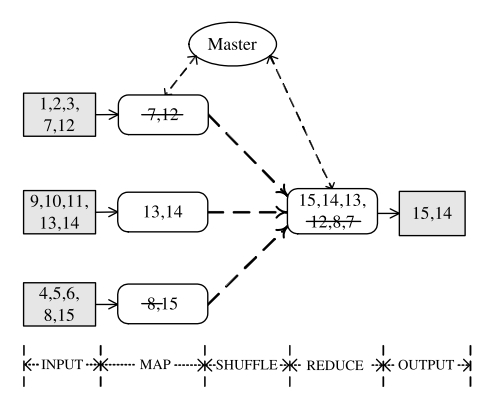
\includegraphics[width=.5\linewidth]{7_18_commapreduce.png}\\
  \caption{Example of top-$k$ query}\label{fig:commapreduce}
\end{figure}


The basic idea of ComMapReduce is to obtain a global \emph{shared information} to filter unpromising data, and thus reduce the communication cost in the shuffle phase. Suppose that now the example query in Figure \ref{fig:commapreduce} is processed by the ComMapReduce method. After the second Mapper produces its local result (13, 14), it shares the minimal result 13 with other Mappers. When the first Mapper receives the information, it realizes that its local data is not useful for obtaining the final result, so it will not send them to the Reducer in the shuffle step and the communication cost is reduced.

In the ComMapReduce framework three communication strategies can be applied, namely Lazy, Eager and Hybrid. They differ in when the Mappers received the shared information. In the Lazy strategy, after each Mapper produces its local result and send it to the coordinator, it waits for all the other Mappers until the coordinator receives all the local results. Then the global shared information will be distributed to all Mappers, according to which they locally prune the outputs. In the Lazy strategy, after each Mapper completes, it sends its local output to the coordinator and receives a global shared information simultaneously. The coordinator also sends the shared information to all Mappers that already completed. In the hybrid strategy, a Mapper sends its local output at once when it completes, but the coordinator waits for a period time to receive the other Mappers' messages before sending the global shared information.

The paper further develops two optimization strategies to enhance the performance of ComMapReduce, namely \emph{Prepositive Optimization Strategy (PreOS)} and \emph{Postpositive Optimization Strategy (PostOS)}. In PreOS Mappers can retrieve shared information in their initial phase and use it to prune their local data. In PostOS after the intermediate data is sent to the Reducers, the Reducers retrieve global shared information from the coordinator and filter their input data again.

The experimental section takes four query processing applications, top-$k$, $k$NN, skyline and join, as examples to evaluate the performance of ComMapReduce. The experimental results demonstrate that the performance of ComMapReduce is superior to MapReduce in all metrics (running time, number of reduced input records and filter percentage).

\section{RankTopic: Ranking Based Topic Modeling \cite{DLLZW12}}

This paper investigates how to utilize the importance of documents to improve \emph{topic modeling}, and proposes a method called \emph{RankTopic} which incorporates link based ranking into topic modeling.

Topic modeling aims to represent documents as a distribution over topics instead of words, with the benefit that topics are usually of much lower dimensions and are much more interpretable than words. However, most existing approaches do not consider the importance of the documents, which motives the RankTopic method proposed in this paper.

\begin{figure}[h]
  \centering
  % Requires \usepackage{graphicx}
  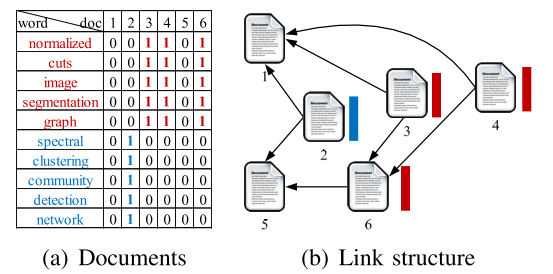
\includegraphics[width=.5\linewidth]{7_18_doc.png}\\
  \caption{Example of artificial documents and network}\label{fig:docnet}
\end{figure}

\begin{figure}[h]
  \centering
  % Requires \usepackage{graphicx}
  \includegraphics[width=.5\linewidth]{7_18_topic.png}\\
  \caption{Example of artificial documents and network}\label{fig:topic}
\end{figure}

For example Figure \ref{fig:docnet} presents a set of artificial documents and a document network. There are two topics in these documents, which are colored by red and blue respectively. Higher bars indicate more proportions of the labeled topics. Figure \ref{fig:topic} shows the topic output of the \emph{iTopic} \cite{SHGY09} method and the proposed RankTopic method. iTopic treats neighboring documents as equally important. However we can observe that document 6 should be of better importance, because it is cited by other two documents. RankTopic takes this into account, and document 5 is assigned with more red topic propotions.

The basic idea of RankTopic is to incorporate the \emph{topical pagerank} \cite{NDQ06} method into the classic topic modeling algorithm \emph{PLSA} \cite{Hofmann99}. Next I will briefly explain the two underlying algorithms respectively.

Topical pagerank produces a ranking vector for each document, in which each element represents the importance score of the document on each topic. Let $\gamma_{zi}$ denote the ranking of document $i$ on topic $z$, $\gamma{.j} = \sum_{z=1}^K \gamma_{zj}$ denote the global ranking of document $j$, $\theta_{jz}$ be the topic proportion of document $j$ on topic $z$ and $I_i$ is the set of in-link neighbors of documents $i$. Topical page rank is formally expressed as
$$\gamma_{zi}^{(t)} = \lambda \sum_{j \in I_i} \frac{\alpha \gamma_{zj}^{(t-1)} + (1-\alpha)\theta_{jz}\gamma_{.j}^{(t-1)}}{|O_j|} + (1-\lambda) \frac{\theta_{iz}}{M}.$$
The final topical rank result $\gamma_{zi}$ is iteratively computed from a randomly initialized value.

Given a collection of $M$ documents $D$, let $V$ denote the size of the vocabulary and $K$ be the number of topics. PLSA aims to maximize the likelihood of $D$ with respect to parameters $\Theta$ and $B$:
$$P(D|\Theta,B) = \prod^M_{i=1} \prod^V_{w=1} (\sum_{z=1}^K \theta_{iz} \beta_{zw})^{s_{iw}}.$$
Intuitively, this is a generating model meaning that document $i$ is of topic $z$ with probability $\theta_{iz}$ and topic $z$ generates word $w$ with probability $\beta_{zw}$.

In the proposed RankTopic model, the likelihood of a collection of documents $D$ is defined as
$$P(D|\gamma, \pi, \phi, \beta) = \prod^M_{i=1} \prod^V_{w=1} (\sum_{z=1}^K [\xi \gamma_{zi} + (1-\xi)\phi_{zi}]\pi_z \beta_{zw})^s_{iw}.$$
Then the maximum likelihood estimation is adopted to derive the model parameters. Since $\phi_{zi}$ in the formula is considered as hidden variables, the local maximum of the likelihood is obtained by a \emph{expectation maximization (EM)} based algorithm.

The experimental section compares the RankTopic model with some state-of-the-art topic models, namely PLSA, LDA, iTopic and \emph{Relational Topic Model (RTM)} \cite{CB13}, in terms of perplexity, document clustering and classification accuracy, and topic interpretability. It is shown that with proper balancing parameter $\xi$ RankTopic performs consistently better than PLSA, LDA and iTopic, and is comparable with RTM in all the aspects.


\section{Location Selection for Utility Maximization with Capacity
Constraints \cite{SHCZD12}}

This paper proposes a new type of query called \emph{location selection query for utility maximization}. After applying three pruning rules to a baseline solution, it obtains an efficient algorithm to answer the query.

\begin{figure}[h]
  \centering
  % Requires \usepackage{graphicx}
  \includegraphics[width=.4\linewidth]{9_12_CIKM1.png}\\
  \caption{Query example}\label{fig:CIKM1}
\end{figure}

With the assumptions that a client seeks services from his nearest facility, and a facility provides service to clients in the order of their proximity, the proposed query selects all possible locations such that setting up a new facility at these locations will maximize the number of served clients. For example in Figure \ref{fig:CIKM1}, the capacities of distribution centers $f_1, f_2$ and $f_3$ are 3,4 and 5 respectively. Circles and black dots indicate the served and unserved customers. The customer $c_4$ is unserved since its nearest center $f_1$ only has a capacity of 3, which has been used up by $c_1, c_2, c_3$ since they are nearer to $f_1$ than $c_4$. If a new center with a capacity of 4 is to be built, setting it up in any region of $\{R_1, R_2, R_3, R_4, R_5\}$ will server 4 more customer, which reaches its full capacity. Therefore, $\{R_1, R_2, R_3, R_4, R_5\}$ is the answer to this query.

The algorithm proposed in this paper makes use of the concept of the \emph{nearest facility circle (NFC)}. Given a client $c$, the NFC of $c$ (denoted as $n(c)$), is a circle that centers at $c$ with radius as the distance between $c$ and its nearest facility. The paper denotes the set of all the points within $n(c)$ as $\bar{c}$ and the set of all the points outside as $\hat{c}$.

\begin{figure}[h]
  \centering
  % Requires \usepackage{graphicx}
  \includegraphics[width=\linewidth]{9_12_CIKM2.png}\\
  \caption{Arc NFC relationship and different examples}\label{fig:CIKM2}
\end{figure}

The basic idea is that the answer to the proposed query consists of several maximal regions, where each maximal region is enclosed by arcs generated from some NFCs intersecting with each other. For example Figure \ref{fig:CIKM2} (b) shows an example of four maximal regions $\bar{c_1} \cap \bar{c_2}, ..., \hat{c_1} \cap \hat{c_2}$. Note that a maximal region does not have to be a connected region, as shown in Figure \ref{fig:CIKM2} (c). It is possible to describe all maximal regions by enumerating $\bar{c}$ and $\hat{c}$. However, some enumeration may have no corresponding maximal regions. For example, in Figure \ref{fig:CIKM2} (c), the region $\hat{c_1}\bar{c_2}\bar{c_3}$ actually does not exist. So the next step of the paper is to propose a technique to check the validation of an enumeration.

The paper adopts an incremental way of checking. During the validating process, a temporary maximal region $R$ is incrementally maintained. When checking a new client, it needs to update the arcs enclosing $R$. Given an NFC, a point has three states in terms of their positional relationship: in, on, and out. There are 12 cases of the relationship, which are shown in Figure \ref{fig:CIKM2} (a). Figure \ref{fig:CIKM2} (b)(c) show an example of the validating process. In this example, it needs to validate $\bar{c_1}\hat{c_2}\hat{c_3}$. Let the temporary maximal region be $R=\bar{c_1}\hat{c_2}$, whose enclosing arcs are $a_1$ and $a_2$. When checking $c_3$, both $a_1$ and $a_2$ are updated, leading to 4 smaller arcs.

The baseline algorithm proposed in the paper is to enumerate all combinations of clients, validate each enumeration, compute the increment of utility and get the result. An example is shown in \ref{fig:CIKM2} (d). There are six NFCs, and each is assigned with an unique ID. It starts from the NFC with the smallest ID 1. Since 1 only intersects 2 and 3, the regions that need to be enumerated are $123\hat{4}\hat{5}\hat{6}$, $12\hat{3}\hat{4}\hat{5}\hat{6}$, $1\hat{2}3\hat{4}\hat{5}\hat{6}$, and $1\hat{2}\hat{3}\hat{4}\hat{5}\hat{6}$. The other NFCs are then enumerated in a similar way.

The paper further proposes three pruning rules to speedup the search process: 1) In the baseline algorithm, the maximal regions are found by enumerating each NFC $n(c)$ and other clients that intersect it with larger IDs. In the first technique, before enumerating $n(c)$ it estimates the upper bound utility of all maximal regions within $n(c)$, which helps to determine whether $n(c)$ is worth exploring or not. 2) In the second technique, when enumerating related clients for $n(c)$, it uses the maximal workload that a facility can be shared as an upper bound. 3) During the enumeration of $n(c)$ and its related clients, if the temporary maximal region corresponds to a non-exist region, there is no need to enumerate remained clients.

In the experimental study, the paper evaluates the performance of the proposed method in terms of CPU time while varying different parameters. It is shown that when all the pruning techniques are applied, the algorithm outperforms the baseline by up to three orders of magnitude.

\section{Top-k Most Incremental Location Selection with Capacity Constraint \cite{SHCDZ12}}

This paper studies a new type of \emph{bichromatic reverse nearest neighbor (BRNN)} based query, which aims at finding most promising candidate locations to increase the overall service quality. It proposes an $O(n \log n)$ algorithm and conducts extensive experiments on it.

In a BRNN query the location points are separated into two sets $W$ and $R$. Given a location $w \in W$, a BRNN query returns all $r \in R$ whose nearest neighbor is $w$. In the new proposed problem in this paper, each facility point $w \in W$ is associated with a \emph{capacity} $c(w)$, and each customer location $r \in R$ is associated with a \emph{weight} $wt(r)$. If $w$ is responsible to serve its reverse nearest neighbor $r$, the capacity $c(w)$ will be consumed by the weight $wt(r)$ (a customer location can be partially served). The paper  assumes that each $w$ serves its customers in decreasing order with respect to the Euclidean distance, until its capacity is fully occupied.

\begin{figure}[h]
  \centering
  \subfigure[Before $p_1$ is added]{
    \label{fig:topka} %% label for first subfigure
    \includegraphics[width=1.4in]{7_18_topk1.png}}
  \subfigure[After $p_1$ is added]{
    \label{fig:topkb} %% label for second subfigure
    \includegraphics[width=1.4in]{7_18_topk2.png}}
  \caption{Example of BRNN query with capacity constraint}\label{fig:topk}
\end{figure}

For example in Figure \ref{fig:topk}, circles, small and big rectangles denote customer locations ($R$), facilities ($W$) and BRNN sets respectively, and the numbers beside each $r$ denote the serving order. The black circles in Figure \ref{fig:topka} denote the customers that are not fully served due to capacity restriction. In Figure \ref{fig:topkb} if a new facility $p_1$ is established, the workload will be shared and more weight will be served. The problem proposed in this paper, is to find the top-$k$ locations from a given set $P$ that cause maximal increments to the total served weight.

The first step is to reduce the query to a simpler form. A customer location is said to be $\epsilon$-served, if $\epsilon \cdot wt(r)$ of the weight is served. Given a set of existing facilities $W$, the service quality is defined as $sq(W) = \sum_{r\in R} \epsilon(r) wt(r)$. If a new facility $p$ is established, the service quality will be increased by $inc(c) = sq(W \cup \{p\}) - sq(W)$. So finding $k$ most promising candidates is equivalent to find the top-$k$ $p \in P$ with maximal $inc(p)$.

The basic idea of the proposed algorithm is that each candidate location can only influence the customers near to it, so lots of far away customer locations can be pruned during the computation of $inc(p)$. The proposed method exploits the concept of \emph{nearest facility circle (NFC)}, which is a circle denoted by $nfc(r,w)$ that centers at $r$ and has a radius of $dist(r,w)$. If $p$ falls into $nfc(r,w)$, then $p$ will influence the customer $r$ if it is established. The algorithm maintains several spatial indices for processing necessary NN and RNN queries, which are used to compute the influenced customers for a given $p$ efficiently.

The experimental section compares the proposed method with a naive solution. It is shown that the proposed method outperforms the naive method by nearly 4 orders of magnitude in terms of CPU time. Even only using the pruning techniques (without using spatial indices), the improvement is about 2 orders of magnitude.

\section{DuoWave: Mitigating the curse of dimensionality for uncertain data \cite{MZLC12}}

The paper addresses the problem of the \emph{curse of dimensionality} for uncertain data. It proposes an indexing technique called \emph{DuoWave} for uncertain objects. It shows that DuoWave can efficiently support \emph{probabilistic range queries} and \emph{similarity queries}, based on a filter-and-refine paradigm.

An \emph{uncertain object} $X$ in the $d$-dimensional data space is represented by an uncertain region $X.ur = \{[X.l_1, X.u_1],..., [X.l_d, X.u_d]\}$. Each object $X$ is also modeled by a \emph{probability density function (pdf)} $X.pdf$ to represent its probability distribution.

The paper focus on two types of queries: the \emph{Threshold Probabilistic Range (TPR) query} and the \emph{Threshold Probabilistic $\epsilon$-similarity (TPS) query}. Given a set of uncertain objects $DB$ and a query rectangle $R_Q$, TPR retrieves all uncertain objects in $DB$ whose probability of residing in $R_Q$ is greater than a threshold. In TPS queries the similarity of two uncertain objects $X$ and $Q$ is measured as
$$\int_{X.ur}(\int_{Q.ur} \delta(x,q)\cdot Q.pdf(q) dq) \cdot X.pdf(x) dx,$$
where $\delta(x,q)$ is 1 if $|q-x| \leq \epsilon$ or 0 otherwise. Given a set of uncertain objects $DB$ and an uncertain query $Q$, TPS retrieves all $X \in DB$ such that the similarity between $X$ and $Q$ is less than a predefined threshold. Next we will see how these two types of queries can be efficiently processed by the DuoWave index.

The DuoWave index is a compression of the original data file. The compression consists of three steps: 1) approximating uncertain objects' probability distributions using \emph{histograms}; 2) performing \emph{wavelet transform} on the histograms; 3) selecting only some dimensions to be kept in the DuoWave index.

Figure \ref{fig:duowave_index} shows an example of the DuoWave index. Given an uncertain object $X$ in a 2-dimensional space, the method will first construct histograms for each dimension (this step is not shown in the figure). Then it will use the wavelet transformation to compress the histograms in each dimension. In this example, the histograms in the 1st dimension are compressed as the sequence $\{-0.045, -0.02, ..., 0.06\}$ (shown as the \emph{abridged wavelet coefficients}), along with the \emph{coe-bitmap} indicating which coefficients are omitted. Finally, the method decides that the 2nd dimension is not important enough to be retained, and this is represented by the \emph{dim-bitmap} 10.

\begin{figure}[h]
  \centering
  % Requires \usepackage{graphicx}
  \includegraphics[width=.9\linewidth]{7_11_duowave.png}\\
  \caption{Index entry of an uncertain object}\label{fig:duowave_index}
\end{figure}

A TPR query is processed with the DuoWave index as follows. In the filter phase, the DuoWave index entries are scanned one by one. If $X.ur$ does not intersect the query region, $X$ must not be an answer and we can safely discard it. Otherwise the information in the index is used to derive an upper bound of the probability of $X$ being within the query region. If the upper bound is less than the threshold, the corresponding object $X$ will be discarded. Then in the refine phase, the remaining candidate objects will be check by exact computation to decide which ones are in the real answer set. The difficulty of this scheme is to derive an upper bound as tight as possible from the information in the index entry. The paper develops sophisticated mathematics to solve this problem, and the details are omitted here. The basic idea of processing TPS queries is also similar.

The experimental section performs comparative studies on pruning power, total query response time and I/O cost with the \emph{U-tree} \cite{TCXNKP05} and \emph{APLA} \cite{LS07} methods. It is shown that the DuoWave index consistently outperforms the other alternative approaches. In some cases the improvement over APLA are 4 times, 3 times and up to 10 times in terms of pruning power, response time and I/O cost respectively. The improvement over U-tree is over 10 times in all metrics.

\section{Boosting Moving Object Indexing through Velocity Partitioning \cite{NHZW12}}

This paper proposes the \emph{velocity partitioning (VP)} technique, which exploits the skew in velocity distribution to speed up query processing using moving object indexes.

\begin{figure}[h]
  \centering
  % Requires \usepackage{graphicx}
  \includegraphics[width=.7\linewidth]{7_11_obj.png}\\
  \caption{Objets indexed by an unpartitioned and partitioned indexes}\label{fig:VP_obj}
\end{figure}

\begin{figure}[h]
  \centering
  % Requires \usepackage{graphicx}
  \includegraphics[width=.7\linewidth]{7_11_exp.png}\\
  \caption{Expansion of search space}\label{fig:VP_exp}
\end{figure}

In many data structures that index moving objects, such as \emph{TPR-tree} \cite{SJLL00}, \emph{B$^x$-tree} \cite{JLO04} and their variants, the search region need to be extended if the query is for the future. The VP technique exploits the fact that velocity partitioning can reduce search space expansion. For example Figure \ref{fig:VP_obj} presents some moving objects that are maintained by an unpartioned or two partitioned indexes respectively, and Figure \ref{fig:VP_exp} presents the search spaces and their expansions on the corresponding indexes. In Figure \ref{fig:VP_exp} (a), if the objects are indexed by the unpartitioned index, the search range for a future query need to be expanded to four directions. In contrast, if the objects are indexed by two partioned structures, the total search space expansion is greatly reduced.

The system of the VP technique has two main components, a \emph{velocity analyzer} and an \emph{index manger}.

The velocity analyzer partitions the velocities of objects in order to find the \emph{dominant velocity axes (DVAs)}. This technique is a combination of \emph{principal components analysis (PCA)} and \emph{$k$-means clustering}. In classic $k$-means clustering, each data object is assigned to its closest centroid where the distance is measured by the Euclidean metrics. In the VP technique, the distance is computed in two steps: 1) for each candidate cluster, it computes the \emph{principle components (PC)} of the objects in the cluster; 2) the distance of a object to a cluster is calculated as the perpendicular distance to the 1st PC of the cluster. Finally the velocity analyzer produces $k$ DVAs, where $k$ is a user defined parameter.

The index manager maintains an index tree for each DVA. When an object need to be inserted, the index manager first finds the DVA index $i_{min}$ whose perpendicular distance from the object is the smallest. Then the manage inserts the object to the index $i_{min}$. Here the underlying index structure ($i_{min}$) can be a TPR-tree, a B$^x$-tree or their variants. Other operations like deletion and update are also similarly performed. Given a moving range query, the index manager needs to query each of the indexes separately and merge the results. The proposed method also supports other query types, namelly the time slice range query, time interval range query, and they can be similarly processed.

The experimental section compares the performance of the VP technique applied to the B$^x$-tree and the TPR$^*$-tree against their unpartitioned  counterparts. It is shown that the index structures equipped with the VP technique outperform their original versions consistently in terms of query I/O and query execution time. In some cases the B$^x$(VP)-tree outperforms its counterpart by up to 3.4 times for query I/O and up to 2.8 times for execution time.

\section{Probabilistic Voronoi Diagrams for Probabilistic Moving Nearest Neighbor Queries \cite{ATZR12}}

This paper proposes the \emph{probabilistic Voronoi diagram (PVD)} for processing the \emph{probabilistic moving nearest neighbor (PMNN) queries}. The authors provide two techniques: a pre-computation approach and an incremental approach.

In a $d$-dimensional  space, an \emph{uncertain object} is represented by a $d$-dimensional uncertain range $R$ and a \emph{probability density function (pdf)} representing the distribution of the object. Intuitively it means that the object's accurate location is within $R$. A \emph{probabilistic nearest neighbor (PNN) query} is defined as follows: Given a set $O$ of uncertain objects in a $d$-dimensional database, and a query point $q$, a PNN query returns a set $P$ of tuples $(o_i, p_i)$, where $o_i \in O$ and $p_i$ is the probability that $o_i$ is the nearest object to the query point. In a PMNN query, the query point is continuously moving.

\begin{figure}[h]
  \centering
  % Requires \usepackage{graphicx}
  \includegraphics[width=.5\linewidth]{7_11_pnn_example.png}\\
  \caption{Example of PNN query}\label{fig:PNN_example}
\end{figure}

In the example presented in Figure \ref{fig:PNN_example} there are three uncertain objects ($o_1, ... o_3$) around the query point $q$. Each of the three objects can be a nearest object of $q$, so the PNN query returns $P = \{(o_1,p_1),(o_2,p_2),(o_3,p_3)\}$, where $p_i$ is the probability that $o_i$ is indeed the nearest object to $q$. The computation of $p_i$ involves integration and the details are omitted here.

Given a set of uncertain objects $o_1,..., o_n$, the basic idea of PVD is to partition the data space into a set of \emph{probabilistic Voronoi cells (PVCs)}. Each cell $PVC(o_i)$ is a region is the data space, where each data point is most probably being the nearest neighbor to $o_i$.

It should be mentioned that the proposed PMNN query and PVD can be applied to uncertain objects with any distribution. By the following proposed algorithms only applies to objects with uniform distribution.

The paper develops algorithms for computing PVDs in 1d and 2d data space respectively. Computing PVDs is equivalent to computing the probabilistic bisectors $pb_{o_io_j}$ for every two adjacent objects $o_i$ and $o_j$. In 1d data space $pb_{o_io_j}$ is a point $x$, such that $o_i$ and $o_j$ have the same probability being the nearest neighbor to $x$. Similarly, $pb_{o_io_j}$ in 2d data space is a line, such that $o_i$ and $o_j$ have the same probability being the nearest neighbor to every point in the line.

The computation of PVDs in 1d data space is analysis in a case based manner. An uncertain object in 1d data space is represented by a 1d range. The paper proves that if two objects $o_i$ and $o_j$ have equal length, or $o_i$ and $o_j$ are non-overlapping and there is no other object between them, then $pb_{o_io_j}$ is the bisector of the midpoint of the two ranges. For other cases, the algorithm will first initialize the candidate bisector without considering other objects, and then performs a step-wise search until a bisector is found.

The exploration in 2d data space follows a similar case base discussion. The paper first discusses some special cases where the bisectors can be accurately computed. For other cases, the algorithm will initialize the bisectors by reducing the problem to the special cases, and then perform a step-wise search to find the exact bisectors.

PVD can also be incrementally computed. The basic idea is to retrieve a set of surrounding objects for the given query point, then create a PVD based on the retrieved objects. When current retrieved objects are not enough to guarantee one of the known object is the nearest, the algorithm requests more objects incrementally and repeats the process. The algorithm variants with and without incremental technique are denoted as \emph{P-PVD-PMNN} and \emph{I-PVD-PMNN} respectively.

The experimental section compares P-PVD-PMNN and I-PVD-PMNN with a naive approach (Naive-PMNN), which processes a PMNN query as a sequence of static PNN queries. It is shown that P-PVD-PMNN outperforms  Naive-OMNN by at least an order of magnitude in all evaluation metrics (response time, I/O cost and communication cost). I-PVD-PMNN is on average about 10 times faster than Naive-PMNN in response time, and is better by 2-3 orders of magnitude for I/O and communication cost.

\section{An Adaptive Algorithm for Online Time Series Segmentation with Error Bound Guarantee \cite{XZRP12}}

This paper proposes a method to approximate time series by a set of candidate functions (polynomials of different orders, exponential functions, etc.), and adaptively choose the most compact one online as the pattern of the time series changes. The approximation guarantees that each data point in the resulted series has an absolute error less than a predefined error bound $\delta$.

The basic idea is to use of \emph{segmentation}, which is also applied in the \emph{Piecewise Linear Approximation (PLA)} method developed in \cite{GS01} and the \emph{Feasible Space Window (FSW)} method. PLA divides a time series into segments and uses a linear function to approximate each segment. The work of FSW develops the concept called \emph{Feasible Space (FS)}, which is also used in this paper. Intuitively, given an absolute error bound $\delta$, FS is an area in the data value space such that any straight line in the area is a candidate approximation. For example in Figure \ref{fig:fsw_example}, $P_0, P_1 $ and $P_2$ are the first three points in the data series. $P_1^\top = P_1.y + \delta$ and $P_1^\bot = P_1.y - \delta$ are used to compute the bounds $u_1$ and $l_1$ of the FS. Each line in the region formed by $u_1$ and $l_1$ is a possible approximation for the first two points. When a new point $P_2$ is introduced, the method will compute the FS of $P_0$ and $P_2$, and then intersect the new FS with the previous one to get the dark-shaded region.

\begin{figure}[h]
  \centering
  % Requires \usepackage{graphicx}
  \includegraphics[width=.5\linewidth]{7_11_fsw_example.png}\\
  \caption{Example of FSW}\label{fig:fsw_example}
\end{figure}


The \emph{Adaptive Approximation (AA)} algorithm proposed in this paper is more general than FSW, since the approximation functions can be polynomials of differen orders and exponential. The basic idea of AA is to build feasible space like the FSW method, but the feasible values are for the functions' coefficients. For example we want to approximate two data points $p_0(x_0, y_0)$ and $p_1(x_1, y_1)$ with the second-order polynomial function $y = ax^2 + bx + c$, we can derive that the coefficients $a$ and $b$ must satisfy the following inequalities:
$$y_0 + a(x_1^2-x_0^2) + b(x_1-x_0) \leq y_1 + \delta;$$
$$y_0 + a(x_1^2-x_0^2) + b(x_1-x_0) \leq y_1 - \delta.$$
The coefficient values of $a$ and $b$ are restricted by bounds $l_1$ and $u_1$ as Figure \ref{fig:space} shows. When new data arrives, the algorithm will compute new bounds and intersect the FS with the previous result, which is similar to the process of FSW. If the FS is empty after $p_n$ is added, then the algorithm segments the series at $p_{n-1}$, and then initializes $p_{n-1}$ and $p_n$ as the first two points of the next new segment.

\begin{figure}[h]
  \centering
  % Requires \usepackage{graphicx}
  \includegraphics[width=.5\linewidth]{7_11_space.png}\\
  \caption{Feasible coefficient space for quadratic functions}\label{fig:space}
\end{figure}

The experimental study compares the proposed AA algorithm with the FSW algorithm, and the performance is measure by the \emph{Number of Approximated Points per Parameter (NAPP)} and average approximation error, where NAPP indicates the compactness of the approximation. It is shown that AA outperforms FSW consistently in terms of NAPP. In some cases the improvement factor is up to 2 times. In some cases, AA also results in much lower errors (decrease up to 50\%) than those caused by the FSW algorithm.

\section{The Min-dist Location Selection Query \cite{QZKLX12}}

This paper formulates a new type of location optimization problem called the \emph{min-dist location selection query}, and proposes three algorithms for processing it. The paper also provides a detailed comparative cost analysis on the various algorithms and conducts comprehensive experiments over them.

Given a set of clients $C$, a set of existing facilities $F$ and a set of potential locations $P$, a min-dist location selection query is to find the location in $P$ that can minimize the average distance between a client and her nearest facility, so that people can access the facilities in the shortest time.

\begin{figure}[h]
  \centering
  % Requires \usepackage{graphicx}
  \includegraphics[width=.6\linewidth]{7_11_mindist.png}\\
  \caption{Example of min-dist location selection query}\label{fig:mindist}
\end{figure}


For example in Figure \ref{fig:mindist}, if a new facility is to be built at $p_2$, it will results in a smaller average distance between a client and her nearest facility. The gain of building the new facility at $p_2$ is larger than building at $p_1$, so in this example $p_2$ will be selected as the answer of the query.

The first observation of the paper is that the min-dist query can be reduced to a simpler form. We call the distance between a client and her nearest facility the \emph{nearest facility distance (NFD)}. Given a location $o$, the \emph{influence set} of $o$ (denoted as $IS(o)$) is the set of clients that can get NFD reduction if a new facility is built there. The min-dist query is to minimize the sum of all clients' NFD. If a new facility $p$ is established, the sum of all clients' NFD will decrease, and we call it the \emph{distance reduction} of $p$ and denote it as $dr(p)$. So the min-dist query is equivalent to finding a potential facility $p$ with maximal $dr(p)$.

The first proposed method is called the \emph{quasi-Voronoi cell (QVC)} method. A QVC is a region that encloses the actual Voronoi cell, and it can be used as a good approximation. For each potential location $p$, the algorithm forms its QVC, so that any customer outside the QVC cannot be influenced by $p$. In this way, the influence set $IS(p)$ can be efficiently computed.

The second method exploits the concept of \emph{nearest facility circle (NFC)}, so the paper calls it the NFC method. Since for a potential location $p$, $c \in IS(p)$ if and only if $p$ is inside $NFC(c)$, the NFC technique can also efficiently prune those customers that cannot be influenced. However, in order to decide if a location is inside an NFC, the method need to maintain an extra index structure.

Since both QVC and NFC have their advantages and drawbacks, the paper further develops the \emph{maximum NFC distance (MND)} method. MND is based on NFC as its name suggests. However unlike the NFC method where extra index structures are necessary for maintaining the NFCs of all clients in a node, the MND method uses just one value to describe a region that encloses the NFCs of all clients. The value is a tight bound that encloses the NFCs of all clients in a node, and the paper call it the maximum NFC distance. Sophisticated mathematics is developed for the efficient computation of the maximum NFC distance, and the details are omitted here.

In the experimental study, the paper compares the proposed QVC, NFC and MND algorithms with a naive \emph{sequential scan (SS)} approach, in terms of running time, I/O cost and index size. It is shown that MND and NFC are the most efficient methods for running time and I/O cost (with improvement over an order of magnitude in some cases). The MND method has close efficiency to NFC without the need of maintaining an additional index (for the 100K datasets, the index size if MND drops to about 60\% of that of the NFC method).

\section{A highly optimized algorithm for continuous intersection join queries over moving objects \cite{ZQLWW12}}

This article is an extended version of a previous paper \cite{ZLRB08}. The goal of the study is to propose a method to efficiently process continuous intersection join queries over moving objects with nonzero extents, which monitors two sets of moving objects and reports every pair of intersecting objects.

Recall that the previous paper introduces two naive approach, and then proposes the \emph{time-constrained (TC)} processing method.

The first naive approach, called \emph{NaiveJoin}, works as follows. Each dataset $A$ and $B$ is indexed by a \emph{TPR-tree} $tr_A$ and $tr_B$ respectively. The basic idea is to use the bounding relationship to prune the search. Specifically, if node $N_A$ does not intersect node $N_B$, then none of the entries in their subtrees will intersect each other. In this way, lots of unnecessary search can be pruned.

The second naive approach, called \emph{extending time-parameterized join algorithm (ETP-Join)}, is based on a previous paper \cite{TP02} that introduces the \emph{time-parameterized (TP) intersection queries}. The original TP join query does not answer the continuous join query directly, but it can be extended to serve the purpose.

The previous paper observes that ETP-Join has to run TP-Join frequently, so its problem is computing the result for too short a time interval in each run. On the other hand, the problem of NaiveJoin is computing the result for too long a time interval. Based on this observation, the previous paper proposed the TC algorithm, which tries to achieve a balance by imposing a time constraint over the query processing. The efficiency is further optimized by grouping objects into buckets to tighten the time constraint. A set of techniques on static intersections join are also applied, such as the \emph{plane sweep} and \emph{intersection check}.

The new contributions of this journal version are as follows: 1) It presents a few new techniques to reduce the I/O cost of the algorithms. 2) More importantly, it models the cost of the algorithm, with which the optimal value for the maximum update interval can be found. 3) It conducts additional experiments to show the effectiveness of the new techniques, and the accuracy of the cost model.

The first technique is the improved node accessing order in intersection check. The basic idea is that even if node $N_A$ intersects $N_B$, it is still possible that no entry of $N_A$ intersects any entry of $N_B$. So when joining two intersecting nodes, the proposed technique always access first the one which is most recently accessed. Since this node is most recently accessed, its probability of still being in buffer is high. Thus, it can perform intersection check on it without additional I/O cost.

The second technique is group processing of updates. The motivation is to reduce the number of tree traversals and hence improve node access performance. At every timestamp, it groups all updated objects of a dataset and join it with the other joining tree.

In the previous discussion, it is assumed that the maximum update interval, $T_M$, is a given parameter. The paper examines the problem of finding an optimal $T_M$ value by establishing an accurate cost model. It shows that the average cost for processing all the updated objects in $tr_A$ per timestamp is
$$C_A = (n_A p_v + \frac{n_A (1 - p^v)^{T_M}}{T_M}) f_A,$$
where $n_A$ is the number of objects in $tr_A$, $f_A$ is the average cost of update, and $p_v$ is the probability of a voluntary update. The average cost in $tr_B$ can be similarly computed. Finally, the optimal $T_M$ can be decided according to the cost model.

In the experimental section, the new results show the effectiveness of the new techniques and the accuracy of the cost model. For example if the test system runs with a randomly chosen $T_M$ value, the average number of node accesses per timestamp is about 54\% larger than that of running the system with the optimal $T_M$ value.

\section{Continuous Detour Queries in Spatial Networks \cite{NTSZR12}}

This paper proposes the \emph{continuous detour query (CDQ)}, which aims to find the shortest route between two locations with a stopover. It develops a method called the \emph{incremental order $k$ shortest path tree (I$k$SPT)} algorithm that finds the first $k$ \emph{minimum detour objects (MDOs)}. Here a MDO is a stopover that minimizes the sum distances from the start to the stopover, and from the stopover to the destination.

An example scenario of CDQ is that Alice is on her way to Bob's house, and she searches for a nearby take-away restaurant to buy a pizza. Here we want to find the shortest path between Alice's location and Bob's house, with the constraint that a restaurant (MDO) is on the trajectory. The query is continuous, in the sense that Alice's location keeps changing (but the destination is fixed in the proposed problem).

The basic idea of I$k$SPT is similar to that of the classic \emph{Dijkstra's algorithm}. In Dijkstra's algorithm, we can build a \emph{shortest path tree (SPT)} based on the greedy strategy, and then find the shortest path of a query node by traversal back to the root (which represents the destination location). In the I$k$SPT algorithm, the root node is the query destination (Bob's house in the running example), and the nodes in depth 1 represent all the detour objects. The distances between the detour objects and the root are the lengths of their shortest paths in the graph. Another difference is that in the order-$k$ tree each node appears for $k$ times.

\begin{figure}
  \centering
  % Requires \usepackage{graphicx}
  \includegraphics[width=.6\linewidth]{74_spt.png}\\
  \caption{Order-$k$ SPT with $k$ of 2}\label{fig:spt}
\end{figure}


Figure \ref{fig:spt} is an example of an order-2 SPT. As aforementioned $q_e$ is the destination (Bob's house). If Alice's location is now at $n_2$, we can see that the two shortest paths are $q_e$-$a$-$n_7$-$n_4$-$n_2$ and $q_e$-$d$-$n_2$. Once the $k$-SPT is built, the first $k$ MDOs can be continuously computed without much cost.

The paper further develops a method that can incrementally construct the $k$-SPT. The idea is based on the observation that if the start point is given in the query, it is unnecessary to build the whole $k$-SPT since the faraway nodes are irrelevant, and this results in the final I$k$SPT algorithm. Specifically the algorithm sorts the MDOs by their distances, and in each loop only the nodes with distances no larger than the current MDO will be processed.

The experimental section compares the I$k$SPT method with two other alternative approaches: the \emph{$k$SPT method} and the \emph{incremental network expansion (INE)} method. Here $k$SPT is the version of the proposed method without applying the incremental technique, and INE is adapted from the paper \cite{PZMT03}. It is reported that I$k$SPT is 3.1 times as fast as INE and 2.3 times as fast as $k$SPT in response time. In terms of the traversal cost, I$k$SPT has an improvement factor of 2.3 times and 2.4 times in comparison to INE and $k$SPT respectively.



\section{A Moving Object Index for Efficient Query Processing with Peer-Wise Location Privacy \cite{LJZLJ11}}

This paper proposes an indexing method that can efficiently support range and $k$ nearest neighbor queries, while preserving \emph{peer-wise location privacy}. It also discusses the I/O cost model of the proposed data structure, and shows its accuracy with experiments.

Protecting peer-wise privacy is to protect a user's location from unauthorized peer users. In this paper, a user can specify his privacy requirement by the \emph{Location-Privacy Policies (LPP)}. LPP assigned by user $u_1$ to $u_2$ is denoted as $P_{1 \rightarrow 2} = \langle role, loc_r, t_{int} \rangle$, which means that if $u_2$ is related to $u_1$ by relationship $role$, then $u_2$ is allowed to see $u_1$'s location when $u_1$ is located in $loc_r$ during $t_{int}$. For example, Bob lets his colleagues see his location when he is in town during work hours. The corresponding LLP is $P = \langle colleague, Chicago, [8 a.m., 5 p.m.] \rangle$.

This paper proposes a data structure called the\emph{ Policy-Embedded B$^x$-tree (PEB-tree)}, which can efficiently answer two types of privacy-aware queries: the \emph{privacy-aware range query (PRQ)} and the \emph{privacy-aware $k$ nearest neighbor (P$k$NN) query}. PRQ returns a set of users that fall within the query range, and these users allow themselves to be seen by the query issuer. Similarly P$k$NN returns $k$ nearest users that allow themselves to be seen. For example in Figure \ref{fig:PEB_example}, the query issuer is $u_1$ and his friends are represented by the star symbols (the white circles represent other users). Suppose that according to the privacy policies, only $u_{12}$ allows himself to be seen by $u_1$, then the P1NN results is $u_{12}$ instead of $u_{100}$.

\begin{figure}[h]
  \centering
  % Requires \usepackage{graphicx}
  \includegraphics[width=.5\linewidth]{74_peb_example.png}\\
  \caption{P$k$NN query example}\label{fig:PEB_example}
\end{figure}

The PEB-tree is based on the \emph{B$^x$-tree} \cite{JLO04}. In a B$^x$-tree, each object is mapped to a key value and then being indexed by a classic B-tree. The key value is constructed by concatenating to components: the $index\_partition$ that maintains temporal information, and the $x\_rep$ that preserves location proximity. For example when the location proximity is preserved, objects close to each other have small differences in key value so they are likely be stored in the same leaf node.

\begin{figure}[h]
  \centering
  % Requires \usepackage{graphicx}
  \includegraphics[width=.6\linewidth]{74_peb_tree.png}\\
  \caption{PEB-tree example}\label{fig:PEB_tree}
\end{figure}


The basic idea of the PEB-tree is that when we need to consider privacy, preserving spatial and temporal proximity is not enough. The key value should also encode information of privacy policies. For example, the PEB-tree of the scenario of Figure \ref{fig:PEB_example} is presented as Figure \ref{fig:PEB_tree}. We can see that $u_1$ and $u_{12}$ are stored in the same leaf node, because their privacy policies allow one of them to be seen by another so their key values are similar.

The final key value of the PEB-tree has three components: 1) $TID$, which indicates the time partition in which a user's information is stored; 2) $ZV$, which is the Z-curve \cite{MJFS01} value of the user; 3) $SV$, which is the policy encoding. Formally $PEB\_key = [TID]_2 \bigoplus [SV]_2 \bigoplus [ZV]_2$. Here $[x]_2$ denotes the binary value of $x$, and $\bigoplus$ denotes concatenation.

A PRQ or a P$k$NN query is processed by transforming the query to a set of key value segments, and then the final query result is obtained by searching the keys in the underlying tree structure. There are some subtleties during the key transformation and search, but the details are omitted here.

The experimental section compares the proposed method with a naive approach, that is to use a B$^x$-tree to process the query and then filter the result according to the privacy policies. In all experiments with various parameters changing, the proposed PEB-tree consistently outperforms the naive approach. In some cases the PEB-tree reduces the I/O cost by an order of magnitude.

\section{A Breadth-First Representation for Tree Matching in Large Scale Forest-Based Translation \cite{GBZ11}}

This paper proposes a \emph{breadth first representation for trees} and uses that representation to incrementally find all trees appear in a rule dictionary.

\emph{Forest-based translation} can be performed in three main steps. First, the input sentence is parsed into a packed forest. For example, if the origin language is Chinese, a Chinese sentence can be parsed in many different ways, and each parsing corresponds to a tree in the forest. Next, for each tree in the forest, all matching \emph{translation rules} are found. Here, a translation rule is a tree-to-string mapping (see Figure \ref{fig:rule} for example). The translation forest is finally decoded to produce a sentence in the target language. The paper's contribution is in the second step: the authors propose a breadth-first representation of translation rule trees, and a method to efficiently store and retrieve translation rules.

\begin{figure}[h]
  \centering
  % Requires \usepackage{graphicx}
  \includegraphics[width=.7\linewidth]{74_1.png}\\
  \caption{A translation rule reproduced from \cite{MH08}}\label{fig:rule}
\end{figure}


The idea of representing a tree by the breadth-first format can be demonstrated by the following example. According to the proposed method, the tree in Figure \ref{fig:tree} is represented as ABEFCDGH32020000. The first half of the sequence is obtained by a breadth-first traversal on the tree. The second half of the sequence represents the number of children of each node. For example, node A has 3 children, node B has 2 children and so on. The advantage of this representation is that when a node is expanded or collapsed, the two sequences still share many prefix overlaps. For example if node F is collapsed, the sequence will become ABEFCD320000. We can see that the new sequence shares lots prefix with the old one. With this representation, each translation rule is a string-string mapping.

\begin{figure}
  \centering
  % Requires \usepackage{graphicx}
  \includegraphics[width=.4\linewidth]{74_2.png}\\
  \caption{Representing a tree by the breadth-first format}\label{fig:tree}
\end{figure}

Such representation facilitates us with a method to incrementally search for translation rules. Initially parsed trees are represented by the root nodes. Then each node will be incrementally expanded to ensure that expansions occur only when it is possible to find it in the translation rules. This is achieved by representing the expanded tree with the breadth-first format, and then searching the first half of sequence in the translation rule dataset.

In the experiments, it is shown that the proposed method outperforms a baseline algorithm by more than an order of magnitude in terms of response time.

\section{Top-k Most Influential Locations Selection \cite{HWQZCH11}}

This paper propose a new type of location selection query called the \emph{top-$k$ most influential location selection query}. The problem investigated in this paper is closely related to the topic discussed in the last summarized paper (Section \ref{sec:influ_rank}), the \emph{potential influence location ranking query}.

These two papers share lots of notations, such as using $M$ to represent customers, $F$ for existing facilities and $C$ for candidate locations. Some concepts and definitions like influence value are also the same. The key difference is that, while in \cite{HWPTXZ11} all the candidate locations need to be sorted by their influence value, in this paper we are only interested in retrieving the top-$k$ locations and do not care their order. So the potential influence location ranking query introduced in \cite{HWPTXZ11} is more generalized than the query proposed in this paper.

The paper proposed two algorithms for answering the queries, which are the \emph{Estimation Expanding Pruning (EEP)} algorithm and the \emph{Bounding Influence Pruning (BIP) algorithm}. The two algorithms exploit various geometric properties to prune the search space, and both of them use R-trees and R-tree variants to index the datasets.

In the EEP algorithm, three auxiliary lists $L_M, L_F$ and $L_C$ maintain nodes or data objects from the corresponding R-tree during the traversal. For each object $O$ in the auxiliary lists, its importance value is defined as the estimated distance to its nearest existing facility if $O$ is in $L_M$, or estimated number of influenced customers if $O$ is in $L_F$ or $L_C$. The algorithm repeatedly process the three lists in order, and each time retrieves and processes a node or object with the largest importance value. When a node in $L_C$ is expended, its children will be pruned if the influence value upper bound is less than the influence threshold. If a child is not pruned, it will be used to update the information of objects in other lists and further prune some of them.

The BIP algorithm estimates and refines the influence values of candidate locations. %, and the idea seems a little similar to the Voronoi-Approximate-Refinement (VAR) algorithm discussed in the last section \cite{HWPTXZ11}.
The BIP algorithm uses a priority queue $Q_C$ to performs a best first traversal on the R-tree $tr_C$ which indexes the candidate locations. Each node $N_C$ in $Q_C$ is associated with a set of existing facility nodes and a set of customer nodes. The associated nodes are used to compute the priority of $N_C$, by estimating the upper bound for the influence values of the candidate locations enclosed by the MBR of $N_C$. A child node will be pruned if its estimated upper bound is less than the $k$-th smallest influence value already found. Due to space limit of the original paper, some technical details of the two algorithms are not fully discussed.

The performance study section measures the total response time and the number of distance metric computations of the two proposed algorithms, can compare them with a naive solution. It is shown that in terms of both response time and distance computation, BIP outperforms EEP, and both of them are better than the naive solution. In some cases, BIP is better than the other two approaches by more than an order of magnitude in response time.


\section{Ranking Locations for Facility Selection based on Potential Influences \cite{HWPTXZ11}} \label{sec:influ_rank}

This paper proposes the \emph{potential influence location ranking query}, and two different algorithms for processing the query.

The proposed problem can be described as follows. Given a set $C$ of \emph{candidate locations}, a set $F$ of existing \emph{facility locations} and a set $M$ of \emph{customer locations}, a customer location $m \in M$ is influenced by a candidate location $c \in C$, if $c$ is the nearest neighbor among all other existing facilities $F$. The proposed query aims to rank the candidate locations by how many customers they can influence. For example when KFC wants to establish a new restaurant, the first step is probably to find a set of candidate locations ($C$). The customers ($M$) are distributed in the city, and some restaurants ($F$) already exists. If each customer chooses the closest restaurant, the potential influence of a candidate location $c \in C$ is the number of customers that will be attracted if the restaurant is built there.

The first proposed method is the \emph{Nearest Location Circle (NLC)} Algorithm. The basic idea of NLC is based on the fact that a customer $m$ is influenced by a candidate location $c$, if and only of the distance between them (denoted as $d(c,m)$) is not larger than the minimum distance between $m$ and any existing facility $f \in F$ (denoted as $m.dist$). In the first step of NLC, for each customer $m \in M$, the algorithm computes the minimum distance $m.dist$. The second step will enumerate all pairs of $c \in C$ and $m \in M$. The influence of $c$ is increased by 1 if $d(c,m) \leq m.dist$.

The second algorithm is called the \emph{Voronoi-Approximate-Refinement (VAR)} Algorithm. The idea of VAR is to compute the influence value of each candidate location $c$, and use the geometric relationship to prune some customer and facility locations that are too far away from the candidate location. Figure \ref{fig:var} is an example of VAR. The central star is the candidate location $c$, the pentagons are existing facilities and circles denote customers. The VAR algorithm will construct two minimal bounding rectangles, $MBR_{app}$ and $MBR_{ref}$. It is mathematically proven that only $m \in MBR_{app}$ can be influenced by $c$, and $m \in MBR_{app}$ can only be influenced by $f \in MBR_{ref}$. Consequently, we can prune customer locations outside $MBR_{app}$ and existing facilities outside $MBR_{ref}$. The customers inside $MBR_{app}$ can further be pruned by the constructed Voronoi diagram, and we call this variation \emph{VAR-VE}.

\begin{figure}[h]
  \centering
  % Requires \usepackage{graphicx}
  \includegraphics[width=.6\linewidth]{74_var.png}\\
  \caption{An example for VAR}\label{fig:var}
\end{figure}


The experimental section makes comparisons among the NLC, VAR and VAR-VE algorithms in terms of elapsed time. It is shown that no proposed algorithm achieves global superiority. But in most cases VAR-VE outperforms the other two alternative approaches. In some experiments on real datasets, VAR-VE outperforms VAR by several orders of magnitude, and outperforms NLC by 5 to 10 times.


\section{Clustering Web Video Search Results based on Integration of Multiple Features \cite{HSLLZ11}}

This paper develops a Web video search system that will cluster the retrieved videos before returning them to the clients. This will enable users to identify their desired videos more conveniently. As a highlighted feature of the proposed technique, the clustering process will consider both \emph{content} (visual features extracted from each frame) and \emph{context} (title, tags, description) information of the given videos.

The work flow of the system can roughly be summarized as the following steps: 1) Obtain video clips according to the client's query keywords; 2) Extract content features from each video; 3) Extract context features from title, tags and description; 4) Build the similarity matrix based on both the content and context features; 5) Apply clustering algorithm on the similarity matrix.

In step 2, the content features are obtained by the \emph{bounded coordinate system (BCS)} \cite{HSSZC09}, which is a summarized model that can represent a video as a compact signature for efficient comparison. The basic idea is to project each frame of the video to a coordinate system with the \emph{principle component analysis (PCA)} method. Then BPC will place bounds on the furthest data points in each directions of the principal components. Finally, a video is represent by a hyper-rectangle constructed by the hyper bound.

In step 3, the paper uses a rather simple method: two sentences are searched for common words, and every common word will increase their similarity by one.

In step 5, two general-purpose clustering algorithms are consider in this paper: the \emph{normalized cuts (NC)} method \cite{SM00} and the \emph{affinity propagation (AP)} method \cite{FD07}.

The experimental section mainly compares the two clustering methods (NC and AP respectively). The accuracy is obtained by comparing the computed clusters with human-produced categories. It is shown that NC generally outperforms AP (for some cases accuracy can be improved by 0.47). It is also shown that content features are generally less effective than context features.

\section{The HV-tree: a Memory Hierarchy Aware Version Index \cite{ZS10}}

In temporal databases, an object's value may change over time and different values are considered different \emph{versions} of the object. This paper proposes a novel version index structure called the \emph{memory hierarchy aware version tree (HV-tree)}. The proposed method differs from all previous structures, in that the tree nodes are of different sizes, each optimized for a level of the memory hierarchy. Furthermore, it introduces a chain mechanism to progressively migrate historical data to lower memory levels (which have higher latency and larger capacity), so recent data are kept in more efficient storage medium.

The HV-tree is adapted from the \emph{TSB-tree} \cite{LS89}, the basic idea of which is to decompose the key into spatial and time dimensions respectively, and when a node is split in time we will discriminate the current nodes and the historical nodes.
Different node sizes will cause different behaviours of \emph{node split}, and thus affects the performance. We use $S_{cache}$ and $S_{disk}$ to denote the optimal node size for the cache and the disk.

Before introducing the approach, it would be helpful to consider two naive solutions, which are also used in the experiment. The first idea is to simply use $S_{cache}$ as the node size, and we call such method \emph{TSB-small}. The second naive approach is to use $S_{cache}$ as the current node size, and use $S_{disk}$ as the historical node size. When data is migrated from the memory to the disk, it may be necessary to condense small nodes to form large ones, so the authors call the method \emph{TSB-cond}.

In HV-tree, the node size changes gradually rather than directly from $S_{cache}$ to $S_{disk}$. When a node in the main memory is full and does not need to be split, the HV-tree will try to double the size of the node provided that its size is less than $S_{disk}$. Otherwise if the node size reaches $S_{disk}$, the authors will add it to the tail of the migration queue. But the migration is postponed until the memory runs out.

The data to be migrated is maintained by a migration chain (which is essentially a queue). The basic idea is to migrate historical nodes to hard disk in the order of their creation time. Therefore, the nodes remaining in the main memory are always the most recent ones.

In the experiments, it is shown that the HV-tree is 4 times faster than the naive approaches for update performance, 6 times faster than TSB-stand for point queries when the dataset size is less than 1GB. In some cases, HV-tree is more than two orders of magnitude faster than the other alternative approaches for key-range queries.

\section{Dominating Sets in Directed Graphs \cite{PZZW10}}

This paper proposes a method to incrementally compute minimal dominating sets of a directed graph, where the edges are continuously inserted or removed. Given a directed graph $G = (V, A)$, where $V$ is a set of nodes and $A \subseteq V \times V$ is a set of directed edges. We say that node $u$ dominates node $v$ if edge $(u, v)$ is in G (formally $(u,v) \in A$). A set of nodes $S \subseteq V$ is a dominating set if each node $v \in V - S$ is dominated by at least a node in $S$. A minimal dominating set $S_m$ is a dominating set, and none of its proper subset is a dominating set.

The cases when an edge is inserted into or removed from the graph are separately discussed as follows. We use $G_{-e}$ to denote the new graph where edge $e$ is removed from $G$, and use $G_{+e}$ to denote the graph where $e$ is inserted into $G$.

The main contribution of this paper is to establish two theorems stating that, the minimal dominating set of $G_{+e}$ and $G_{-e}$ can be efficiently derived from a minimal dominating set of $G$, so the result can be incrementally computed. For example when an edge is added, we have the following theorem:
\[
S_{+e}=
\begin{cases}
S-\{y\} & \mbox{if } x,y \in S \mbox{ and Formula (1) holds}\\
S-\{u\} & \mbox{if } ((x,y) \in S \times (V-S)) \mbox{ and Formula (2) holds for node } u\\
S & otherwise
\end{cases}
\]
Here $e=(x,y)$, $S$ and $S_{+e}$ are the minimal dominating set of $G$ and $G_{+e}$, and the Formulas (1) and (2) can be found in the original paper. The purpose of displaying the formula here is just to let the readers have a sense of the main results. We can see that this theorem provides us with a concrete method to compute minimal dominating set incrementally: we only need to enumerate the nodes in $S$ one by one to see which condition holds.

There is another theorem of similar form for the case where an edge is removed, but the idea behind is a bit more complicated. Given a graph $G = (V, A)$ and an edge $f = (x,y)$ to be removed, it will first construct $G' = (V,A')$ where $A' = A \cap (\{y\} \times V) - \{f\}$. Let $S$ be the minimal dominating set of $G$. It is proved that $S' = S \cup \{y\}$ is a minimal dominating set of $G'$. Since $G'$ is a subgraph of $G_{-f}$ we can add back the missing edges one by one, and it is already discussed how to handle the insertion of an edge.

The main contributions of this paper are the theoretical results, and no implementations or experiments are reported.


\section{Optimized Algorithms for Predictive Range and KNN Queries on Moving Objects \cite{ZJDR10}}

This paper introduces the \emph{Transformed Minkowski Sum (TMS)} technique for processing the \emph{predictive range queries} and \emph{predictive $k$NN queries}. In the predictive range query, there is a circle-shaped moving query region with both its central point $Q$ and radius $r$ linearly changing. The moving objects are indexed by \emph{Time-Parameterized Bounding Rectangle (TPBR)}, and a predictive range query aims to determine all objects that will intersect with the query region during a time period. As an example in Figure \ref{fig:a}, the query region moves from $Q(0)$ to $Q(1)$ and the TPBR changes from $O_R(0)$ to $O_R(1)$. Object $O$ should be included in the predictive range query results if the two shaded areas intersect. Similarly in a predictive $k$NN query, we want to find the $k$ objects with closest distances between the query center (also both the objects and the query center are moving). The paper also derives a cost model for estimating the I/O cost.

\begin{figure}[h]
  \centering
  \subfigure[Moving Object and Query Region]{
    \label{fig:a} %% label for first subfigure
    \includegraphics[width=1.4in]{1.png}}
  \subfigure[After Transformation]{
    \label{fig:b} %% label for second subfigure
    \includegraphics[width=1.4in]{2.png}}
  \subfigure[The TMS Result]{
    \label{fig:c} %% label for second subfigure
    \includegraphics[width=1.4in]{3.png}}
  \caption{Examples of the Predictive Range Query}
\end{figure}


The basic idea of the TMS method is to apply a coordinate system transformation to make the query point static and located at the origin. As a continuing example depicted in Figure \ref{fig:b}, the central point is now fixed at the origin (with the radius still changing), and the object will sweep through a hexagon region. Next the \emph{Minkowski sum} \cite{E96} is calculate as $\{a + b | a\in O, b \in Q\}$, which results in the shaded area in Figure \ref{fig:c}. Finally it is mathematically proved that, the moving object intersects the query region, if and only if the TMS intersects the origin.

The algorithm variations for processing predictive $k$NN queries are adapted from the classic \emph{depth-first algorithm} \cite{RKV95} and the \emph{best-first} algorithm \cite{HS95}. The difference here is that, the closest distance between the object and the query point during the whole time interval is used as the distance metric, instead of the Euclidian distance.

In the experimental section it is shown that for the predictive range query, the proposed method outperforms the other two alternative approaches in both I/O and CPU time (with improvements up to 40\% and 75\% respectively). The paper also outperforms the other approaches for predictive $k$NN queries, with improvements up to 50\% in I/O cost and 8 times in CPU time. As for the accuracy of the cost model, the relative errors are always less than 10\%.

\section{A Motion-Aware Approach for Efficient Evaluation of Continuous Queries on 3D Object Databases \cite{ATZK10}}

This paper is an extended version of a previous paper \cite{AZTK08}. The goal of the study is to efficiently retrieve 3D objects continuously to a wireless client as the client is moving.

Recall that the key idea of the previous paper is to represent a 3D object by \emph{wavelet coefficients}, which naturally decompose the object into multiple resolutions. With the assumption that a fast moving client only requires low-resolution information, the data transfer costs can be significantly reduced by only delivering the necessary coefficients. Finally, each wavelet coefficient is indexed by a 4D R-tree.

In this paper, the new contributions are the novel techniques for processing a group of queries from multiple clients. The motivation is that in cases like bus tours, it is common that a group of tourists will visit places in a city together. In such scenarios, the views of query windows might overlap each other. Based on this observation, the paper proposes a suit of techniques used on the server to optimize such queries. First, it proposes group query processing techniques by exploiting the movement patterns of co-located clients. Second, it proposes a new buffer management technique based on the movent characteristics of a group of clients. Third, it introduces the mechanism of pathways to the index to improve the performance. Finally, it conducts experiments to verify the effectiveness of these new techniques.

\begin{figure}[h]
  \centering
  % Requires \usepackage{graphicx}
  \includegraphics[width=.5\linewidth]{8_29_3D_query.png}\\
  \caption{Three overlapping queries of different resolutions}\label{fig:3D_query}
\end{figure}

The first technique is \emph{group query processing}, which combines overlapping and the multi-resolution nature for efficient processing the queries from multiple clients. For example, Figure \ref{fig:3D_query} shows three window queries $Q_t^1,..., Q_t^3$. It is assumed that the resolutions are $r_1,...,r_3$ respectively, where $r_1 > r_2 > r_3$. In this case, all objects for the query segment $(A,B,C,D)$ need to be retrieved with the highest resolution $r_1$. Similarly, the server only needs to retrieve objects in $(E,E',D,C',G,H)$ with resolution $r_2$. With this method, data for each of the query segments is retrieved once with the required resolution, so the I/O costs are largely reduced.

The second technique is a buffer management scheme for the server that models the group movement of clients, and buffers the data that has higher probabilities of being accessed by multiple clients. For each client, the server estimates visiting probabilities of different data blocks by that client using the motion prediction scheme proposed in the previous work. After this step, for each block the server sums up the visiting probabilities of all clients. This process results in the combined likelihood of visiting a block by all the clients in a group. Finally, the server selects the blocks that have higher likelihood to fill its buffer.

\begin{figure}[h]
  \centering
  % Requires \usepackage{graphicx}
  \includegraphics[width=.5\linewidth]{8_29_3D_pathway.png}\\
  \caption{Pathways and R-tree nodes}\label{fig:3D_pathway}
\end{figure}

\begin{figure}[h]
  \centering
  % Requires \usepackage{graphicx}
  \includegraphics[width=.7\linewidth]{8_29_3D_LR.png}\\
  \caption{Pathways and R-tree nodes}\label{fig:3D_LR}
\end{figure}

The third technique is called the \emph{linked R-tree (LR-tree)}, which is an improvement to the R-tree  index. The motivation is that a continuous query needs to traverse the tree from the root to the leaf nodes for every snapshot, so repeated and long traversal of the index results in high I/O cost. For example in Figure \ref{fig:3D_pathway}, a continuous query is represented by five snapshot queries $Q_1,...,Q_5$. A portion of the R-tree that indexes the data is shown in Figure \ref{fig:3D_LR}. In the proposed LR-tree, the basic idea is to modify the R-tree structure such that each leaf node maintains links to its spatially adjacent leaf nodes in different directions. In this way, for all consecutive queries $Q_1,...,Q_5$, the server can avoid the traversal from the root to leaf nodes, and can access the right block of data using less number of I/Os.

In the experimental section, the new experiments show that for multiple simultaneous queries, in terms of I/O costs, the proposed technique outperforms a naive approach by 20 times for a larger group size of 25 and by 9 times for a smaller group size of 5.

\section{Streaming multiple aggregations using phantoms \cite{ZKOSZ10}}

This article is an extended version of a previous paper \cite{ZKOS05}. For many network monitoring tasks such as traffic analysis and statistics collection, aggregation is a primitive operation. This research addresses the problem of efficiently computing multiple aggregations over high speed data streams.

Recall that the basic idea of the approach is to introduce \emph{phantoms}, which can be used to answer lower-level queries at the \emph{LFTA level} of the \emph{Gigascope's architecture} \cite{CJSS03}. Since the cost depends on the phantoms' structure and the collision rates of the hash tables, the difficulty is to find optimal configurations by choosing the phantoms and the allocation of memory. Based on the proposed cost model, the optimal configurations are analytically provided for some simple cases, and heuristic methods are also provided when the problem is unsolvable.

The new contributions of this paper is that it extends the technique to cases where the queries can also differ in the length of the time window. It gives a more detailed analysis and provides an improved cost model. Finally, it conducts more extensive experiments to demonstrate the effectiveness of \emph{SMAP (Streaming Multiple Aggregations using Phantoms)} for queries with different query window lengths.

The first technique is to extend SMAP to multiple aggregate queries with different epoch length. Consider three queries A, B, and C with epoch length 2, 3, and 5 respectively. To take advantage of phantoms for sharing computation, the algorithm need to solve the problem of different epochs. The algorithm for choosing phantom is the same as that of the previous work, but it needs to adapt the cost model and space allocation scheme to this new problem setting.

\begin{figure}[h]
  \centering
  % Requires \usepackage{graphicx}
  \includegraphics[width=.3\linewidth]{8_29_phantom.png}\\
  \caption{An example of phantom configuration}\label{fig:phantom}
\end{figure}

The cost analysis for queries of different epoch lengths is based on the observation that, the timestamps for all hash table evictions exhibit a cyclic behavior. Specifically, the cycle lengths is the \emph{least common multiple (LCM)} of the epoch lengths of all the leaf relations. For example, Figure \ref{fig:phantom} shows a phantom configuration of the three queries A, B, and C (with epoch length 2, 3, and 5). The LCM of the epoch lengths of all the leaf relations is 30. Within a cycle of 30 minutes, hash tables A, B, and C are evicted every 2, 3 and 5 minutes. So finding the configuration with the best overall cost over all time, is equivalent to finding the best configuration in a cycle. Based on this idea, the paper derives the per cycle overall cost, which consists of the cycle-intra-epoch cost and cycle-end-of-epoch cost. Finally, the space for the hash tables is allocated to minimize the overall cost under the new cost model.

In the experimental section, it summarizes the new experimental results on queries with different epoch lengths. For the four heuristics for memory allocation (SL, SR, PL, PR), it turns out that SL is always the best choice. When evaluating heuristics for choosing phantoms (GC, GS), the result shows that the combination of GC and SL yields the best result.

\section{Enhancing the B+-Tree with Dynamic Node Popularity Caching \cite{YU10}}

This paper proposes a variation of the B$^+$-tree called the \emph{Cache Coherent B$^+$-tree (CCB$^*$-tree)}, which utilizes the unused space in the internal nodes of the B$^+$-tree to store cache entries. This structure is especially suitable for workloads where certain queries are much more popular than the others.

Analysis has shown that the typical utilization rate of internal B$^+$-tree nodes is around 67\% \cite{R98}, so the basic idea is to insert a shortcut pointer into the internal node when it is not full, which can immediately lead to the data to be retrieved. The shortcut pointer is cached according to their popularities, which means that the more frequently a query is submitted, the closer it will be cached to the root.

Let's see the example in Figure \ref{fig:entry_node}. In the presented internal node, the entries at right are the cache nodes. Each cache uses two adjacent entry slots, which consist of two key slots and two child-pointer slots. The key slots store the key range of the cached node, while the two child pointer slots store the popularity and address of the cached node respectively. Another thing to be note here is that  cache node only contains cache entries of leaf nodes within its own sub-tree.

\begin{figure}[h]
  \centering
  % Requires \usepackage{graphicx}
  \includegraphics[width=.6\linewidth]{4.png}\\
  \caption{Cache Entry within an Internal Node}\label{fig:entry_node}
\end{figure}

The idea itself is not very difficult, but there are some subtleties to be considered during the implementations, such as how to maintain the cache entries when a node is split or merged.

In the experimental section, the paper makes comparisons with the classic B$^+$-tree. The proposed method has a speedup up to 47\% in terms of total response time. When the percentage of popular queries is high, there is also significant I/O cost improvement (up to 30\%).

\section{Privacy Preserving Group Nearest Neighbor Queries \cite{HKZ10}}

This paper addresses the privacy preservation problem for the \emph{$k$ group nearest neighbor ($k$GNN)} query, which finds $k$ locations with minimal aggregate distance from a group of query points. In the proposed decentralized architecture, users submit a set of regions that include their actual locations to the \emph{location service provider (LSP)}. On the LSP's side, the paper develops a method for processing $k$GNN queries wrt regions, which returns a set of all candidate $k$GNN points (which are the first $k$ locations with minimal aggregate distance from a group of query points). On the clients' side, they need to combine the knowledge of their actual location to filter the candidate set. This is solved by two algorithm variations, the \emph{final pruning private filter (FPPF)} and the \emph{incremental pruning private filter (IPPF)}.

The algorithm on the LSP's side, $REGION\_kGNN$ is a modified \emph{best first search (BFS)} algorithm \cite{HS99}. The innovation here is to develop two heuristics to discover early termination, and prune data points that are certainly not among the $k$GNN results. The basic idea of the \emph{private filters} on the clients' side, is to let each user update the distance w.r.t. his actual location. In order to avoid the \emph{distance intersection attack}, the distance information is kept in aggregate form during the update. In the FPPF algorithm, the final $k$GNN result is calculated after all clients have updated their actual distances. While in the IPPF algorithm, each client will locally prune the data points before handling the result to the next client, so the pruning is incremental.

The experimental section first compares the two kinds of private filter algorithms, FPPF and IPPF, in terms of computational cost and communication cost. It is shown that the communication cost of IPPF is always lower (at least 1.9 times) than that of FPPF. The computational cost of IPPF is higher than that of FPPF for the $SUM$ aggregate function, but the cost of IPPF is lower than that of FPPF for the $MAX$ function. The second part studies the performance of $k$GNN queries. The experimental result shows that the algorithm for $k$GNN queries is highly scalable, since it can cope with a very large group size (less than 1s with group size 1024), and the rate of increase of processing time and I/O decreases as the data set grows larger.

\section{A Real Time Hybrid Pattern Matching Scheme for Stock Time Series \cite{ZJLLWZ10}}

This paper proposes a hybrid pattern-matching algorithm for identifying 8 types of basic patterns in a real time stock data stream. The algorithm is hybrid, in the sense that it is a combination of the \emph{Spearman's Rank Correlation} method and \emph{rule sets}.

The first step is to approximate the time series by the \emph{Perceptually Important Point with Perpendicular Distance  (PIP-PD)} \cite{FCLN07}. The intuition of PIP-PD is to capture the fluctuation of the sequence, and take the highly fluctuated points as the \emph{Perceptually Important Points (PIPs)}. In the second step, the similarity between the PIPs of the 8 predefined patterns, and the PIPs of the data points from a sliding window of the data stream is calculated. The similarity is calculated based on the Spearman's Rank Correlation Coefficient, and if the coefficient is greater than some predefined threshold the responding window will be considered as a candidate. Finally, each pattern candidate is checked against some hand-crafted rules, and only those that pass the test will finally be reported as pattern matches.

The experimental section compares the work with the Euclidean distance based method \cite{KS97} and the slope based method \cite{TJ05}. In terms of accuracy, the proposed method outperforms the other two approaches for all the eight patterns, and the improvement is significant for some special patterns (the improvement in the \emph{Spike Top Up} pattern is up to 10 times over the Euclidean based method and 5 times over the slope based system). While the proposed approach costs slightly more time (with difference less than 1s) than the Euclidean Distance method, it is still feasible as an online algorithm for streaming data.

\section{Recursive Partitioning Method for Trajectory Indexing \cite{ARSZ10}}

This paper introduces a method called \emph{Recursively Partitoned Trajectory Index (RPTI)} to efficiently index trajectories of moving objects.

The basic idea of RPTI is to decouple the space and time dimensions, which is similar to the \emph{Scalable and Efficient Trajectory Index (SETI)} \cite{CEP03}. In the spatial dimension, the data space is recursively partition into hierarchical levels. The number of partitions at level $l$ is $2^l \times 2^l$, and each trajectory segment of two consecutive updated positions is inserted to the appropriate level such that it is unnecessary to split the segment. Every partition is further associated with an \emph{R$^*$-tree} to index the segments in the time dimension. Specifically as the data points in a partition is stored in data pages, the associated R$^*$-tree is used to index the life span of the data page. Finally, an in-memory structure called $track-trajectory$ is used to hold the information about every trajectory and the levels of its segments, so the trajectory-based queries and trajectory deletions can be processed efficiently.

The experimental study mainly compares the proposed approach with the SETI method. It is reported that the RPTI structure outperforms the SETI by up to 3 times for segment insertion. It also incurs less response time than SETI for trajectory-based queries and trajectory deletions. Although SETI is slightly more efficient in handling coordinate-based queries, the difference is small so RPTI is still a competitive choice.

\section{Mining Distribution Change in Stock Order Streams \cite{LWWZBR10}}

A well-established finding in financial research is that, the changes of \emph{stock price} can be detected through the \emph{distribution change} in the number of \emph{stock orders} \cite{EKOP96}. For example, a group with private information may cause abnormal stock orders preceding the price changes. Motivated by this phenomenon, this paper aims to develop an online algorithm for detecting distribution change in stock order streams.

The main key idea is to make use of the observation that the stock orders with and without private information follow two differen \emph{Poisson distributions}, so the problem of identifying stock order distribution changes is therefore reduced to finding the change points between alternate Poisson distributions in a data stream. Let $\hat{\lambda}$ be the mean of a sequence of data $X_{i:j} = \{x_i,...,x_j\}$, and $\hat{\lambda'} = (1-\alpha)\hat{\lambda} + \alpha x_{j+1}$ where $\alpha$ is a user defined parameter. It is shown that if $x_{j+1}$ is the change point of the distribution, then $p(X_{i:j+1} | \hat{\lambda}) - p(X_{i:j+1} | \hat{\lambda'})$ should be reasonably large. The proposed \emph{ML based Distribution Change Point Detection Algorthm (MDD)} repeatedly calculates this difference in a sliding window, and reports $x_{j+1}$ as a change point if the difference is greater than a threshold.

The experimental section mainly compares the work with the \emph{WXN method} \cite{KBG04} and the \emph{KCD method} \cite{DDD05}. It is reported that the WXN method gets slightly better result for precision, but the average delayed detection time of the proposed algorithm is the smallest, with improvement about up to 6 times that the other two methods. This shows that the proposed algorithm is the better choice for the online detection of changes in stock data.

\section{Analysis and evaluation of V*-\emph{k}NN: an efficient algorithm for moving \emph{k}NN queries \cite{NZTK10}}

This paper is an extended version of previous work \cite{AZTK08}. In the previous paper, the authors introduces the basic concept of the V$^*$-Diagram and the associated V$^*$-$k$NN algorithm for processing \emph{moving $k$ nearest neighbor (M$k$NN) queries}. The M$k$NN queries and the V$^*$-$k$NN algorithm are also revisited in Section \ref{sec:demo} of this document.

The new contributions of this paper are as follows: 1) It provides cost models which can accurately capture the number of data accesses for V$^*$-$k$NN and RIS-$k$NN \cite{ZZPTL03}. 2) It formally presents algorithms to construct the V$^*$-Diagram in \emph{spatial networks}. 3) It extends the experimental study to test the V$^*$-Diagram in spatial networks, and to verify the cost models.

In the section of cost analysis, the paper provides detailed cost models for the V$^*$-$k$NN and RIS-$k$NN methods. The number of data accesses for V$^*$-$k$NN is measured as the number $n_b$ of best first $k$NN (BF-$k$NN) calls. It is shown that for a random trajectory with length $l$, $n_b = ls /d_e^2$, where $s$ is the distance between two consecutive points of location updates, and $d_e$ is the distance between $q_b$ (the position where the latest BF-$k$NN call is made) and $q_e$ (the point where the query object exits the safe region). For RIS-$k$NN, which is the best competitor of V$^*$-$k$NN, the number of data accesses is equal to the number $n_v$ of $k$VD cells crossed by the query point $q$. It is shown that $n_v = l \sqrt{2kn}$. It is further concluded that V$^*$-$k$NN has both smaller number of data accesses and lower cost per data access.

When the movement of the query point is constrained by network connectivity, NN problems should be solved based on the network distance. The V$^*$-Diagram and V$^*$-$k$NN are applicable to the domain of spatial networks because it only assumes a metric space in the formulations. The essential idea is that given two points $p_1$ and $p_2$ in the network, $dist(p_1,p_2)$ is now defined as $path(p_1,p_2)$ which denotes the shortest path between the two points. However, some other adaptations are also necessary. For example, the \emph{safe region with regard to a data point} in Euclidean space is an elliptic region. While in the spatial network, its counterpart is computed by the \emph{incremental network expansion (INE) algorithm}.

In the experimental section, it is shown that the cost model can accurately predict the number of data accesses for both techniques. The proposed method outperforms its best competitor by one order of magnitude in terms of both I/O and CPU costs.

\section{Incremental Evaluation of Visible Nearest Neighbor Queries \cite{NTZ10}}

This paper is an extended version of a previous work \cite{NTZ07}. The concepts of \emph{Visible $k$ Nearest Neighbor (V$k$NN) query}, the \emph{$MinViDist$ distance metric} and the two algorithm variations ($PrePruning$ and $PostPruning$) have been discussed in my previous document, so I will omit those parts here. The new contribution of this paper is to further generalize the idea to the \emph{aggregate V$k$NN query (AV$k$NN)}, which finds $k$ objects that are visible and aggregately nearest to a set of query objects. Specifically three types of aggregate distance functions are presented, which are $SUM$, $MIN$ and $MAX$. For example, when $SUM$ is used, the query finds the $k$ objects with smallest sum distances to the set of query objects.

The paper proposes two incremental approaches to process AV$k$NN queries: \emph{multiple retrieval front (MRF)} and \emph{single retrieval front (SRF)}. The basic insight of both approaches is that, to determine the visibility between a query point $q$ and an object $X$, we only need to consider the obstacles between $q$ and $X$. While MRF retrieves VNNs and maintains obstacle for every query point in $\mathcal{S}$, the SRF method only processes a single NN query each time. Both methods adapt a strategy similar to the classic \emph{Best First (BF) $k$NN} algorithm \cite{HS99}, where data points are stored in an R$^*$-tree and tree nodes and objects are maintained by a priority queue based on the aggregate distance.

The first part of the experiment elaborates the results about the V$k$NN algorithms of the previous paper. The comparison is made among the proposed $PrePruning$ method, $PostPruning$ method and the $PostPruning$-NS-TC algorithm which is adapted from \cite{LLL06}. It is shown that $PrePruning$ has a better performance over the other two alternations in terms of both I/O cost and response time. Additional experimental have been performed on the newly proposed algorithms MRF and SRF to compare them with each other. SRF consistently outperforms MRF while varying parameters like data size and $k$ value.


\section{High-dimensional $k$NN Joins with Incremental Updates \cite{YZHX10}}

This paper proposes the $kNNJoin^+$ method to incrementally compute \emph{$k$NN join} and \emph{reverse $k$NN (R$k$NN) join} results on high-dimensional data. Briefly speaking, a $k$NN join on two sets $R$ and $S$ associates each object in $R$ with its $k$NNs from $S$.

The main technique is to maintain two join results tables: a $k$NN join table for $R$ (recording the $k$NNs of every object $r \in R$), and a R$k$NN join table for $S$ (recording the R$k$NNs for every object $s \in S$). Both tables are incrementally maintained as data points are inserted or removed. The \emph{iDistance} technique \cite{OYTJ01} is used for the $k$NN computation, while the \emph{Sphere-tree} is used to index the set $R$ to improve R$k$NN computation efficiency. Shared computation is used to further reduced the query processing efficiency for data deletion.

The experimental section compares the proposed method with several alternatives while changing different parameters. It is shown that the $kNNJoin^+$ method always incurs less processing time, and achieves two order of magnitude improvement in terms of processing time comparing with the \emph{Gorder} \cite{XLOH04} and \emph{iJoin} \cite{YCWS07} algorithms. The proposed shared query processing scheme also greatly improves the speed of deletions (up to 10 times).

\section{RoleVAT: Visual Assessment of Practical Need for Role Based Access Control \cite{ZRVZ09}}

Role based access control requires \emph{role engineerin}g, which is to identify a set of roles for the users and permissions. This paper proposes a Role engineering tool for the \emph{Visual Assessment of user and permission Tendencies (RoleVAT)} to determine if such roles exist and can be identified.

The technique of the \emph{Visual Assessment of cluster Tendency (VAT)} \cite{HBH05,WGBLR08} already exists in data mining, and the idea presented in this paper is very similar to it. The main algorithm contains the following three steps: 1) Given the multiset $\{S\}$ (which can represent permission assignments for users, or user assignments for permissions), RoleVAT computes a matrix $D$ containing dissimilarity measures of every pair of items; 2) Reorder $D$ to $D'$ such that similar items are closer to each other; 3) Output $D'$ to an intensity image $I(D')$, where each $d'_{ij} \in D'$ represents a pixel in the grayscale image.

The experiments are conducted on both real and synthetic data. It is first shown that with RoleVAT we can help identify dissimilarity in the educational domain. In the enterprise domains of different sizes, with the RoleVAT technique we can observe that role and user group tendencies are clearer as the data grows larger. As for the performance efficiency, RoleVAT requires 10.9 min for the large enterprise data, and takes less than 2 minutes for all the other datasets, so the proposed method is feasible for reasonably large datasets in practice.

\section{V*-kNN: An Efficient Algorithm for Moving k Nearest Neighbor Queries \cite{NZTK09}}\label{sec:demo}

This paper shows a demonstration program that presents the \emph{V$^*$-$k$NN algorithm} \cite{NZTK08}, an efficient algorithm to process \emph{moving $k$ nearest neighbor queries (M$k$NN)}.

In a M$k$NN query, the answer may change according to the location of the query issuer. For example a delivery driver maintains a list of several nearest gas stations while driving around the city. The queries are sent to a server, who needs to continuously maintain the answer set which may continuously change.

The V$^*$-$k$NN algorithm is a \emph{safe region} based method. Intuitively, when the query point is moving within a safe region, its $k$NN set stays unchanged. The V$^*$-Diagram is based on two types of safe regions, the \emph{fixed-rank region (FRR)} and the \emph{safe region with regard to a data point}. Finally, an integrated safe region (ISR) is defined to be the intersection of the FRR and the safe region w.r.t. a data point, which forms a region that the list of $k$NNs is unchanged as long as the query point stays inside.

The demonstration program in this paper shows the internal mechanism of the V$^*$-$k$NN algorithm. It is a Java applet consisting of three panels: 1) Main panel. This panel display the locations of the data objects and the query points. The user can also drag the query point around to observe how the ISR updates. 2) Control panel. Using this panel, the user can change the values of $k$ and $x$. 3) Text panel. This part displays descriptions of changes happened in the main and control panels. Figure \ref{fig:VkNN_demo} displays two screen shots of the demonstration program.

\begin{figure}[h]
  \centering
  % Requires \usepackage{graphicx}
  \includegraphics[width=\linewidth]{8_29_VkNN_demo.png}\\
  \caption{Screen shots of the demonstration program}\label{fig:VkNN_demo}
\end{figure}

\section{Spatio-Temporal Database Research at the University of Melbourne \cite{TZK09}}

This paper is a summary of the research directions and outputs of the spatio-temporal database research group at the University of Melbourne by the year 2009. According to the paper, the major themes and projects being investigated can be categorized as follows:

\begin{enumerate}
\item {Variants of $k$NN queries
    \begin{enumerate}
    \item {Moving $k$NN queries: This research aims to efficiently process \emph{moving $k$NN queries}, where the query point is continuously moving. The main proposed technique V$^*$-Diagram \cite{NZTK08} is based on the concept of safe region, and the related paper will be summarized later in this document.
    }
    \item {Visible $k$NN queries: 1) The \emph{visible kNN (VkNN)} query \cite{NTZ07} tries to find $k$ objects with the smallest visible distances to a query point. 2) A generalized version called \emph{aggregate V$k$NN (AV$k$NN)} query that tries to find multiple visible objects with the smallest aggregate distances to a set of query objects \cite{NTZ10}.
    }
    \end{enumerate}
}
\item {Temporal data processing and continuous queries
    \begin{enumerate}
    \item {Indexing and mining on temporal data: One of the studies  \cite{LWWZBR10} proposes an alternative way of detecting stock price change, through the detection of distribution change in the number of stock order.
    }
    \item {Continuous queries: 1) Processing \emph{intersection joins} of continuously moving objects \cite{ZLRB08}. 2) Retrieving 3D objects continuously to a wireless client as the client is moving \cite{AZTK08}. This two papers were summarized in previous documents.}
    \end{enumerate}
}
\item {P2P spatial data management
    \begin{enumerate}
    \item Enabling spatial range queries on decentralized systems by using the distributed \emph{quadtree index} to locate the objects \cite{THS07}.
    \item Applying the technique for P2P massively multiplayer online gaming for commercial purpose \cite{THSNN06}.
    \item Investigating the load balancing strategies of P2P systems \cite{ATZK08}. The related paper was summarized in a previous document.
    \end{enumerate}
}
\item {Location privacy\\
This research aims to protect the personal privacy for those who are accessing the location-based services. Three different techniques are briefly discussed:
    \begin{enumerate}
    \item The technique called \emph{obfuscation} can reveal only necessary information to the location service provider \cite{DK05}.
    \item A method distributes the trust among all peers in a decentralized network by exploiting the capability of mobile devices \cite{HK07}.
    \item Collect aggregated data instead of individual data \cite{XTK07}.
    \end{enumerate}
}
\end{enumerate}

\section{The V*-Diagram: A Query Dependent Approach to Moving $k$NN Queries \cite{NZTK08}}

This paper proposes the \emph{V$^*$-Diagram} and \emph{V$^*$-$k$NN} algorithm to efficiently process \emph{continuously moving $k$NN (M$k$NN) queries}. The paper shows that the method can be applied to spatial networks, and theoretically analyzes the performance in terms of I/O cost.

The main idea of the V$^*$-diagram is to maintain the \emph{integrated safe region (ISR}), which is the intersection of the current \emph{fixed-rank region (FRR)} of the $(k+x)$ objects and the safe regions wrt the $k$ nearest objects ($I(q_b, z, p_k, L) = F(L) \cap S(q_b,z,p_k)$). The continuous processing part is event driven: when query point $q$ exists the $F(L)$, a \emph{RankUpdate} event is triggered (and then handled by the \emph{IRU} algorithm); when the safe region is changed, a \emph{ReliabilityUpdate} is triggered. It is shown that the proposed approach can also incrementally handle dynamically changing $k$ values, and be applied to the domain of spatial network.

In the experimental study, the paper mainly compares itself with the \emph{RIS-$k$NN} algorithm \cite{ZZPTL03}. It is reported that while different parameters are varied (such as the buffer size, the dataset size, etc), the proposed method consistently outperforms the RIS-$k$NN algorithm by two orders of magnitude. It also considers the client-server scenario where the performance is dominated by the communication cost. In this case when parameter $x$ is properly set, the proposed method also outperforms RIS-$k$NN significantly in all setting.

\section{Transaction Time Indexing with Version Compression \cite{LHNZ08}}

This paper proposes a transaction time database system called \emph{Immortal DB}, which is implemented by integrating a \emph{TSB-tree} \cite{LS89} into a commercial database system. It also applies the delta compression technique to further improves storage efficiency and range search performance.

The main body of the paper addresses several implementation details. As for the data pages, when a page is time split the historical data will be migrated to a new page while the latest versions remain in the current page. The splitting policy is controlled by a threshold parameter, which decides whether to do a key split after a time split. It is shown that this parameter can achieve the balance between storage and query efficiency. The design of index page is similar to the data page, but some complications arise when a page is split. The \emph{delta compression} technique is to exploit the fact that adjacent versions share many fields, with only a small number of fields are updated. Some implementation details, such as how the delta information is formatted and stored, are also discussed.

The experimental section mainly studies two types of storage utilization: the \emph{multiversion total utilization (MVTU)} and the \emph{single version utilization of the current version (SVCU)}. The MVTU and SVCU are analytically computed, and then compared with the real measurements. The experiment and analysis almost agree exactly. It is also shown that the performance of range search is improved by the compression technique (up to 10\% over the conventional unversioned database).


\section{Continuous Intersection Joins Over Moving Objects \cite{ZLRB08}}

This paper addresses the problem of processing continuous intersection joins over moving objects with nonzero extents. It proposes the time-constrained (TC) technique to process the queries, and improves its efficiency by adapting some static intersection join algorithms.

Based on the analysis that the naive approach (NaiveJoin) requires high cost per update and the adapted ETP-Join algorithm requires too frequent updates, the proposed TC algorithm tries to achieve a balance by imposing a time constraint over the query processing. The efficiency is further optimized by grouping objects into buckets to tighten the time constraint. Specifically, the time is divided into equi-length buckets, in which TRP-trees are used to index the objects. A set of techniques on static intersections join are also applied, such as the plane sweep and intersection check.

The experimental section first demonstrates the effectiveness of the time-constraining strategy, compared to which the NaiveJoin incurs up to 15 times in both I/O cost and total response time. Other techniques also have great contributions to the improvement of efficiency, and the total response time is improved by a factor of about 6 when all techniques are used. As an overall evaluation, the proposed method outperforms ETP-join by up to 4 times in both I/O cost and total response time on initial join. It is also highlighted that for the maintenance cost, the proposed method outperforms the ETP-Join by four orders of magnitude.

\section{A Motion-Aware Approach to Continuous Retrieval of 3D Objects \cite{AZTK08}}

This paper proposes a method to efficiently retrieve 3D objects continuously to a wireless client as the client is moving. It also develops a model to predict the motion of individual client, based on which a buffer management scheme is introduced. Finally, the wavelet-based multi-resolution data is indexed by a 4D R-tree for efficient retrieval.

The key idea is to represent a 3D object by wavelet coefficients, which naturally decomposes the object into multiple resolutions. With the assumption that a fast moving client only requires low-resolution information, the data transfer costs can be significantly reduced by only delivering the necessary coefficients. The buffer management scheme aims to optimize both the latency and data transfer costs, based on a model predicting the client's motion. Finally each wavelet coefficient is indexed by a 4D R-tree, for the efficient retrieval of all coefficients in the query window and related support regions.

In the fist part of the experimental study, it is shown that the size of retrieved data is significantly reduced when the client is moving at high speed (since only low-resolution data is necessary). In the second set of experiment, the buffer management scheme is compared with a naive approach. It is reported that both the data utilization and cache hit rate are always better than the naive approach. In the evaluation of indexing structure, it is reported that the proposed technique incurs on average 36\% less I/O costs than a naive approach (with data size 60MB and speed 0.5). Finally regarding the overall performance, the query response time is on average 23 times less costly than that of the naive approach at high speeds.

\section{Load Balancing for Moving Object Management in a P2P Network \cite{ATZK08}}

This paper proposes a mobility-aware load balancing (MALB) technique for moving object management in a P2P system, which also considers extra workload overheads for crossing updates and overlapping queries. The paper also develops an accurate cost model that estimates the cost of handling updates and the processing of queries.

The proposed solution is closely related to the virtual server (VS) technique which maintains data at virtual nodes, and each real node can host one or more virtual nodes. The main idea of the presented algorithm is to pair-wisely adjust the load of virtual nodes by estimating a local minimum of the cost model. Since the cost model considers both the cost of crossing updates and overlapping queries, the proposed approach achieves a trade-off between balancing the workload and minimizing the extra overheads of moving objects.

The experimental section first evaluates the relative error of the cost model, and it is shown that the error is always less than 10\%. In the performance study the paper mainly compares its response time with the VS and CAN methods, while varying different parameters. The proposed method scales well with the increase in the update arrival rate, and achieves up to 28\% over the VS approach. The method also outperforms VS up to 40\% when the number of crossing object updates is 45\%, and up to 20\% when the query size is 20\%.

\section{Visible Nearest Neighbor Queries \cite{NTZ07}}

This paper introduces a new type of query called the visible k nearest neighbor (VkNN) query, which returns $k$ nearest points that are visible to the query location. Based on the minimum visible distance (MinViDist) metric, three variations of the query algorithm are proposed and experimented on.

The innovation of the approach is to exploit the fact that a farther object cannot affect the visibility of a nearer object, so both the results and the knowledge of visibility can be built incrementally. In the presented algorithm, a priority queue sorts the points by their estimated distance. The distance estimation can be calculated by classic MinDist or the new proposed MinViDist metric. After each candidate is popped from the queue, their true distances and visibility will be reevaluated and further processed. Three algorithm variants are proposed based on different distance estimations and when the visibility is checked.

In the experiment the cost of VkNN queries is broken down into five components, and the three algorithms are compared with regard to the different criterions. It is reported that PrePruning-MinDist method is generally a better choice. It is also mentioned in the conclusion that the improvement in terms of response time is up to 35\%.

\section{Similarity Search: A Matching Based Approach \cite{TZKO06}}

This paper proposes a new type of nearest neighbor query called \emph{k-n-match} query, which can discover partial similarities among some dynamically determined dimensions. The approach can also be extended to the frequent \emph{k-n-match} problem, which can identify full similarity as classic kNN while yields better result. The ascending difference (AD) algorithm is proposed to process the \emph{(frequent) k-n-match} query, with formal proofs of its soundness and optimality.

The \emph{k-n-match} problem differs from the classic kNN in that the similarity is measured based on unfixed subsets of dimensions, so it can discover partial similarities and avoid the distance being dominated by a few dimensions with high dissimilarity. In the \emph{frequent k-n-match}, the data points are sorted according to their times of appearances for a range of $n$ values. The basic idea of the AD algorithm is to access the attributes in ascending order of their differences to the query point's attributes. It is show that the proposed algorithm is optimal, in the sense that it retrieves the fewest attributions in the multiple system information retrieval model.

The experiment part firstly demonstrates the effectiveness of \emph{k-n-match} query by an example in the COIL-100 database. In the second part, the effectiveness of the \emph{frequent k-n-match} approach is quantitatively evaluated by the class stripping technique. It is reported that the \emph{frequent k-n-match} technique achieves better accuracy compared with the IGrid and HCINN methods (accuracy up to 9.2\% over IGrid). Then the efficiency of the AD algorithm is evaluated while varying different parameters, and it is shown that the AD algorithm always incurs less response time compared to the IGrid method.

\section{Indexing Fast Moving Objects for KNN Queries Based on Nearest Landmarks \cite{LZZ06}}

This paper proposes an index structure call RP-tree, which aims to improve the performance of kNN queries and reduce update cost. It is further discussed that the proposed method can also support concurrency control for multi-user situations. The paper also presents a cost model to estimate the disk access cost.

As the name of the RP-tree implies, the basic idea is to use some reference points to split the space to the Voronoi diagram. Each reference point is indexed by a classic $R^*$-tree, whose leaf nodes further point to TPR-trees \cite{SJLL00} to index the moving objects in its control area. Finally an auxiliary data table (ADT) maintains the objects in other control areas that may enter this one at some future time.

The paper reports experimental results on a synthetic dataset and a real dataset. It is reported that about 50\% I/O cost is reduced when compared with the TPR-tree, and the same phenomenon holds while the data size and some other parameters are varied. As for the update cost, the RP-tree maintains almost constant update cost, while that of the TPR-tree increases significantly over time.

\section{Effective Density Queries of Continuously Moving Objects \cite{JLOZ06}}

This paper proposes the problem of effective density query, which aims to find dense regions of moving objects while guaranteeing that the results have no overlaps or answer loss.

The method firstly partitions the space to cells that have the same size as the query window. Each cell maintains a counter that records the number of objects in it, which intuitively can be used to filter the regions that are surely not in the answer set. The final answer is obtained by a refinement phase that is applied to the remaining prospective cells. Another key technique is to treat the density histogram of each cell as a signal $s(t)$, and approximate it with the Discrete Cosine Transform (DCT) method.

The first part of the experiment investigates the DCT compression accuracy. It is show that the errors are negligible when about 90\% of the space is saved. It also measures the accuracy while varying the update interval and error factor. The second part of the experiment aims to evaluate the efficiency of the query processing. In the comparison with the DCF algorithm \cite{HKGT03}, it is show that when the density parameter $\rho = 1.2$, the DCF method has 100\% false negative while the new proposed method is guaranteed to be correct.


\section{Multiple Aggregations Over Data Streams \cite{ZKOS05}}

This paper presents a method for efficiently computing multiple aggregations over high speed data streams. It is further explored that under what configurations that the scheme would be beneficial.

The basic idea is to introduce phantoms, which can be used to answer lower-level queries at the LFTA level of the Gigascope's architecture \cite{CJSS03}. Since the cost depends on the phantoms' structure and the collision rates of the hash tables, the difficulty is to find optimal configurations by choosing the phantoms and the allocation of memory. Based on the proposed cost model, the optimal configurations are analytically provided for some simple cases, and heuristic methods are also provided when the problem is unsolvable.

The experimental study can be mainly categorized into 3 parts: (1) Evaluate the 4 heuristics for memory allocation (SL, SR, PL, PR). It turns out that SL is always the best choice, with relative error 2.3\% when the memory size $M = 100,000$. (2) Evaluate the 2 heuristics for choosing phantoms (GC, GS). The result shows that the combination of GC and SL yields the best result. (3) Validate cost estimations against real errors. Still GCSL is the best choice, always within 3 times the optimal cost.

\section{Generalized multidimensional data mapping and query processing \cite{ZKOT05}}

This paper presents a generalized structure for multi-dimensional data mapping and query processing called GiMP. It shows that many existed indexing methods, such as the Pyramid technique and the iDistance, can be efficiently implemented under this framework. On the theoretical side, the uniform framework shows that mapping redundancy is the governing factor in the efficiency of mapping-based indexing methods.

The proposed scheme has three main steps: (1) data points are mapped to one-dimensional values and then are stored in a B\({}^{\mbox{+}}\) tree; (2) a query region is mapped to some one-dimension ranges, based on which candidate data points are retrieved; (3) filter out false positives. Since users can provide different types of mapping functions, the structure can be easily extended and adapted.

\section{iDistance: An adaptive B$^+$-tree based indexing method for nearest neighbor search \cite{JOTYZ05}}

This paper discusses more details of the iDistance method, which was introduced in an earlier paper \cite{OoiYTJ01}. iDistance is a technique for KNN search that can be adapted to different data distributions. Besides extensive experimental study, this paper also presents a cost model to estimate the page access cost.

The basic idea is to split the high-dimensional data space into partitions, and then chose a reference point for each new subspace. The index key of each data is the distance between its nearest reference point, plus an offset. After mapping the data to one-dimensional values, we can make use of a classic B\({}^{\mbox{+}}\) tree to process the data, which is available in most DBMSs.

\section{Approximate NN queries on Streams with Guaranteed Error/performance Bounds \cite{KOT004}}

This paper firstly introduces the $e$-approximate kNN (ekNN) problem, which differs from previous related problems in that the error bounds are absolute instead of relative. The key technique of the paper, DISC, supports ekNN queries over streams in two ways: either optimizing memory utilization under certain accuracy requirements, or achieving the best accuracy given memory constraint.

It is mathematically proved that we can correctly answer ekNN queries by keeping only $K$ points in each cell ($k \leq K$), while the error bound $e$ is controlled by the size of the cells. The proposed DISC method achieves high efficiency by taking advantage of the Z-curve. When mapping multidimensional data to 1d, the Z-curve method preserves locality of the points, so operations like merging cells can be fastly carried out.

\section{Making the Pyramid Technique Robust to Query Types and Workload \cite{ZOT04}}

This paper proposes a high-dimensional indexing structure that can efficiently answer different queries (window queries and kNN queries) and handle different workloads (data set size, dimensionality, data distribution, etc).

The main idea is to divide high-dimensional space to subspaces according to the clusters, and then apply the pyramid technique to each subspace. The existed pyramid method performs poorly when the query window is far from the center or the data is heavily skewed, but in the new method we always place the pyramid top at the cluster center so the shortcoming is largely avoided.

The effectiveness of the method is show by extensive experimental study. However, it seems that there is no discussion about the situation that the number of clusters is greatly larger than the number of sub-spaces, in which cases I believe the performance will deteriorate (the paper tries 2-3 clusters, and the number of subspaces is $2^{Od} = 2^6 =64$ by default).

\bibliographystyle{ieeetr}
%\bibliographystyle{model2-names}
\bibliography{summary}

\end{document}
